\newpage
\newpage
\chapter{The Near Detector Fit Setup}\label{sec:FitSetup}
\section{Motivation}

The aim of the near detector fit is to constrain systematic uncertainties such that accurate oscillation parameter measurements can be made at SK. The number of neutrinos measured at the far detector, is a convolution of the beam flux, cross-section, detector efficiency, and the probability of oscillation:

\begin{equation}
N^{\nu_{\beta}}_{SK} = \phi^{\nu_\alpha}_{SK} \cdot \sigma^{\nu_{\beta}} \cdot \epsilon^{\nu_{\beta}}_{SK} \cdot P_{PMNS}(\nu_{\alpha}\rightarrow\nu_{\beta}),
\end{equation}

where $N^{\nu_\beta}_{SK}$ is the number of neutrinos of flavour $\beta$, $\phi^{\nu_\alpha}_{SK}$ is the flux of neutrinos of flavour $\alpha$ at SK without oscillation, $\sigma^{\nu_{\beta}}$ is the interaction cross-section for neutrinos of flavour $\beta$ at SK, $\epsilon^{\nu_\beta}_{SK} $ is the detector efficiency of SK for neutrinos of flavour $\beta$, and $P_{PMNS}(\nu_{\alpha}\rightarrow\nu_{\beta})$ is the probability that a neutrino produced as flavour $\alpha$ oscillates to flavour $\beta$ before reaching SK.

There are degeneracies between the flux, cross-section, and detector efficiency models, and the PMNS parameters. A change in one of the nuisance parameters mimics the effect of a change in one of the parameters of interest. Therefore it is crucial to constrain the model parameters as much as possible. This is done using near detector data, where the number of neutrinos is measured before oscillation and so the  nuisance parameters can be disentangled from the oscillation parameters. The near detector samples also have more data than the SK samples, and using them to constrain nuisance parameters decreases the uncertainty on the predicted event rate at SK from $\sim$15$\%$ to $\sim$5$\%$. Figure \ref{fig:ndconstraint} shows the SK prediction for the 2018 oscillation analysis with and without the near detector constraint. The uncertainty bands are much narrower when using near detector data in the prediction, showing the significance of the near detector on the full fit. Without the near detector constraint, T2K would not be able to make the world leading oscillation measurements it does.

\begin{figure}[!htbp]
\centering
\includegraphics*[width=0.8\textwidth,clip]{figs/NDConstraint}
\caption{The predicted event rate at SK, with and without the near detector fit constraint. Using near detector data to reduce systematics narrows the uncertainty on the prediction, allowing more precise oscillation measurements to be made.}\label{fig:ndconstraint}
\end{figure}

The parametrised models of the beam, cross-section, and near detector detector efficiencies used in the near detector fit are produced by different groups within T2K. The beam group uses data from beamline monitors and the on-axis INGRID to provide the beam flux model, the Systematics, Selections, and Validations (SSV) group provide a model of ND280 detector systematics, and the Neutrino Interactions Working Group (NIWG) provide the interaction model. For the full joint near and far detector fits, the T2K-SK group provides the SK detector model and selections. The parameters of these models affect the log-likelihood in the fit through Equation \ref{eqn:systllh}.

The MCMC analysis presented in this thesis is performed in the MaCh3 (\textbf{Ma}rkov \textbf{Ch}ain for a \textbf{3} Flavour Oscillation Analysis) fitting framework. MaCh3 is one of two groups that fit near detector data at T2K. The BANFF (\textbf{B}eam \textbf{A}nd \textbf{N}D280 \textbf{F}lux Extrapolation Task \textbf{F}orce) also perform near detector fits, but use MINUIT\cite{minuit} to find the global minimum of the likelihood by gradient descent, in contrast to MaCh3's use of MCMC to sample the probability distribution discussed in Section \ref{sec:mcmc}. The BANFF postfit covariance is propagated to two of the three far detector fitting groups at T2K. This has the disadvantage of assuming that the systematics are Gaussian. MaCh3, by doing joint near and far detector fits, does not assume any shape on the systematics. However, to validate the model and fitting framework, near-detector-only fits are compared with the BANFF.

In this section, the various inputs to the fit are described. The selections and samples used are detailed in Section \ref{sec:sel}, and studies of how they are binned are presented in Section \ref{sec:binning}. The models providing systematic uncertainties are discussed in Section \ref{sec:syst}, and prefit corrections to the MC are described in Section \ref{sec:corr}, before the data used is outlined in Section \ref{sec:data}.

\section{Selections}\label{sec:sel}

The ND280 selections include both neutrino and anti-neutrino, and FGD1 and FGD2 interactions. Data is then divided by the topology of events, as observed by the detector. The aim of the selections are to group events in such a way that the underlying interaction mode can be identified so that systematics can be applied correctly. They allow us to translate as accurately as possible between what we see in the detector, such as an event with no outgoing pion tracks, to the actual physics of the event, such as a CCQE neutrino interaction. The selection criteria is optimised to select CC-inclusive interactions which originate in FGD1 or FGD2, and contain one reconstructed muon track of negative charge crossing the following TPC.

Events occurring inside FGD1 and FGD2 are separated as they will undergo a different reconstruction procedure, and be affected by different systematics. This is because of the water layers interleaving the plastic scintillators inside of FGD2, which are not present in FGD1. There therefore can be events on oxygen inside FGD2 but not FGD1. This means having separate FGD2 selections can isolate the constraint on systematics affecting events on oxygen, which is important as the far detector is filled with water. As well as this, the geometry of events in the two FGDs is different. Events in FGD1 can leave forward-going tracks which pass through FGD2 and both TPC 2 and 3, whereas events in FGD2 can only leave forward-going tracks in TPC 3.

Events are separated by whether the beam was in FHC or RHC mode as neutrino and anti-neutrino events will be affected by different systematics. For RHC, there are separate selections for wrong sign neutrino events. This is not the case for FHC, as the anti-neutrino cross-section on matter is so much smaller than for neutrinos. As the far detector is not magnetised, it is important to constrain systematics affecting neutrino and anti-neutrino interactions differently at the near detector, and so the separation of these selections is required. 

The separation of events by topology allows more accurate identification of the interaction mode. In this analysis, events are divided into three topological groups: CC 0$\pi$, CC 1$\pi$, and CC Other. For each FGD there are nine samples, three topologies for each of the three neutrino signs, and so there eighteen near detector samples in total. These samples are binned in the momentum and angle of the final state lepton, as these kinematic variables can be measured with good resolution in ND280. The sample and bin are all the information for a single data event that is used to compare to the MC. 

The initial reconstruction of events is performed using an algorithm that fits clusters of hits in each TPC, and then adds hits in the upstream FGD to form a TPC-FGD track. The algorithm is described in more detail in \cite{tn212}. The specific criteria used to define each selection are detailed in the following section. 

\subsection{FHC $\nu_{\mu}$}

The FHC $\nu_{\mu}$ selections are designed to initially produce a sample of CC-inclusive interactions which occur in FGD1 or FGD2, and contain one reconstructed muon track of negative charge crossing the following TPC. It is also required that events pass quality cuts and that the highest momentum negative track (HMNT) is identified as a muon. The following cuts define the sample:

\begin{itemize}

\item \textbf{Data Quality:} The event must occur within bunch time windows of the neutrino beam, and belong to a spill which is entirely flagged as having good global ND280 data quality. Two events occurring within the same spill but different bunches are treated as independent events to avoid pile-up.

\item \textbf{Total Multiplicity:} There must be at least one reconstructed track crossing the TPC in the event, otherwise there is not enough information to classify the event.

\item \textbf{Quality and Fiducial Volume:} There must be at least one track reconstructed inside the FGD1 or FGD2 fiducial volume, as this is where the most accurate reconstruction occurs. There must also be at least one track with segments within at least one FGD and at least one TPC. The fiducial volume of the FGDs are defined as:

\begin{equation}
|x| < 874.51 \textrm{ mm}; |y| < 929.51 \textrm{ mm}; 136.875 < z < 446.955 \textrm{ mm},
\end{equation}

for FGD1, and:

\begin{equation}
|x| < 874.51 \textrm{ mm}; |y| < 929.51 \textrm{ mm}; 1481.45 < z < 1807.05 \textrm{ mm},
\end{equation}

for FGD2. Cuts on $x$ and $y$ also reject events with a vertex within 5 bars of the edge of the FGD module, and cuts in $z$ reject events in the first module of each FGD. Short tracks with fewer than 19 clusters are also rejected as the reconstruction in the TPC is less reliable.

\item \textbf{Upstream Background Veto:} Reconstruction failures can cause a muon that started further upstream to produce a track starting in the fiducial volume of one of the FGDs. Events with the second highest momentum track starting at least 150 mm upstream of the muon candidate are rejected to exclude such events. As well as this, events in FGD2 are rejected if a secondary track starts in the fiducial volume of FGD1.

\item \textbf{Broken Track:} Events can be misreconstructed such that a single muon candidate track originating in the fiducial volume of one of the FGDs is broken into two components, one track only in the FGD and one that starts in the last layers of the FGD and passes through the TPC. The second track is therefore identified as a muon candidate. To cut these events, events with the muon candidate starting within 425 mm of the upstream edge of the FGD are rejected if there is also at least one FGD only track.

\item \textbf{Muon PID:} Events with the HMNT crossing a TPC, starting inside the fiducial volume of an FGD, and identified as a negative particle, are potential muon candidates. The particle identification (PID) is then determined using the d$E/$d$x$ measured in the TPCs. The energy deposited in the TPC is compared to the amount that would be expected if the particle were a muon, electron, pion or proton, which are shown for positive particles in Figure \ref{fig:tpcpid}. The likelihood for particle type $i$ is calculated by:

\begin{equation}
L_{i} = \frac{e^{-Pull_{i}^{2}}}{\sum_{l}e^{Pull_{l}^2}},
\end{equation}

where $l = \mu, \pi, e, p$, and the $Pull$ is given by:

\begin{equation}
Pull_{i} = \frac{\text{d}E/\text{d}x_{measured} - \text{d}E/\text{d}x_{expected,i}}{\sigma(\text{d}E/\text{d}x_{measured}-\text{d}E/\text{d}x_{expected,i})}.
\end{equation}

Electrons are rejecting by requiring:
\begin{equation}
\frac{L_{\mu}+L{\pi}}{1-L_P} > 0.8,
\end{equation}

for tracks with $p < $ 500 MeV/c. Protons and pions are cut by requiring:

\begin{equation}
L_{\mu} > 0.05.
\end{equation}
\end{itemize}

The efficiency of the FGD1 and FGD2 FHC $\nu_{\mu}$ CC-inclusive samples are shown in Figure \ref{fig:numueff}. This is defined as the number of selected CC interactions divided by the total number of simulated interactions in the FGD fiducial volume. The efficiencies are higher at larger $p_{\mu}$ and cos$\theta_{\mu}$. There is also a small peak at lower cos$\theta_{\mu}$ for FGD2.

\begin{figure}
\centering
\begin{subfigure}{.49\textwidth}
  \centering
  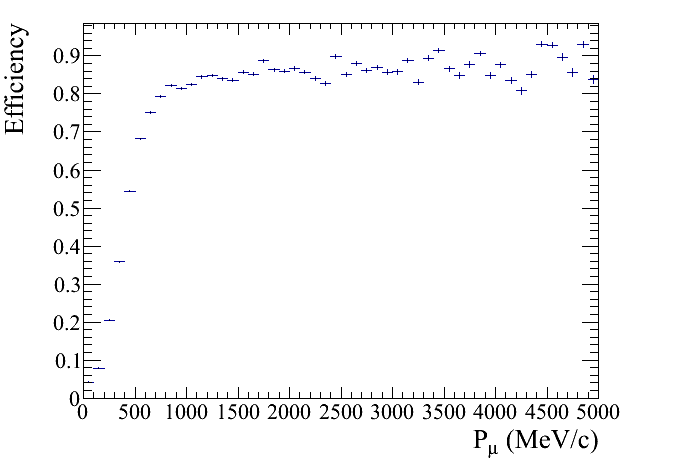
\includegraphics[width=1.0\linewidth]{figs/effmomfgd1numu}
  \caption{FGD1 $p_{\mu}$}
\end{subfigure}
\begin{subfigure}{.49\textwidth}
  \centering
  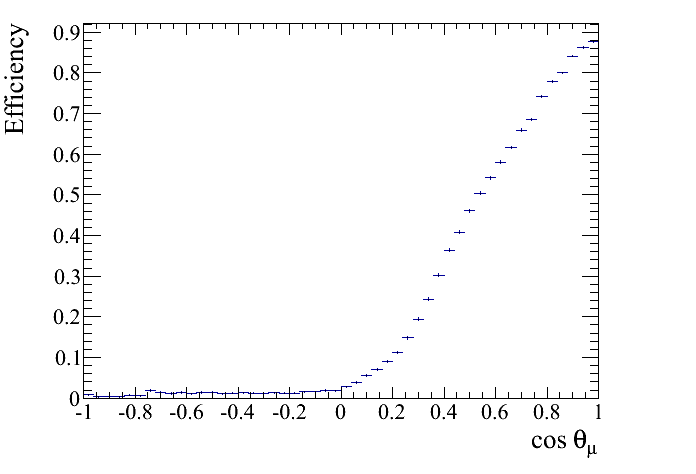
\includegraphics[width=1.0\linewidth]{figs/effcosfgd1numu}
  \caption{FGD1 cos$\theta_{\mu}$}
\end{subfigure} \\
\begin{subfigure}{.49\textwidth}
  \centering
  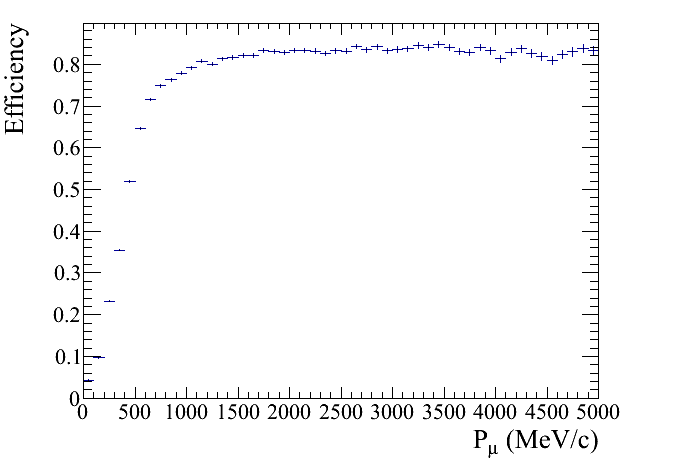
\includegraphics[width=1.0\linewidth]{figs/effmomfgd2numu}
  \caption{FGD2 $p_{\mu}$}
\end{subfigure}
\begin{subfigure}{.49\textwidth}
  \centering
  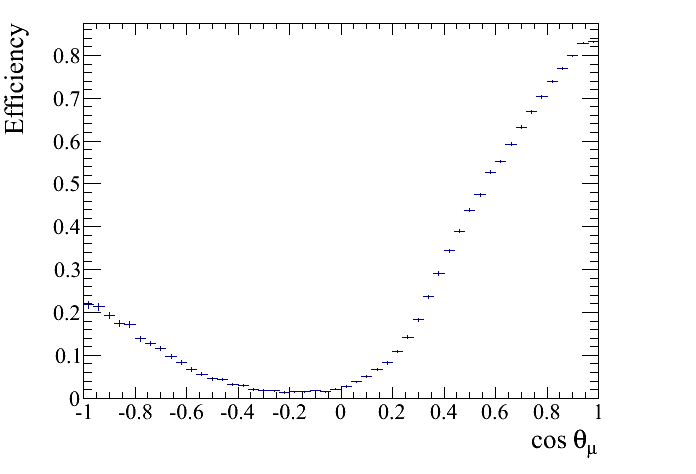
\includegraphics[width=1.0\linewidth]{figs/effcosfgd2numu}
  \caption{FGD2 cos$\theta_{\mu}$}
\end{subfigure}
\caption{Efficiency of the FGD1 and FGD2 FHC $\nu_{\mu}$ CC-inclusive samples, as a function of $p_{\mu}$ and cos$\theta_{\mu}$.}
\label{fig:numueff}
\end{figure}

This CC-inclusive selection is then divided by $\pi$ multiplicity, which depends on the identification of pions. This is done in the TPCs and FGDs:

\begin{itemize}

\item \textbf{Secondary Track:} A secondary track separate from the muon candidate must be present in the event. Events with no other track can't have a reconstructed pion, so cannot be treated as CC 1$\pi$ or Other.

\item \textbf{Bunch Matching:} The secondary track must be in the same time bunch as the muon candidate track. This cut rejects secondary tracks which are likely not from the same event.

\item \textbf{Track Start Matching:} The secondary track must originate from the fiducial volume of the same FGD as the muon candidate track. Secondary tracks starting in a different detector are likely not from the same interaction so are rejected.

\item \textbf{TPC Matching:} If the secondary and muon candidate tracks start in FGD1, the secondary track must also enter TPC 2. If the secondary and muon candidate tracks start in FGD2, the secondary track must also enter TPC 3. This cut ensures the secondary track is forward-going and long enough to be reconstructed.

\item \textbf{TPC Quality:} There must be at least 18 clusters in the TPC. This cut ensures the track is large enough to be accurately reconstructed.

\item \textbf{Pion PID:} The number of charged pions is determined by the number of secondary tracks with PID determined in the TPC corresponding to a pion. For positive tracks, the pion, positron and proton hypotheses are tested. For negative tracks, only the pion and electron hypotheses are tested. The pulls for each hypothesis are calculated and electrons are rejected by requiring:

\begin{equation}
\frac{L_{\mu}+L_{\pi}}{1-L_P} > 0.8,
\end{equation}

for tracks with $p < 500$ MeV/c. Muons and protons are then rejected by requiring:

\begin{equation}
L_{\pi} > 0.3.
\end{equation}

The number of neutral pions is determined from the presence of positrons and electrons produced in their decay.

There are two methods by which information from an FGD can be used to identify if a particle with momentum too low or angle too high to enter a TPC is a pion. However, this can only be done for charged pions as electrons and positrons are not reconstructed. 

\begin{itemize}

\item \textbf{FGD Reconstruction:} Secondary tracks in the FGD that don't start in the fiducial volume of the same FGD as the HMNT, or that aren't fully contained within the FGD, are rejected. Tracks that pass this cut and are in the same time bunch as the muon candidate are considered as pion candidates. The deposited energy in the FGD is then used to discriminate charged pions from protons.

\item \textbf{Michel Electron:} Lower momentum pions which don't produce a track in an FGD can be identified from the Michel electron produced from the muon produced in the pion decay. To be identified as the delayed signal from a Michel electron, the hit cluster must have at least 7 hits in FGD1 or 6 hits in FGD2, and be outside the beam bunch window\footnote{The muon has a 2.19 $\mu$s decay time, causing the delay in the Michel electron signal}.

\end{itemize}
\end{itemize}

The number of pions identified by the TPC PID, Michel electron tagging, and FGD PID is then used to split the CC-inclusive selection into CC 0$\pi$, CC 1$\pi$ and CC Other:

\begin{itemize}

\item \textbf{CC 0$\pi$:} Contains events with no identified charged pions, electrons or positrons using TPC PID, no Michel electrons or charged pions in either FGD, and one negative muon candidate. 

\item \textbf{CC 1$\pi$:} Contains events where the sum of the number of positive pions identified in a TPC and the number of Michel electrons is one. For events with no Michel electrons the sum of positive pions in any TPC or FGD is one. Events with a negative pion, electron, or positron reconstructed in a TPC are rejected. It is also required there is one negative muon candidate.

\item \textbf{CC Other:} Contains all events in the CC-inclusive selection that do not fall into the CC 0$\pi$ or CC 1$\pi$ sample. These are events with one negative muon candidate and either one or more reconstructed negative pions, one or more neutral pions reconstructed as electrons or positrons, or more than one positive pion reconstructed using TPC and FGD information.

\end{itemize}

\subsection{RHC $\bar{\nu_{\mu}}$}

The RHC $\bar{\nu_{\mu}}$ selections are designed to initially produce a sample of CC-inclusive interactions which occur in FGD1 or FGD2, similarly as for the FHC $\nu_{\mu}$ samples. However, events must contain one reconstructed muon track of positive charge crossing the following TPC. The selection criteria are similar as those for the FHC $\nu_{\mu}$ samples, but have extra cuts to account for the larger wrong sign background due to neutrinos having a larger cross-section on matter than anti-neutrinos:

\begin{itemize}

\item \textbf{HMT:} The background of $\nu$ events producing a $\pi^+$ misidentified as a $\mu^+$ are reduced by requiring that the highest momentum positive track (HMPT) is the highest momentum track (HMT) in the event.

\item \textbf{Upstream Background Veto:} This cut is more stringent for the RHC $\bar{\nu_{\mu}}$ samples than for FHC $\nu_{\mu}$. Events with tracks entering the fiducial volume of FGD1 from the upstream edge or coming from the P0D or magnet are rejected.

\item \textbf{Muon PID:} PID is performed using the energy deposited in the TPC and calculating the likelihood for different particle hypotheses, in the same way as for FHC $\nu_{\mu}$ samples. However, there are different requirements on the likelihoods for a positive muon candidate to be confirmed. Electrons are rejected by requiring:

\begin{equation}
\frac{L_{\mu}+L_{\pi}}{1-L_P} > 0.9,
\end{equation}

for tracks with  $p < 500$ MeV/c. Protons and pions are then rejected by requiring:

\begin{equation}
L_{\mu} > 0.1.
\end{equation}

\end{itemize}

The efficiency of the FGD1 and FGD2 RHC $\bar{\nu_{\mu}}$ CC-inclusive samples are shown in Figure \ref{fig:numueff}.  The efficiencies are higher at larger $p_{\mu}$ and cos$\theta_{\mu}$. 

\begin{figure}[t]
\centering
\begin{subfigure}{.49\textwidth}
  \centering
  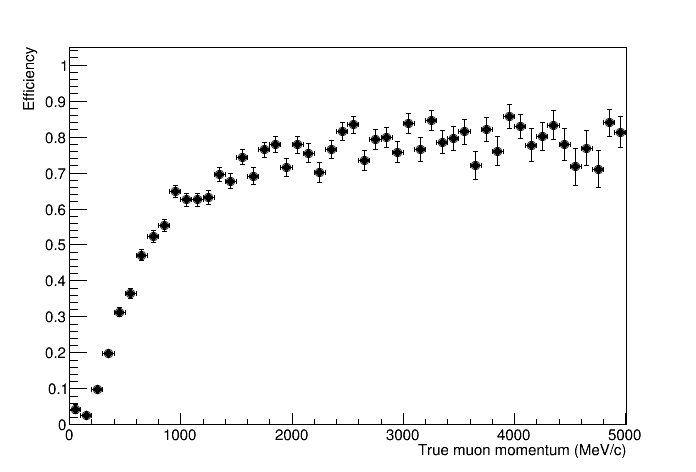
\includegraphics[width=1.0\linewidth]{figs/effmomfgd1numubar}
  \caption{FGD1 $p_{\mu}$}
\end{subfigure}
\begin{subfigure}{.49\textwidth}
  \centering
  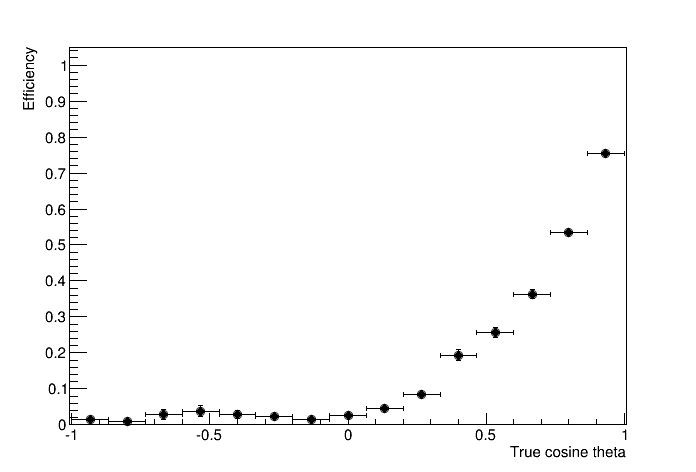
\includegraphics[width=1.0\linewidth]{figs/effcosfgd1numubar}
  \caption{FGD1 cos$\theta_{\mu}$}
\end{subfigure} \\
\begin{subfigure}{.49\textwidth}
  \centering
  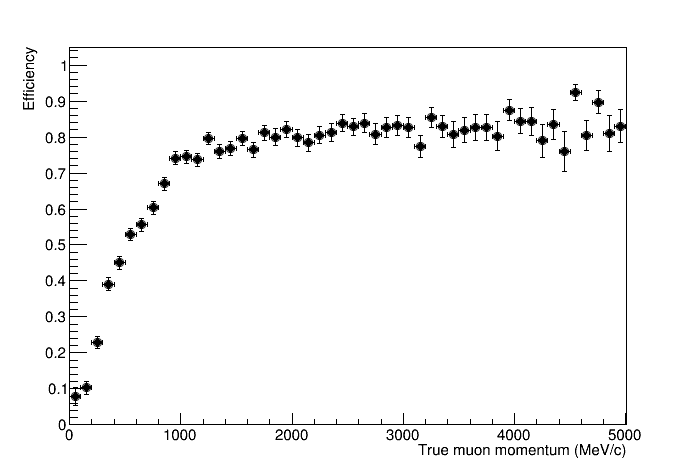
\includegraphics[width=1.0\linewidth]{figs/effmomfgd2numubar}
  \caption{FGD2 $p_{\mu}$}
\end{subfigure}
\begin{subfigure}{.49\textwidth}
  \centering
  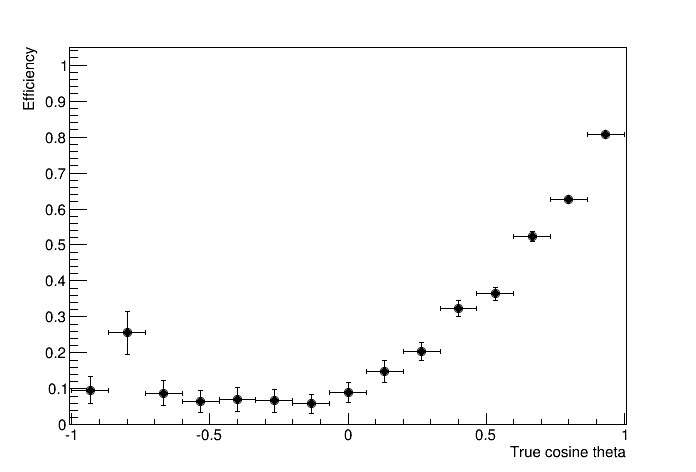
\includegraphics[width=1.0\linewidth]{figs/effcosfgd2numubar}
  \caption{FGD2 cos$\theta_{\mu}$}
\end{subfigure}
\caption{Efficiency of the FGD1 and FGD2 RHC $\bar{\nu_{\mu}}$ CC inclusive samples, as a function of $p_{\mu}$ and cos$\theta_{\mu}$.}
\label{fig:numubareff}
\end{figure}

The pion identification is performed in the same way as for FHC $\nu_{\mu}$, and the CC-inclusive sample is again split into CC 0$\pi$, CC 1$\pi$ and CC Other.

\subsection{RHC $\nu_{\mu}$}

In RHC mode, there are still a significant number of $\nu$ events due to the larger $\nu$ cross-section, and so a selection of these events is made. The same cuts as for the FHC $\nu_{\mu}$ and RHC $\bar{\nu_{\mu}}$ are applied, but with the following exceptions:

\begin{itemize}

\item \textbf{HMT:} It is required that the HMNT  in the event is the HMT.

\item \textbf{Upstream Background Veto:} As for the RHC $\bar{\nu_{\mu}}$ samples, events with tracks entering the fiducial volume of FGD1 from the upstream edge or coming from the P0D or magnet are rejected.

\item \textbf{Muon PID:} PID is performed in the same way as for the previous samples, using the energy deposited in the TPC and calculating the likelihood for different particle hypotheses. However, there are different requirements on the likelihoods for a negative muon candidate to be confirmed. Electrons are rejected by requiring:

\begin{equation}
\frac{L_{\mu}+L_{\pi}}{1-L_P} > 0.7,
\end{equation}

for tracks with  $p <$ 500 MeV/c. Protons and pions are then rejected by requiring:

\begin{equation}
L_{\mu} > 0.1.
\end{equation}

\end{itemize}

The efficiency of the FGD1 and FGD2 RHC $\nu_{\mu}$ CC-inclusive samples are shown in Figure \ref{fig:nuinnubareff}. The efficiencies are higher at larger $p_{\mu}$ and cos$\theta_{\mu}$.

\begin{figure}
\centering
\begin{subfigure}{.49\textwidth}
  \centering
  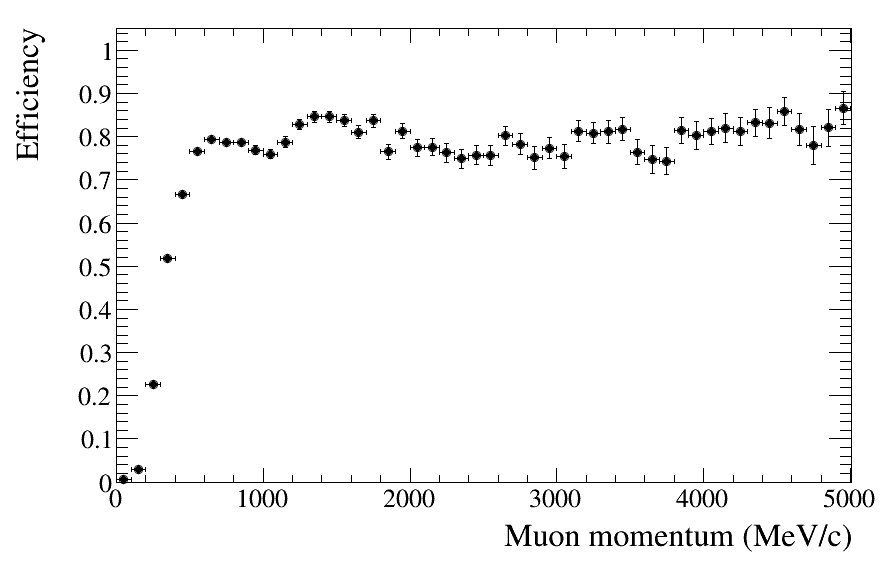
\includegraphics[width=1.0\linewidth]{figs/effmomfgd1nuinnubar}
  \caption{FGD1 $p_{\mu}$}
\end{subfigure}
\begin{subfigure}{.49\textwidth}
  \centering
  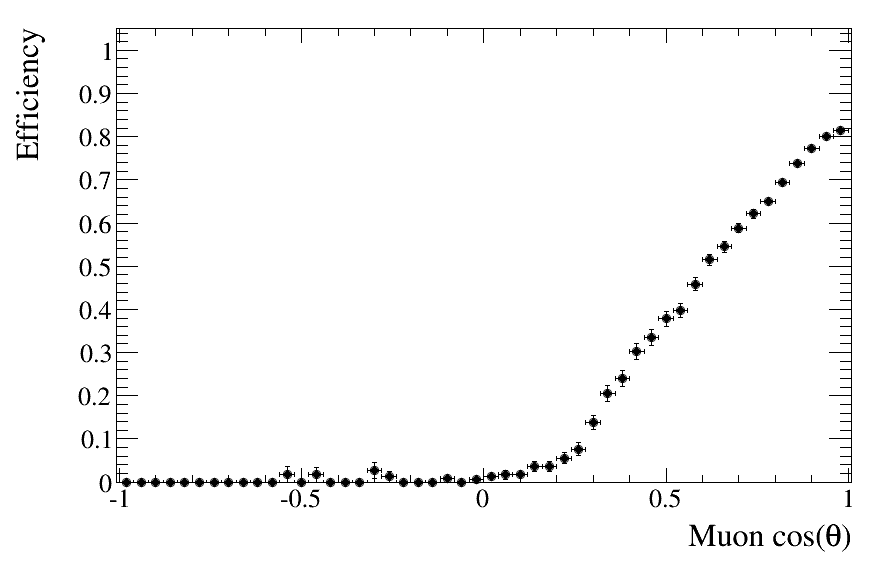
\includegraphics[width=1.0\linewidth]{figs/effcosfgd1nuinnubar}
  \caption{FGD1 cos$\theta_{\mu}$}
\end{subfigure} \\
\begin{subfigure}{.49\textwidth}
  \centering
  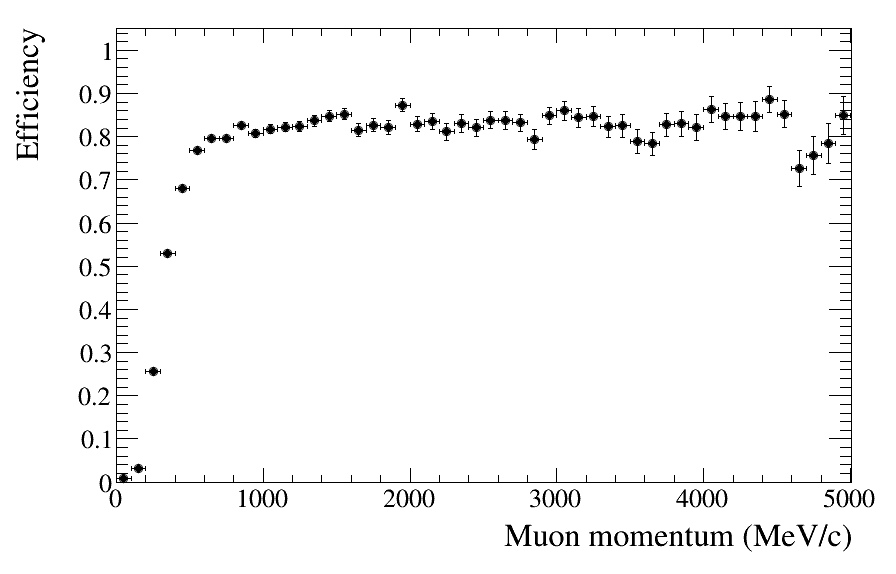
\includegraphics[width=1.0\linewidth]{figs/effmomfgd2nuinnubar}
  \caption{FGD2 $p_{\mu}$}
\end{subfigure}
\begin{subfigure}{.49\textwidth}
  \centering
  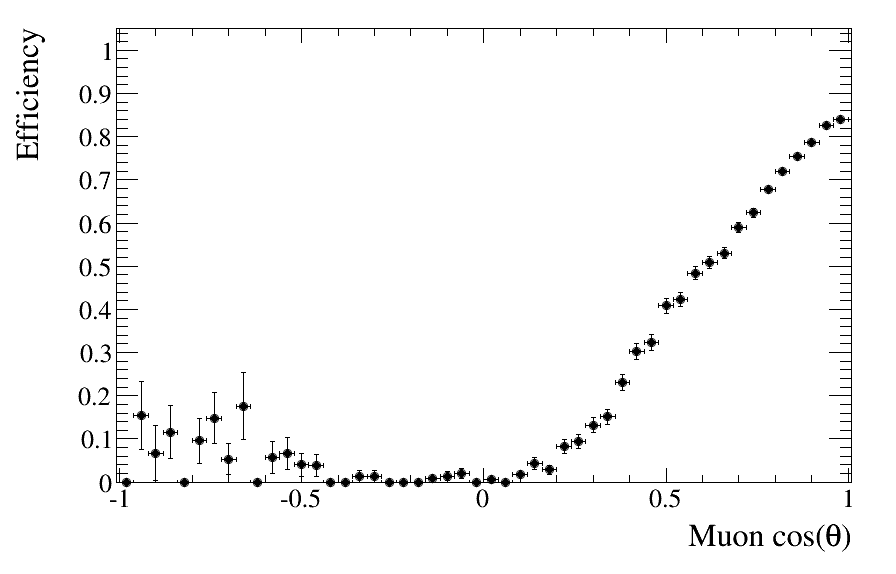
\includegraphics[width=1.0\linewidth]{figs/effcosfgd2nuinnubar}
  \caption{FGD2 cos$\theta_{\mu}$}
\end{subfigure}
\caption{Efficiency of the FGD1 and FGD2 RHC $\nu_{\mu}$ CC inclusive samples, as a function of $p_{\mu}$ and cos$\theta_{\mu}$.}
\label{fig:nuinnubareff}
\end{figure}

\subsection{Updating to RHC Multi $\pi$ Samples}

In previous analyses, the RHC CC-inclusive samples were divided by track, rather than $\pi$ multiplicity, into CC 1Track and CC NTracks. Before the 2020 analysis, there were much fewer RHC data events than FHC, and so the RHC samples could not be divided into so many sub-samples. In moving to RHC multi-$\pi$, the FHC selection criteria was unchanged, and the RHC selections only changed in the likelihood cuts for rejecting the proton and pion hypotheses in muon identification:

\begin{equation}
0.1 < L_{\mu} < 0.7.
\end{equation}

The upper bound was designed to reject low momentum wrong sign muons in RHC events, which could be misreconstructed as positive tracks.

The previous RHC sample splitting proceeded by selecting events with one positive muon and no charged or neutral pions in the CC 1Track sample, and selecting all other CC-inclusive events in the CC NTracks sample. Validations of the updating of the fitting framework to accommodate the RHC multi-$\pi$ samples are presented in Appendix \ref{appendix:rhcmpi}.

\section{Binning}\label{sec:binning}

ND280 events are binned in the reconstructed momentum and angle of the outgoing lepton. The choice of binning is a trade-off of having coarse enough bins to have enough events in each to reduce the statistical error, while being fine enough to have good resolution in the peak regions. In general, the aim is to have $>$20 raw MC events in every bin, which is approximately equivalent to having $\sim$1-2 data events. Achieving this using uniform rectangular binning can result in bins outside the region of interest containing the largest amount of events, and contributing the most to the sample log-likelihood. Figure \ref{fig:th2dbin} shows this effect in the FHC CC 0$\pi$ and CC 1$\pi$ sample binnings used for the 2017 oscillation analysis. These plots only show up to 5000 MeV to show the peak regions more clearly. The full binning used here was the same for FGD1 and FGD2, and is as follows:

\begin{itemize}

\item \textbf{FHC $\nu_{\mu}$ CC 0$\pi$:}\\
\textbf{\textit{p} (MeV/c):} 0, 200, 300, 400, 450, 500, 550, 600, 650, 700, 750, 800, 850, 900, 950, 1000, 1050, 1100, 1200, 1300, 1400, 1500, 1600, 1700, 1800, 2000, 2500, 3000, 5000, 30000.\\
\textbf{cos $\theta$:} -1, 0.5, 0.6, 0.7, 0.76, 0.78, 0.8, 0.83, 0.85, 0.88, 0.89, 0.9, 0.91, 0.92, 0.925, 0.93, 0.935, 0.94, 0.945, 0.95, 0.955, 0.96, 0.965, 0.97, 0.975, 0.98, 0.985, 0.99, 0.995, 1.

\item \textbf{FHC $\nu_{\mu}$ CC 1$\pi$:}\\
\textbf{\textit{p} (MeV/c):} 0, 300, 350, 400, 500, 600, 650, 700, 750, 800, 900, 1000, 1100, 1200, 1500, 2000, 3000, 5000, 30000.\\
\textbf{cos $\theta$:} -1, 0.6, 0.7, 0.8, 0.85, 0.88, 0.9, 0.92, 0.93, 0.94, 0.95, 0.96, 0.97, 0.98, 0.99, 0.995, 1.

\item \textbf{FHC $\nu_{\mu}$ CC Other:}\\
\textbf{\textit{p} (MeV/c):} 0, 300, 400, 500, 600, 650, 700, 750, 800, 900, 1000, 1100, 1250, 1500, 1750, 2000, 3000, 5000, 30000.\\
\textbf{cos $\theta$:} -1, 0.6, 0.7, 0.76, 0.8, 0.85, 0.88, 0.89, 0.9, 0.91, 0.92, 0.93, 0.94, 0.95, 0.96, 0.97, 0.98, 0.99, 0.995, 1.

\item \textbf{RHC $\bar{\nu_{\mu}}$ CC 0$\pi$:}\\
\textbf{\textit{p} (MeV/c):} 0, 300, 400, 500, 550, 600, 650, 700, 750, 800, 900, 1000, 1100, 1200, 1500, 2000, 4000, 30000.\\
\textbf{cos $\theta$:} -1, 0.6, 0.7, 0.8, 0.85, 0.9, 0.92, 0.93, 0.94, 0.95, 0.96, 0.965, 0.97, 0.975, 0.98, 0.985, 0.99, 0.995, 1.

\item \textbf{RHC $\bar{\nu_{\mu}}$ CC 1$\pi$:}\\
\textbf{\textit{p} (MeV/c):} 0, 500, 700, 900, 1300, 2500, 30000.\\
\textbf{cos $\theta$:}  -1, 0.7, 0.8, 0.9, 0.94, 0.96, 0.98, 0.99, 1.

\item \textbf{RHC $\bar{\nu_{\mu}}$ CC Other:}
\textbf{\textit{p} (MeV/c):} 0, 600, 800, 1000, 1250, 1500, 2000, 4000, 30000.\\
\textbf{cos $\theta$:} -1, 0.7, 0.8, 0.85, 0.9, 0.93, 0.95, 0.97, 0.98, 0.99, 1.

\item \textbf{RHC $\nu_{\mu}$ CC 0$\pi$:}\\
\textbf{\textit{p} (MeV/c):} 0, 300, 500, 700, 800, 900, 1250, 1500, 2000, 4000, 30000.\\
\textbf{cos $\theta$:} -1, 0.7, 0.8, 0.85, 0.88, 0.9, 0.92, 0.94, 0.96, 0.97, 0.98, 0.99, 1.

\item \textbf{RHC $\nu_{\mu}$ CC 1$\pi$:}\\
\textbf{\textit{p} (MeV/c):} 0, 600, 800, 1500, 30000.\\
\textbf{cos $\theta$:} -1, 0.7, 0.8, 0.86, 0.9, 0.94, 0.96, 0.97, 0.98, 0.99, 1.

\item \textbf{RHC $\nu_{\mu}$ CC Other:}\\
\textbf{\textit{p} (MeV/c):} 0, 600, 1000, 1250, 2000, 4000, 30000.\\
\textbf{cos $\theta$:} -1, 0.7, 0.8, 0.86, 0.9, 0.93, 0.95, 0.97, 0.99, 1.

\end{itemize}

\begin{figure}
\centering
\begin{subfigure}{.49\textwidth}
  \centering
  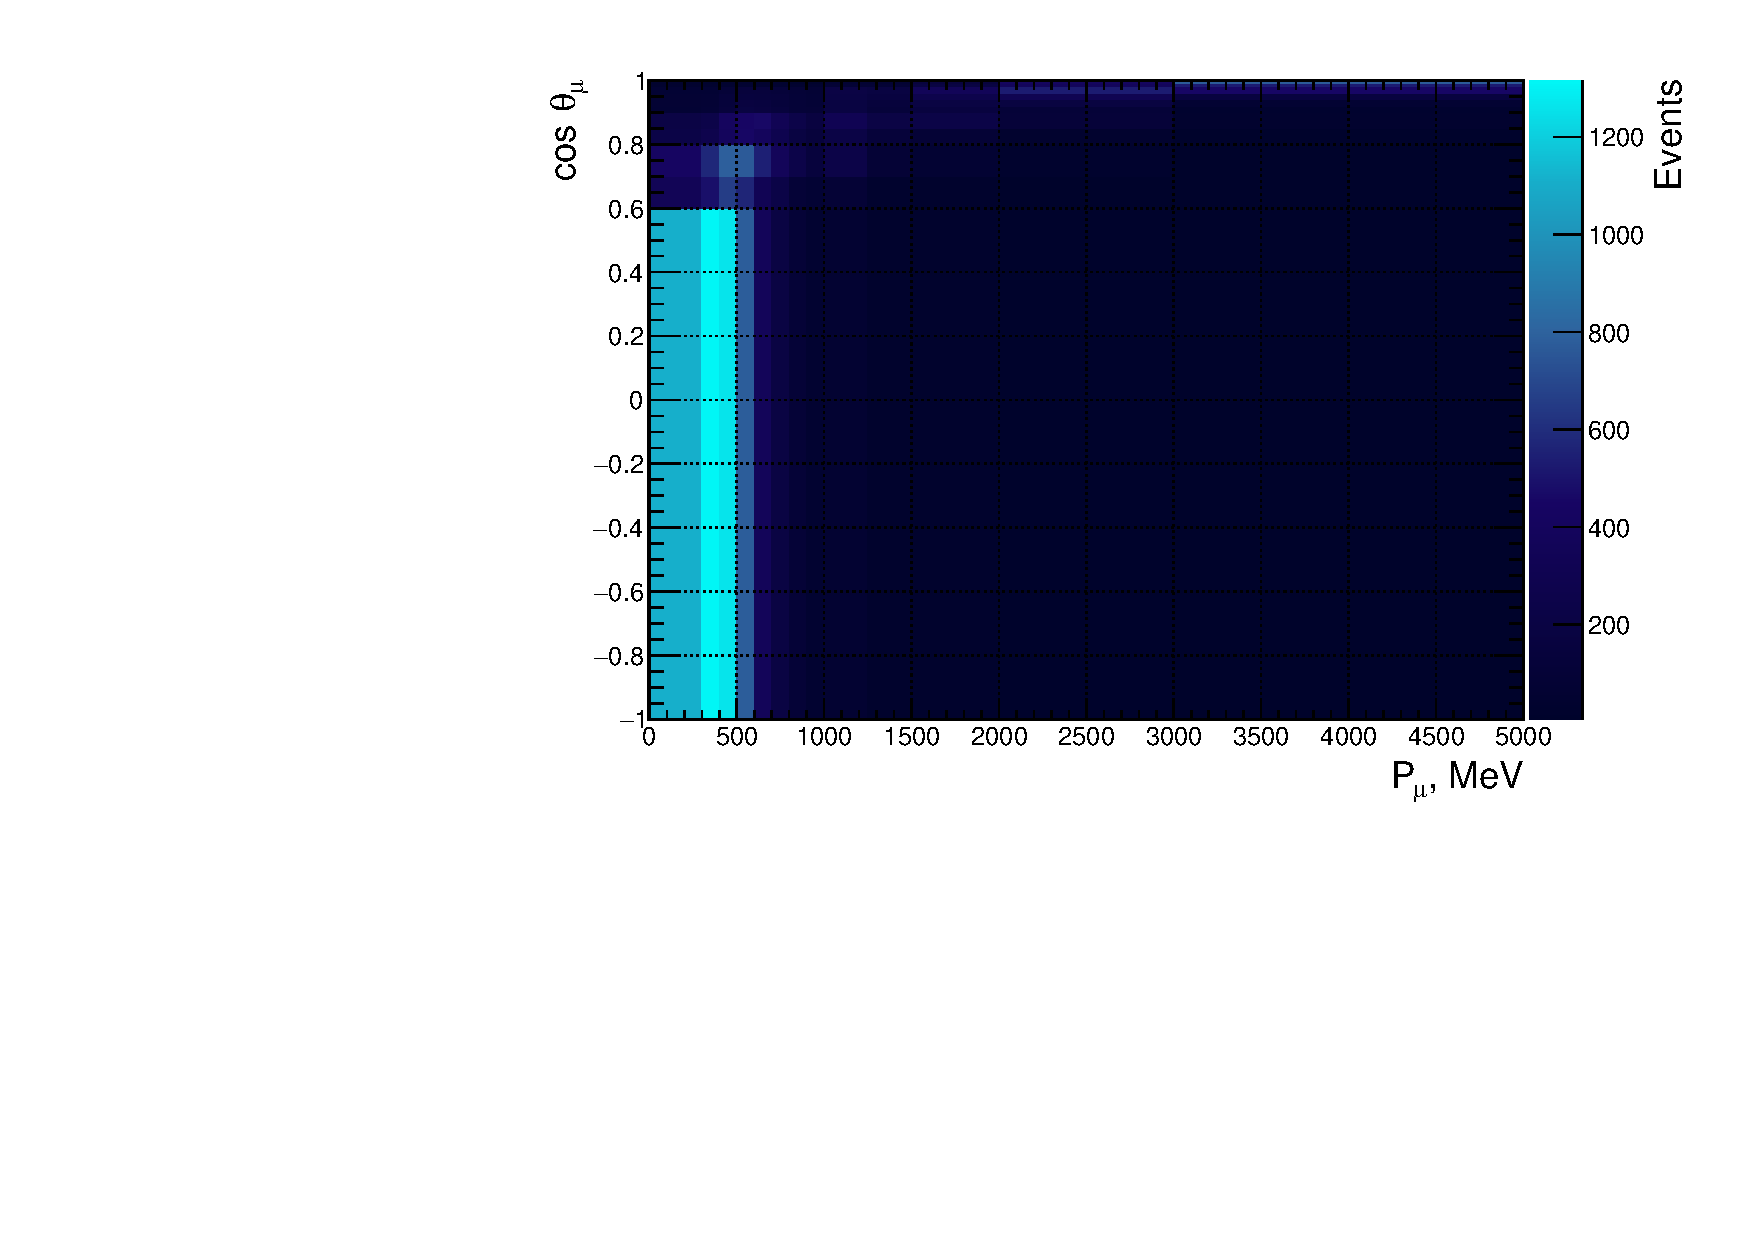
\includegraphics[width=0.95\linewidth]{figs/TH2D_MC_FGD1_numuCC_0pi}
  \caption{FGD1 FHC $\nu_{\mu}$ 0$\pi$}
  \label{fig:th2dFGD1_numuCC_0pi}
\end{subfigure}
\begin{subfigure}{.49\textwidth}
  \centering
  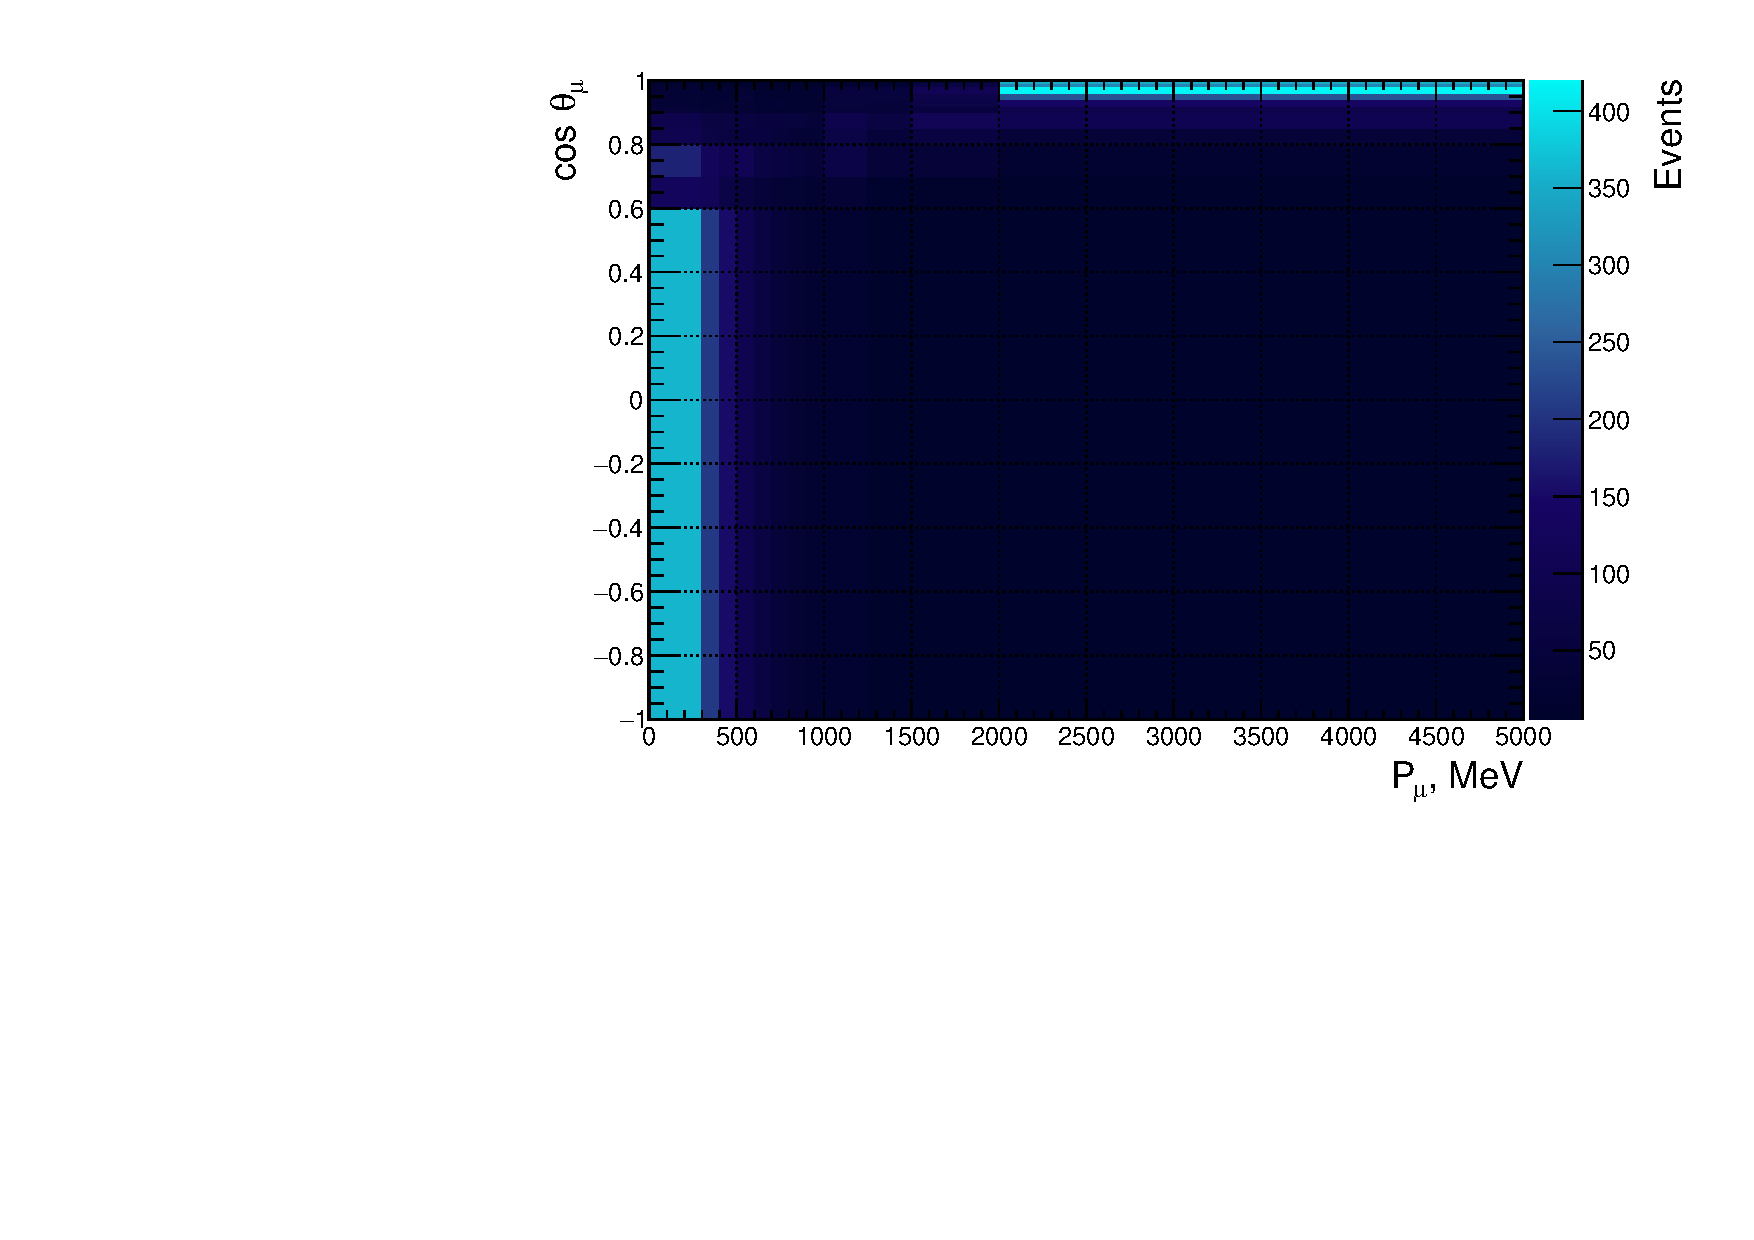
\includegraphics[width=0.95\linewidth]{figs/TH2D_MC_FGD1_numuCC_1pi}
  \caption{FGD1 FHC $\nu_{\mu}$ 1$\pi$}
  \label{fig:th2dFGD1_numuCC_1pi}
\end{subfigure}
\caption{Uniform rectangular binning of the FGD1 CC 0$\pi$ and FGD1 CC 1$\pi$ MC samples for T2K runs 2-8.}
\label{fig:th2dbin}
\end{figure}

For example, in the FGD1 CC 0$\pi$ sample, the bins at low angle, ($<0.6$), and low momentum, ($\sim$500 MeV), the bins span a large angle range (-1.0 - 0.6). Having such large bins causes them to contain a large amount of events. However, if they were divided to only span a smaller range of angles, the bins at the same angle but higher momentum would also be divided. As these regions are much more sparsely populated, splitting them further would result in there being insufficient number of events in those bins. The same is true for the high angle bins at higher momentum. These bins cover a large momentum range and are well populated; there are a relatively large amount of events with high momentum forward-going muons. Splitting these bins though would mean the backward-going bins at the same high momentum would not be large enough and so would be too sparsely populated. This effect becomes more significant with the addition of more data.

\subsection{Non-Uniform Rectangular Binning Studies}\label{sec:nonrecbinning}
\enlargethispage{\baselineskip}
For the 2020 analysis, the MaCh3 near detector framework was updated to be able to use non-uniform rectangular binning\footnote{Mechanically, this meant using ROOT\cite{root} TH2Poly objects instead of TH2Ds.}. This means the bins can now be any arbitrary shape, including the original uniform rectangular binning which can still be used for validations of the changes to the fitting framework, and cross-group checks with the other near detector fitter which did not move to non-uniform rectangular binning.

The following algorithm was used to define a non-uniform but still rectangular binning for each sample, without having to have the same binning for FGD1 and FGD2:

\begin{itemize}

\item The bin edges on the cos$\theta$ axis are hard coded and constant, guided by the previous binning, keeping the bins rectangular. The reasons for this are discussed later in this section.

\item For each cos$\theta$ row, scroll across from 30 GeV down 0 GeV in 100 MeV steps.

\item Once 50 unscaled MC events are reached, start a new bin.

\item If the last bin in a row (the lowest momentum bin) has $<$20 unscaled MC events, merge with the previous bin. Scroll through this merged bin in 5 MeV steps and split once half the events in the bin are reached.

\end{itemize}

The algorithm was tuned using data and MC from runs 2-6. The aim of this process was to produce as uniform a distribution of events across the bins as possible. This was not always possible, as regions of high density would require bins so small that they go below the resolution of the detector. The hard coded cos$\theta$ bin edges and momentum step sizes of 100 MeV were driven by this minimum bin size limit. The resolutions are calculated by plotting the reconstructed vs true kinematic variables, as shown in Figure \ref{fig:res2d}, and taking the RMS at different slices of the 2D Gaussian. These RMSs, shown in Figures \ref{fig:res1d}, give a gauge of the detector resolution, and so the minimum bin width for each variable in different regions.

For momentum, the RMS is fairly constant at approximately 100 MeV, for a momentum $>$1000 MeV. It then reduces linearly between 1000 and 400 MeV, before levelling off at approximately 60 MeV below 300 MeV. Similarly, for the angle, the RMS is constant at approximately 0.08 below 0.96. It then reduces linearly up to a cos$\theta$ of 1.0. However, given there would be a large uncertainty on the gradient for each variable's RMS, rather than varying the minimum bin size to trace out the change in RMS as closely as possible, it was safer to have a constant minimum size for all regions. This was chosen to be 0.01 cos$\theta$ in angle, and 100 MeV in momentum to be sure they are above the resolution in all regions. Furthermore, as the cos$\theta$ systematics are better controlled than for $p_{\mu}$, and for aiding the simplicity of optimising the binning algorithm, the bins were kept constant in cos$\theta$. Although these bins are conservatively large in regions with the most data, studies in reducing the bin sizes showed diminishing returns in improvements to sensitivity.

\begin{figure}[t]
\centering
\begin{subfigure}{.5\textwidth}
  \centering
  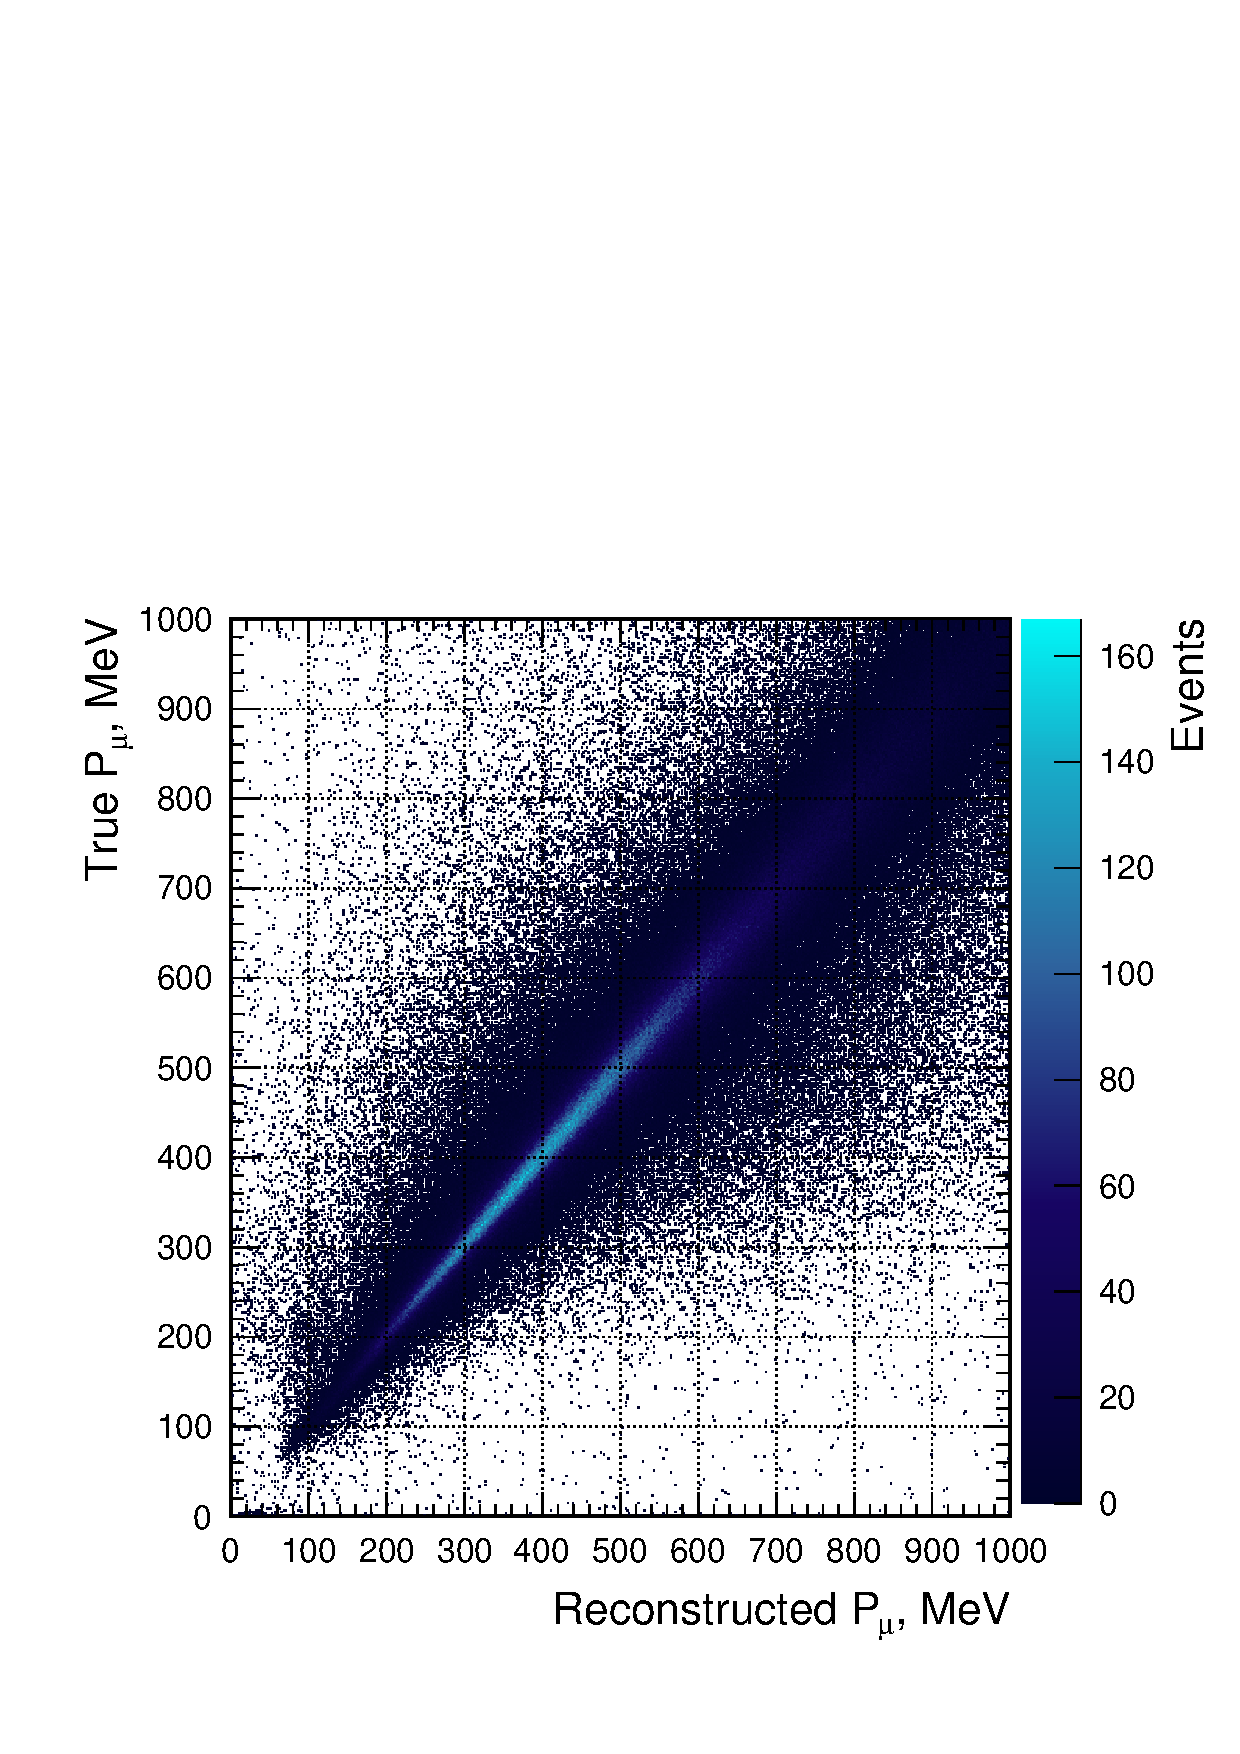
\includegraphics[width=0.95\linewidth]{figs/momres2d}
  \caption{Final state lepton momentum.}
  \label{fig:momres2d}
\end{subfigure}%
\begin{subfigure}{.5\textwidth}
  \centering
  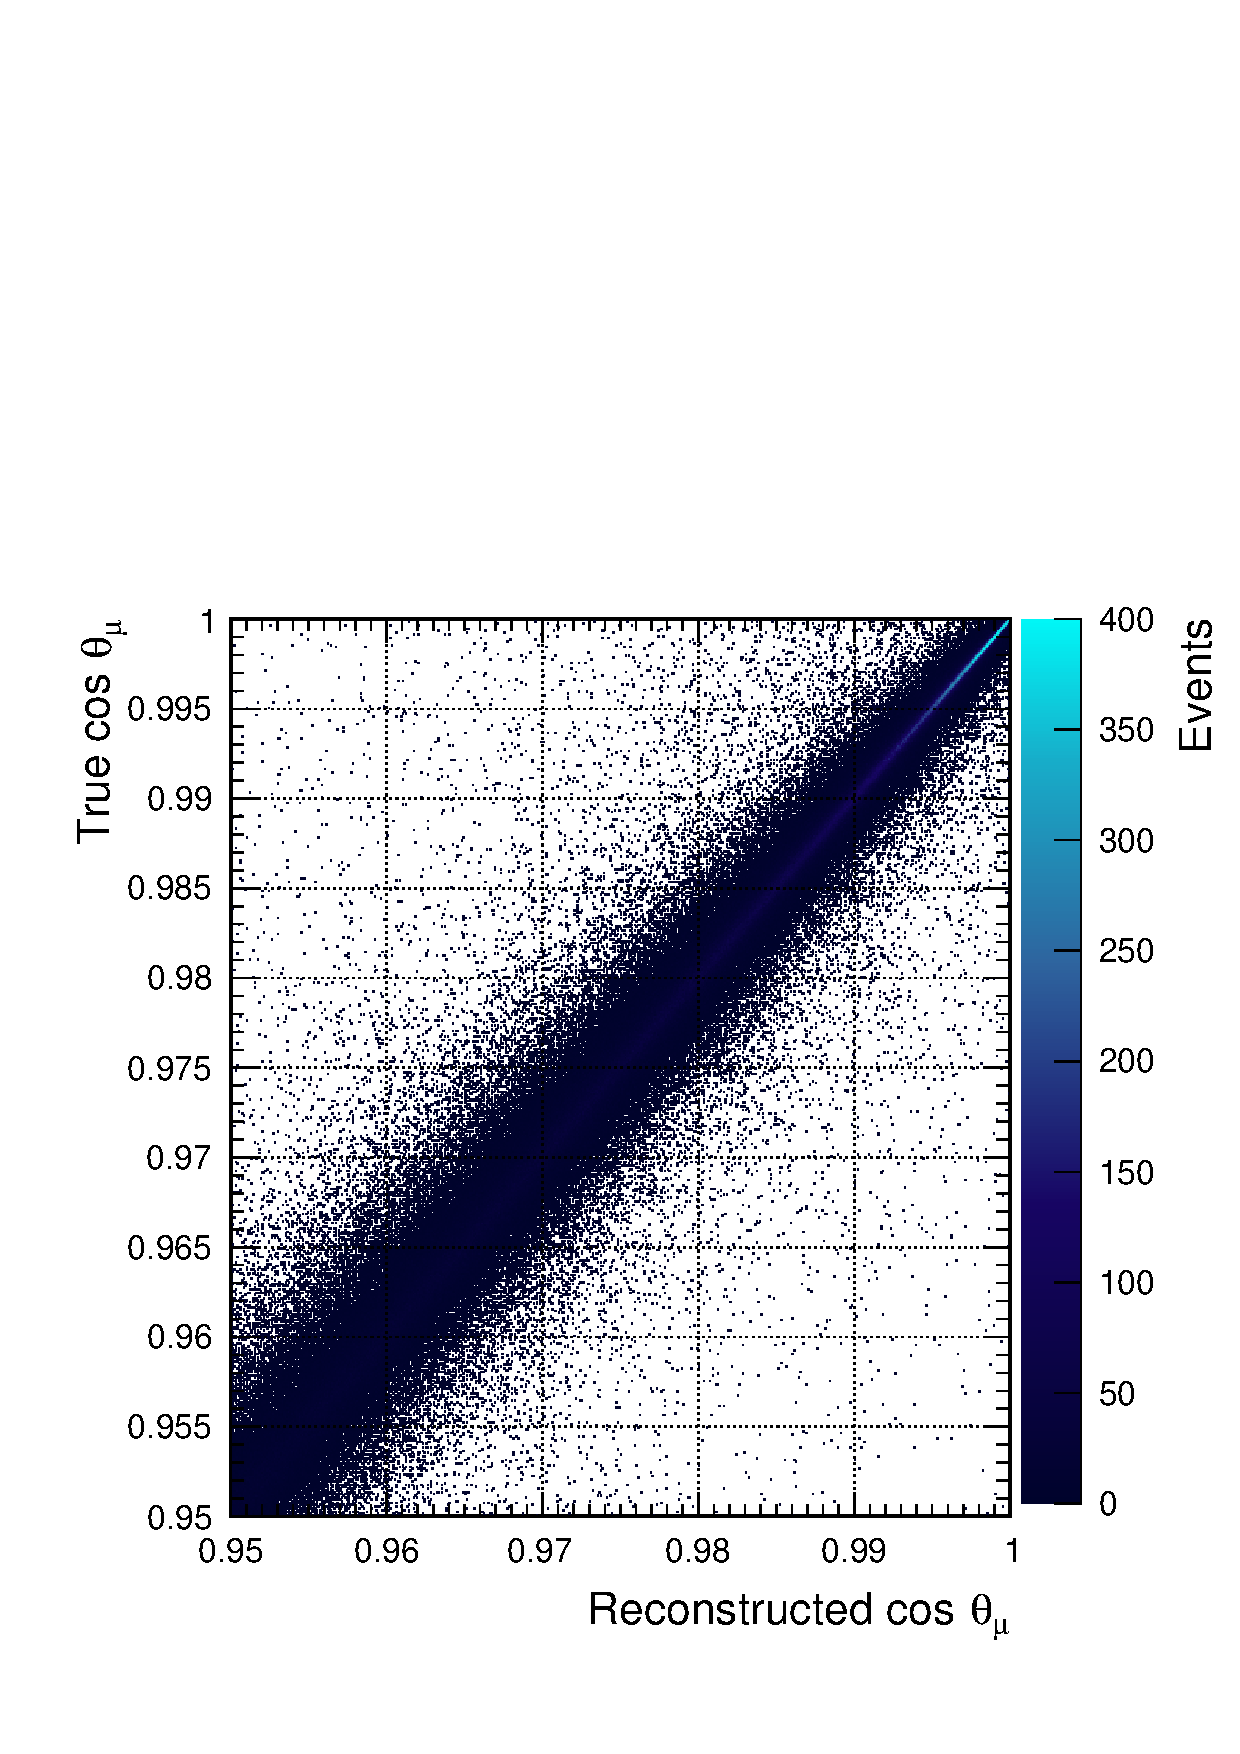
\includegraphics[width=0.95\linewidth]{figs/angres2d}
  \caption{Final state lepton angle.}
  \label{fig:angres2d}
\end{subfigure}
\caption{True vs reconstructed lepton kinematic variables of CC-inclusive MC events from T2K runs 2-8.}
\label{fig:res2d}
\end{figure}

\begin{figure}[t]
\centering
\begin{subfigure}{.5\textwidth}
  \centering
  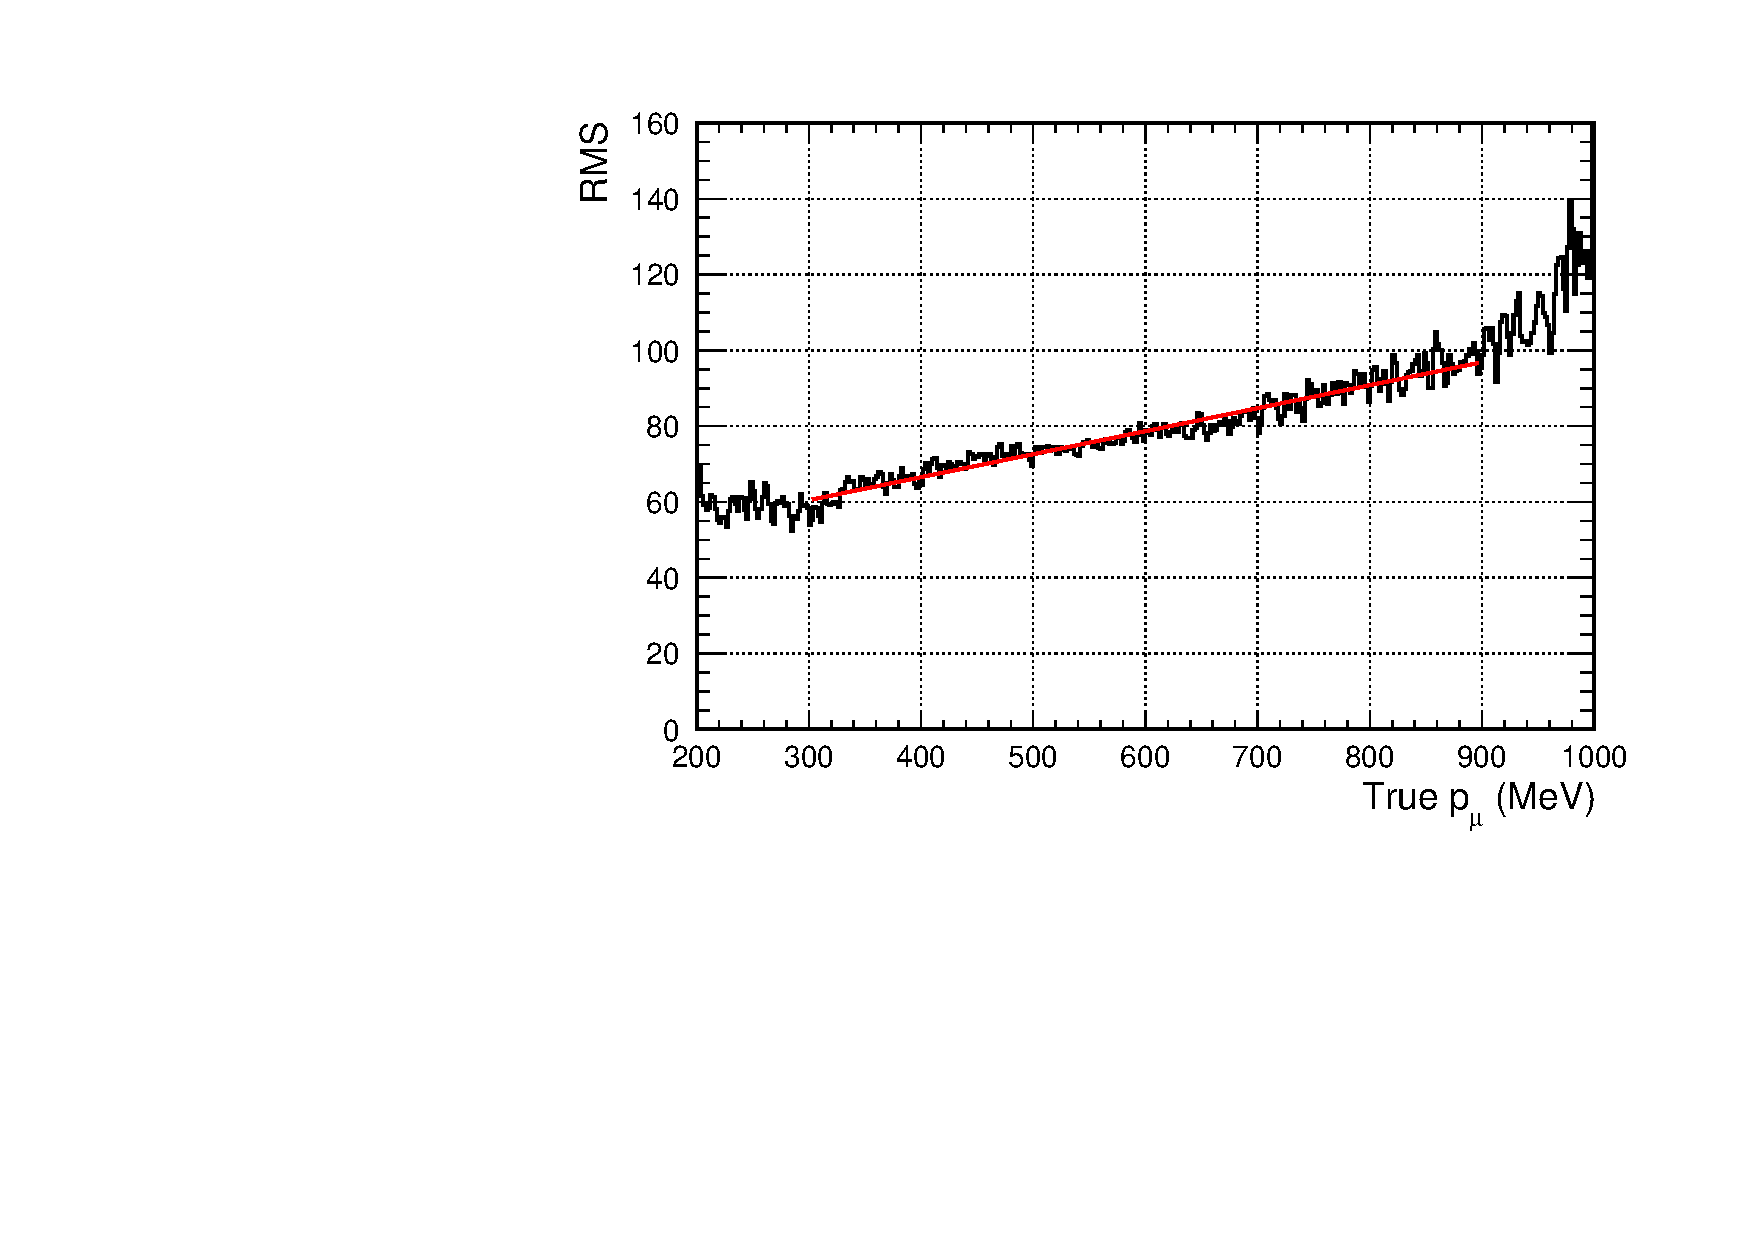
\includegraphics[width=0.95\linewidth]{figs/momres1d}
  \caption{Final state lepton momentum.}
  \label{fig:momres1d}
\end{subfigure}%
\begin{subfigure}{.5\textwidth}
  \centering
  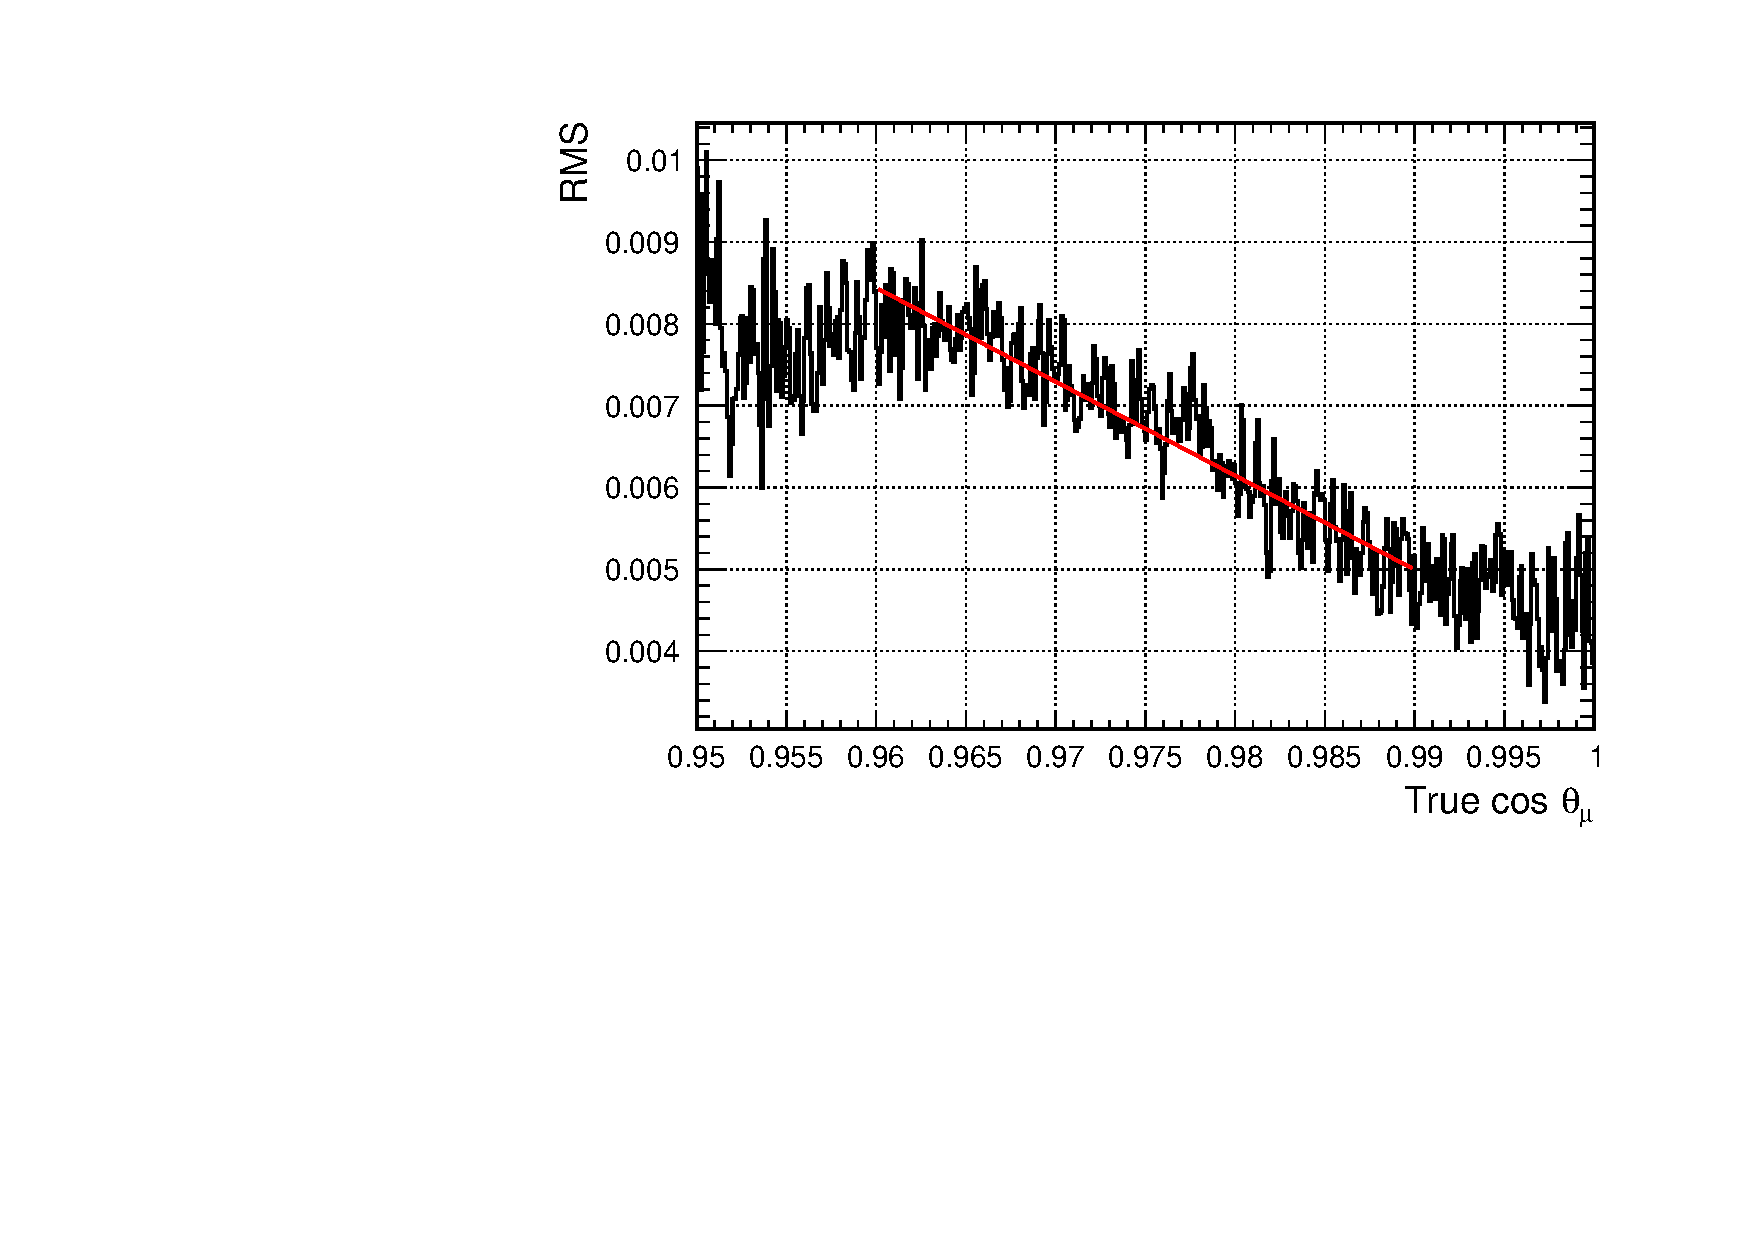
\includegraphics[width=0.95\linewidth]{figs/angres1d}
  \caption{Final state lepton angle.}
  \label{fig:angres1d}
\end{subfigure}
\caption{The RMS of the true vs reconstructed lepton kinematic variables for CC-inclusive MC events from T2K runs 2-8, at different values of the true variables.}
\label{fig:res1d}
\end{figure}

The distribution of events binned by the scheme produced using the algorithm for the FGD1 CC 0$\pi$ and CC 1$\pi$ samples are shown in Figure \ref{fig:th2polybin}. Full templates of the binning for each sample are shown in Appendix \ref{app:bintemplates}. Particularly for the FHC $\nu_{\mu}$ and RHC $\bar{\nu_{\mu}}$ CC 0$\pi$ samples, the bins containing the largest amount of events are in the peak regions at high angle and $\sim$500 MeV. However, what is of more importance is the significant reduction in ranges of the $z$ axis scales compared to the uniform binning. For example, the non-uniform binning for the RHC $\bar{\nu_{\mu}}$ CC 0$\pi$ samples may not look like the most aesthetic representation of distributions, but the bin with the most events contains less than double the amount of the bin with the least. For the uniform binning, the bin with the most events contains $\sim$250 times more than the amount in the bin with the least events. Reducing this range prevents bins outside the peak contributing more to the LLH than the region of interest.

\begin{figure}
\centering
\begin{subfigure}{.49\textwidth}
  \centering
  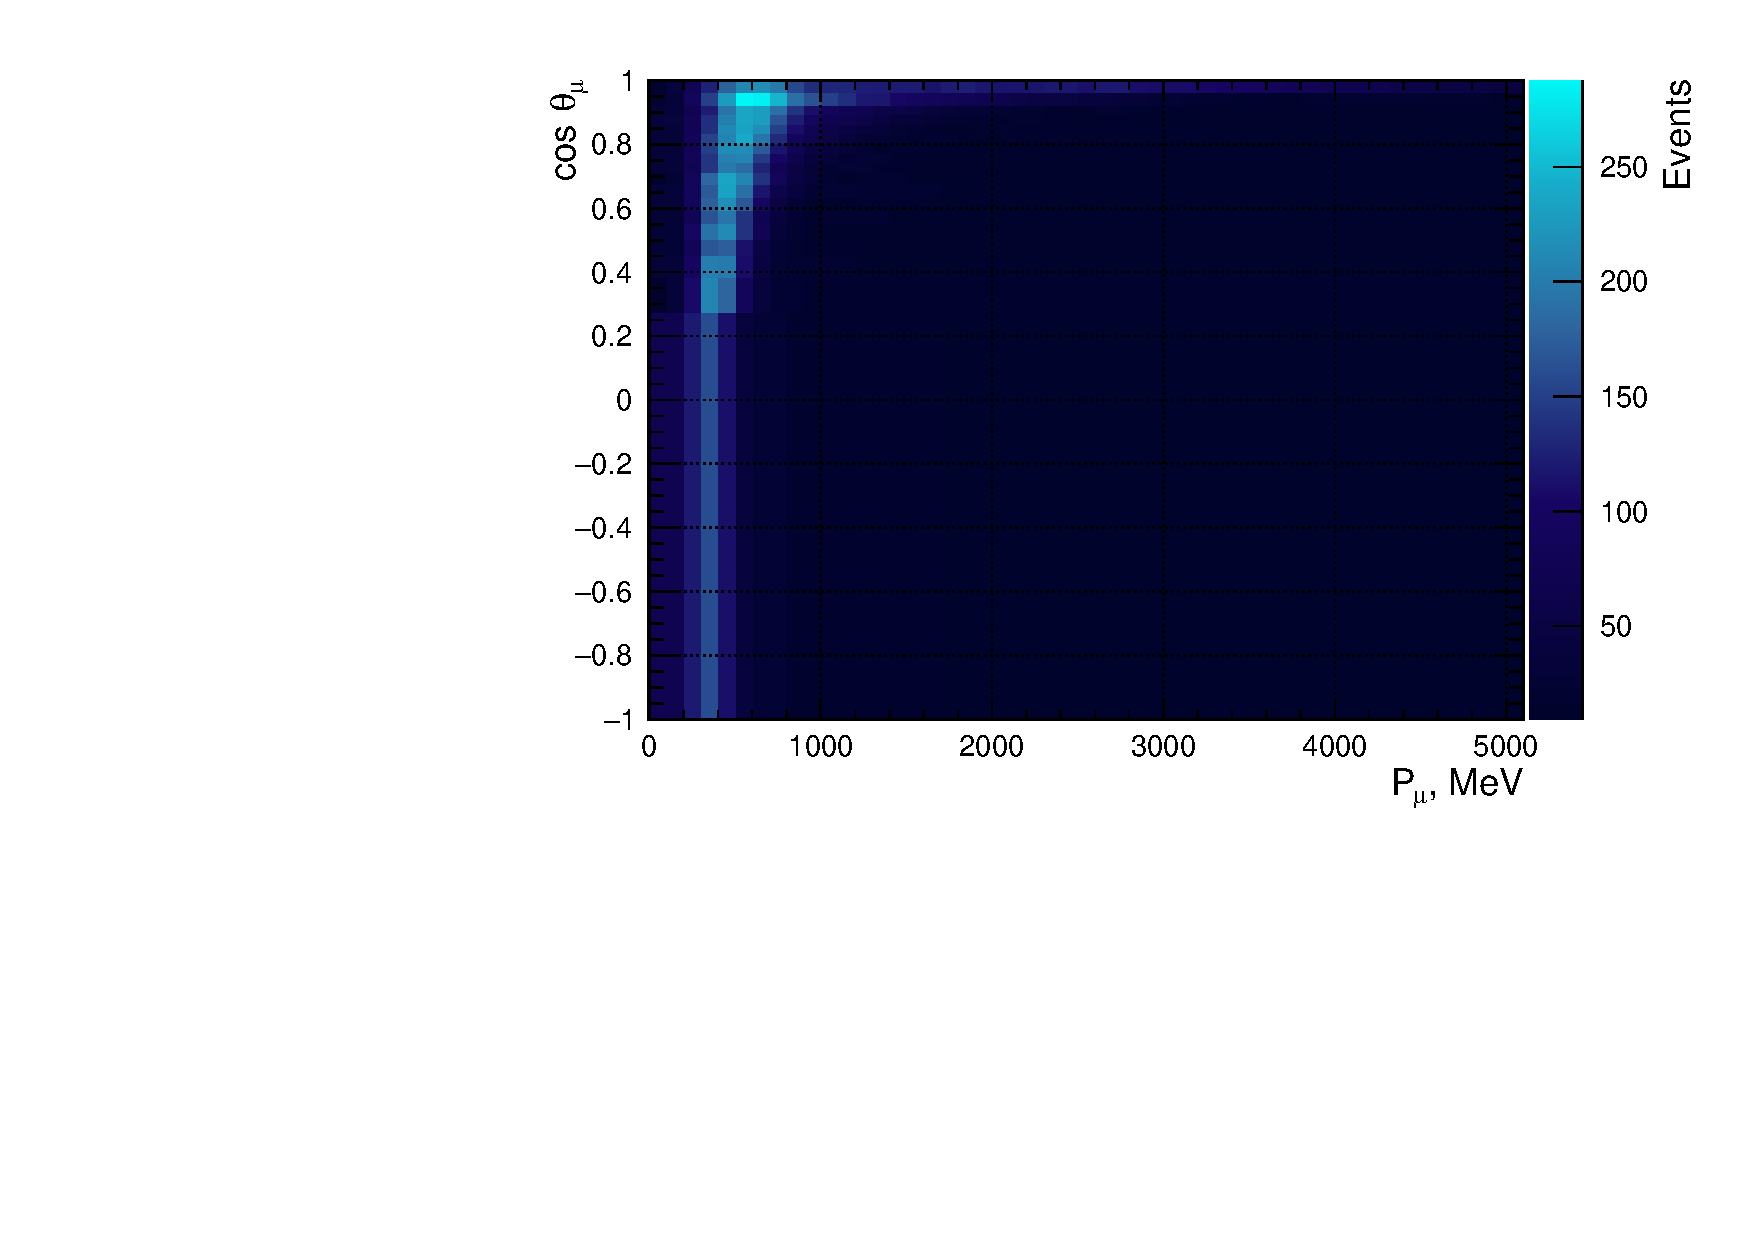
\includegraphics[width=0.95\linewidth]{figs/TH2Poly_MC_FGD1_numuCC_0pi}
  \caption{FGD1 FHC $\nu_{\mu}$ 0$\pi$}
  \label{fig:th2polyFGD1_numuCC_0pi}
\end{subfigure}
\begin{subfigure}{.49\textwidth}
  \centering
  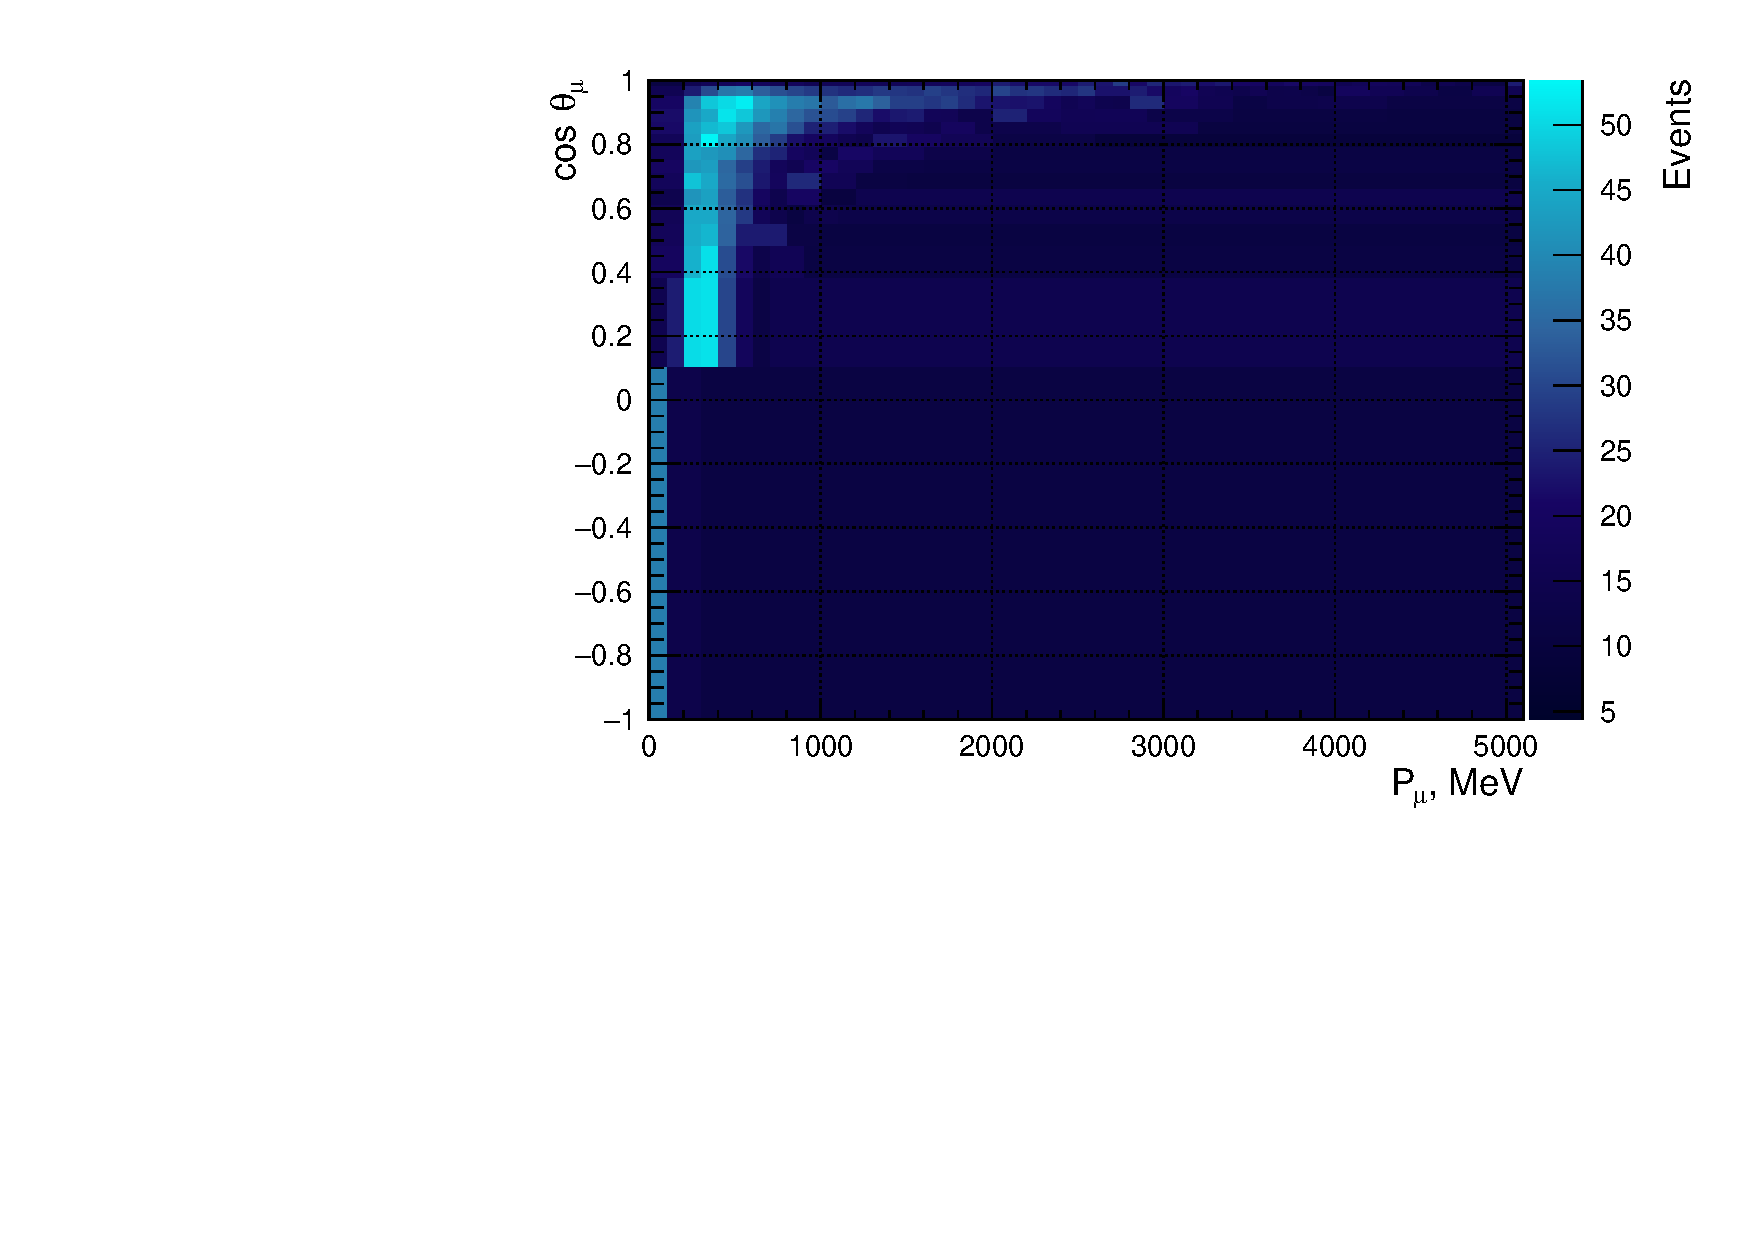
\includegraphics[width=0.95\linewidth]{figs/TH2Poly_MC_FGD1_numuCC_1pi}
  \caption{FGD1 FHC $\nu_{\mu}$ 1$\pi$}
  \label{fig:th2polyFGD1_numuCC_1pi}
\end{subfigure}
\caption{Non-uniform rectangular binning of the FGD1 CC 0$\pi$ and FGD1 CC 1$\pi$ MC samples for T2K runs 2-8.}
\label{fig:th2polybin}
\end{figure}

Using non-uniform binning significantly improves the sensitivity of the fit to changes in parameter values. This is evident in the log-likelihood scans shown in Figure \ref{fig:polyllhscans} for two selected interaction and flux parameters. A single parameter is set to different values while all others are kept at nominal, and the sample contribution to the LLH between the reweighted MC and nominal MC is calculated for each parameter value. The LLH scan process, and the parameters themselves, are described in more detail in Section \ref{sec:llhscan} and Section \ref{sec:syst} respectively.

The narrower likelihood distributions show that by using the non-uniform binning, moving a parameter further away from the nominal value will be less favoured than by using uniform binning. The ratio panel shows that the improvement is fairly constant across the range of the scan.

Further studies could be undergone to develop a non-rectangular fit binning. For instance, given the underlying distribution of events, using bins of constant $Q^2$ in the $p_{\mu}-$cos$\theta_{\mu}$ space may allow a better representation of events. However, given that the bin sizes are already close to the resolution of the detector, and that several iterations of non-uniform rectangular binning showed diminishing returns on improvements in sensitivity, this was not investigated for this analysis.

\begin{figure}[h]
\centering
\begin{subfigure}{.49\textwidth}
  \centering
  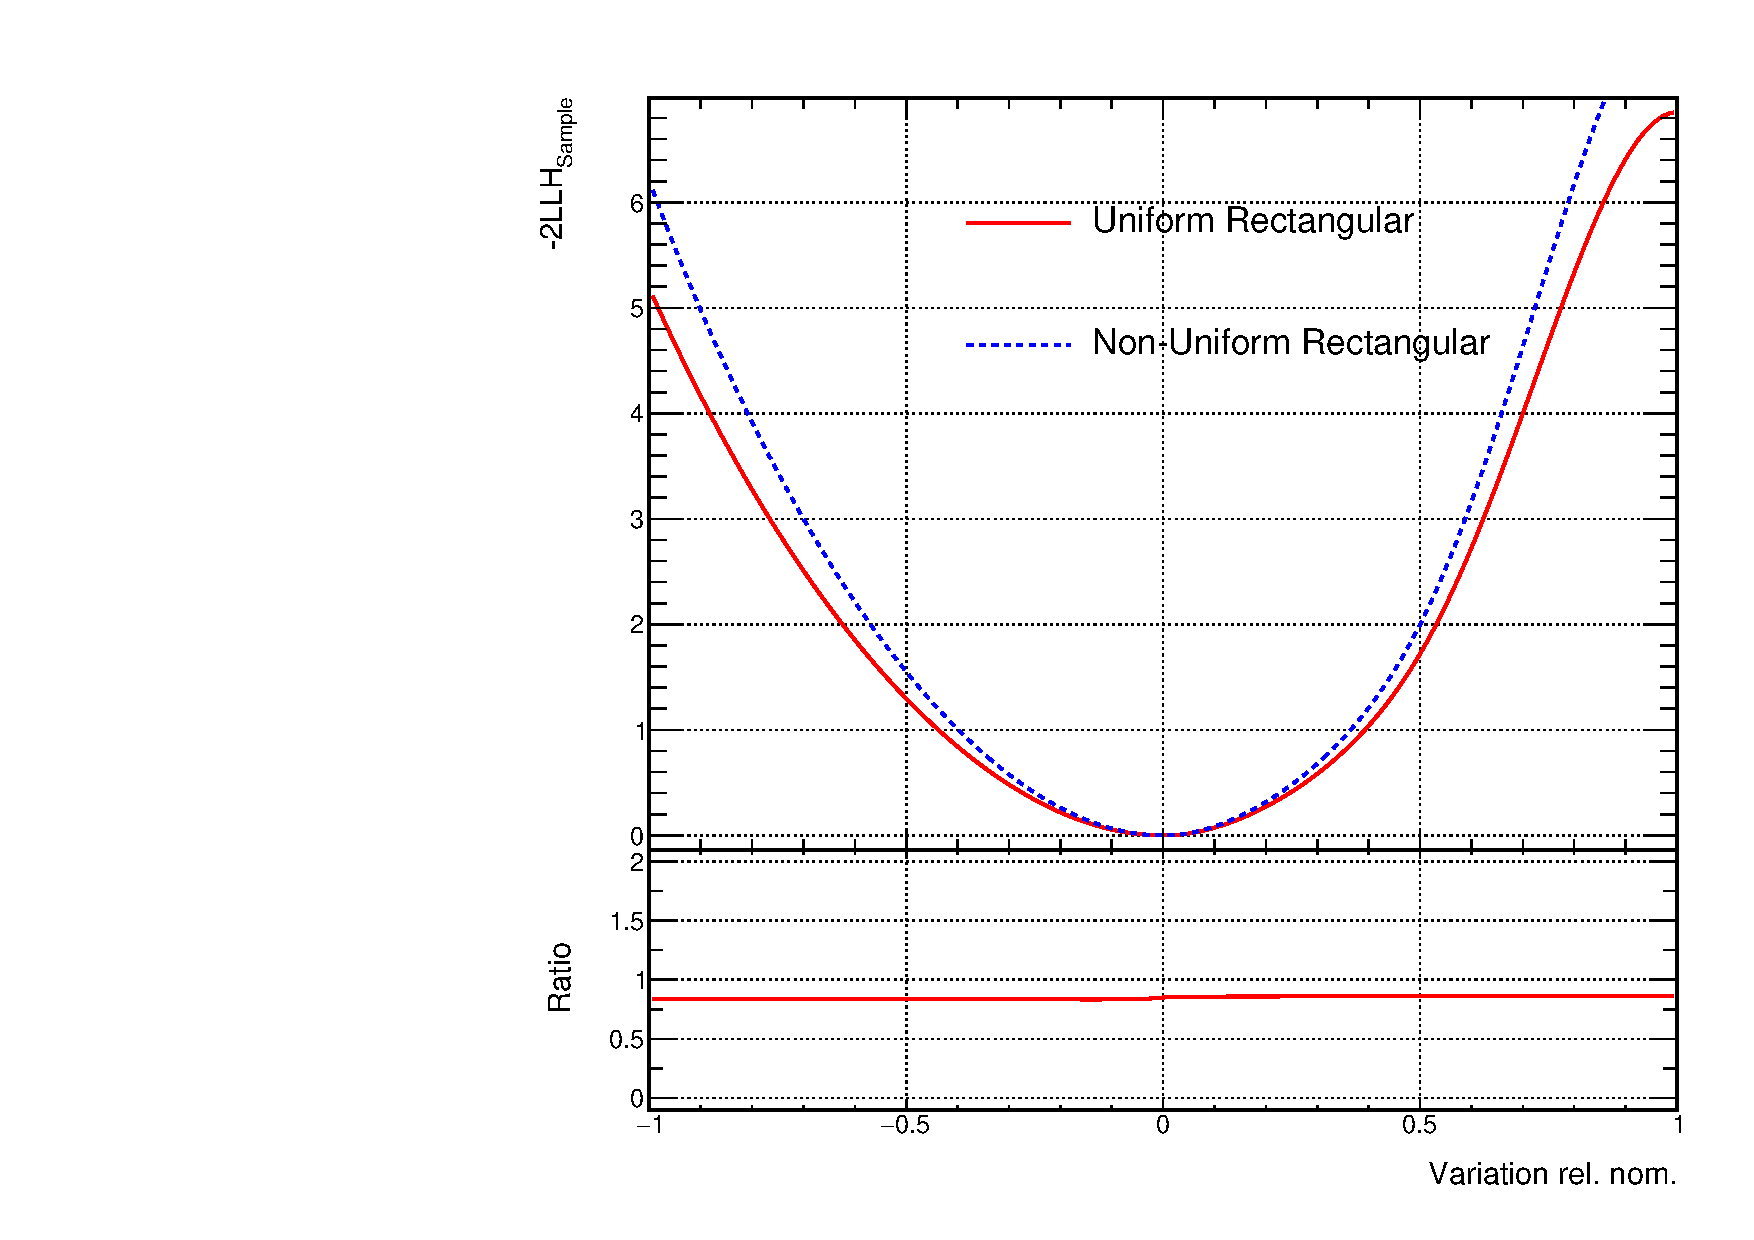
\includegraphics[width=0.95\linewidth]{figs/2p2h_shape_O_sampolyLLH}
  \caption{2p2h Shape $^{16}O$}
  \label{fig:2p2h_shape_O_sampolyLLH}
\end{subfigure}
\begin{subfigure}{.49\textwidth}
  \centering
  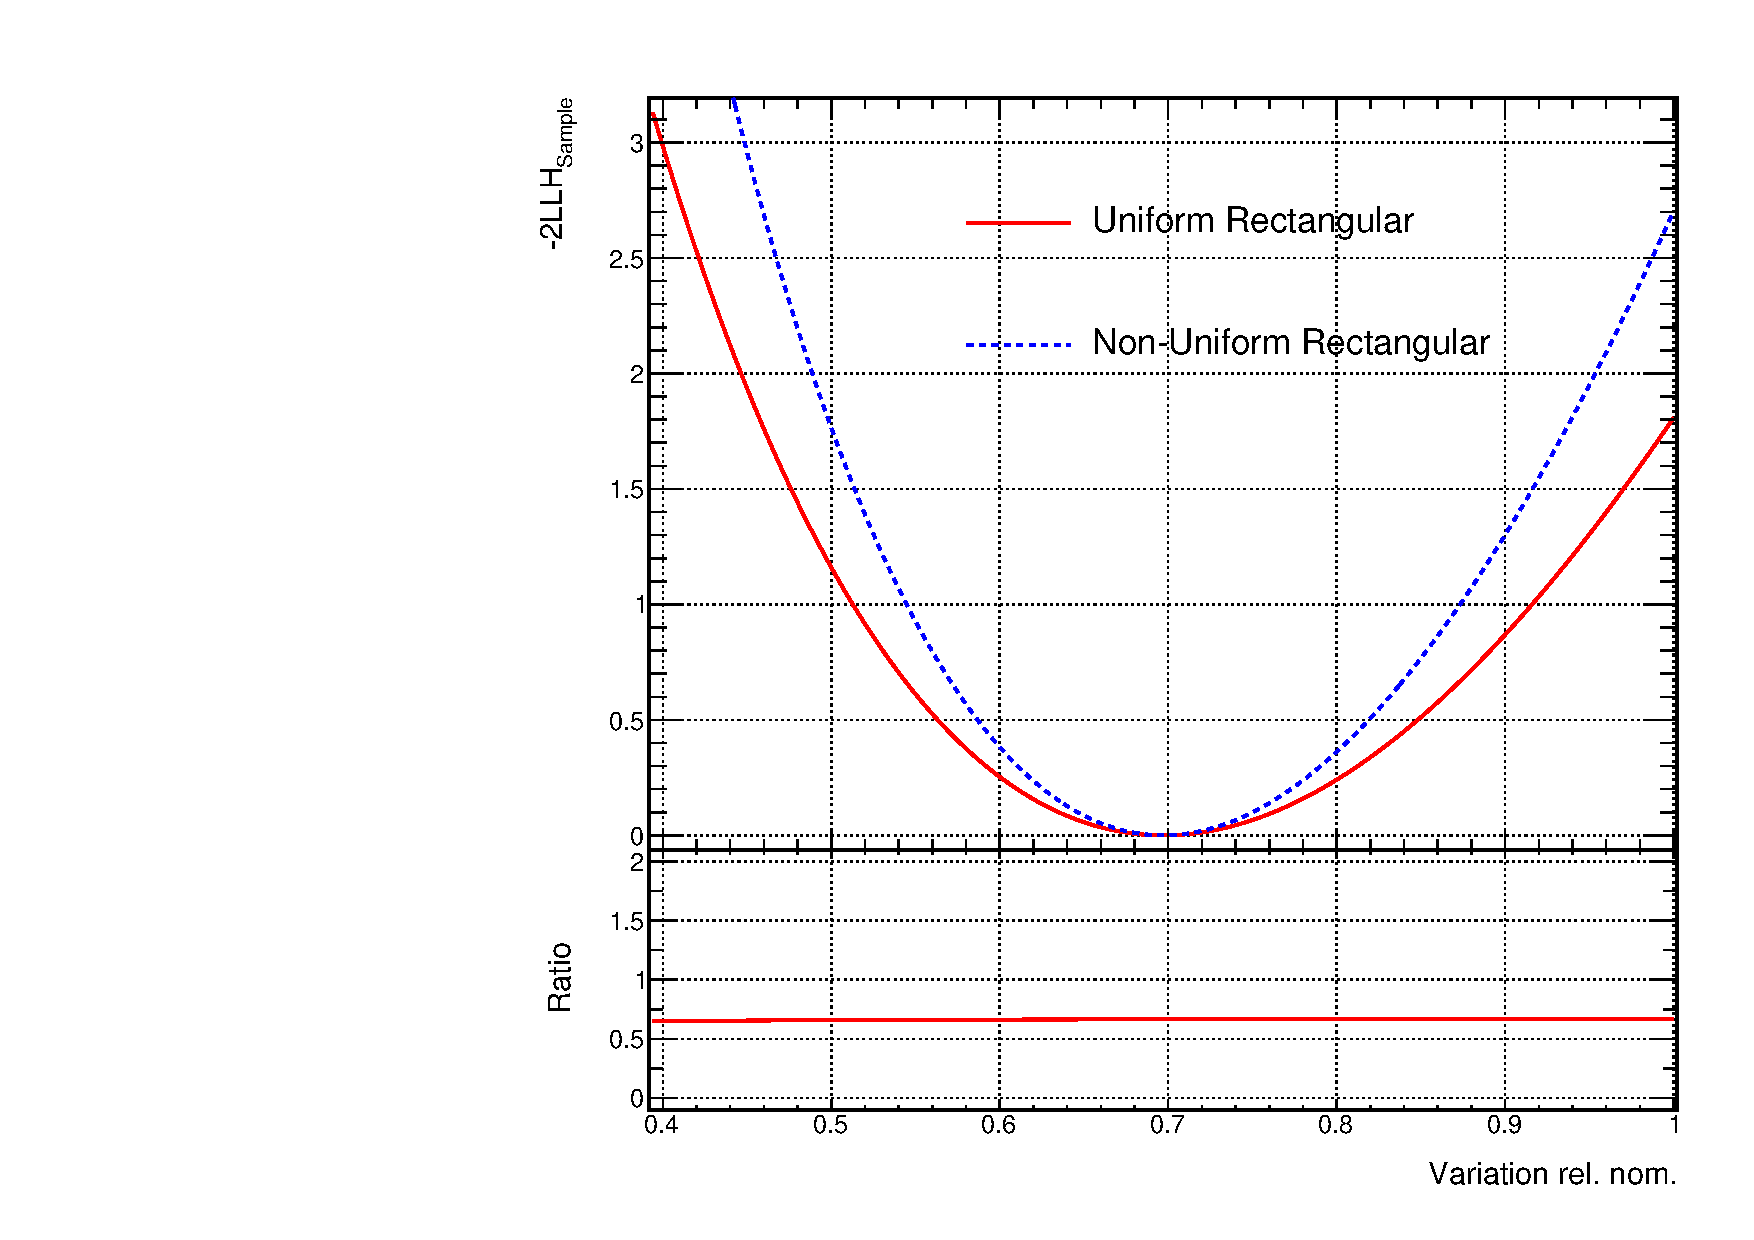
\includegraphics[width=0.95\linewidth]{figs/FEFCX_sampolyLLH}
  \caption{Pion FSI Single Charge Exchange}
  \label{fig:FEFCX_sampolyLLH}
\end{subfigure}
\begin{subfigure}{.49\textwidth}
  \centering
  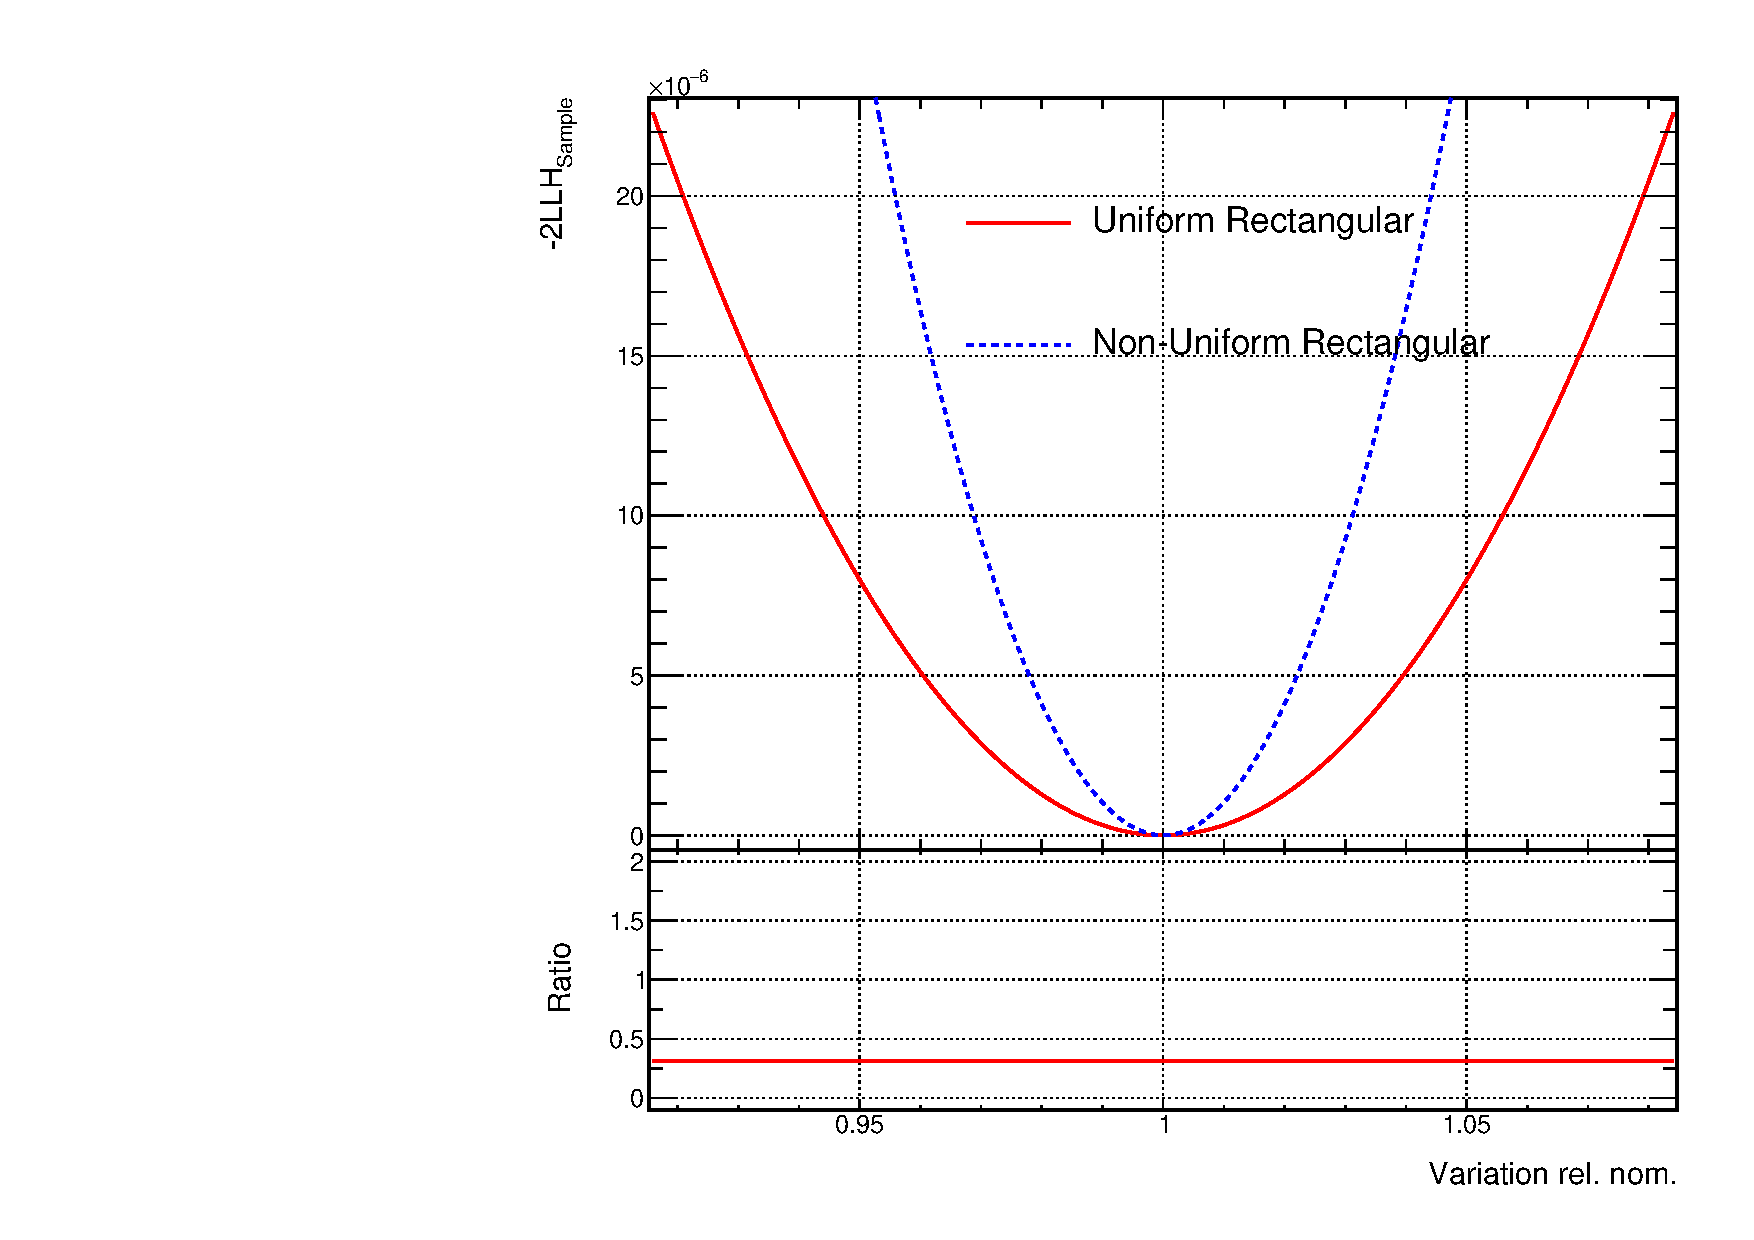
\includegraphics[width=0.95\linewidth]{figs/b_18_sampolyLLH}
  \caption{ND RHC $\nu_{\mu}$ 2500-30000 MeV Flux}
  \label{fig:b_30_sampolyLLH}
\end{subfigure}
\begin{subfigure}{.49\textwidth}
  \centering
  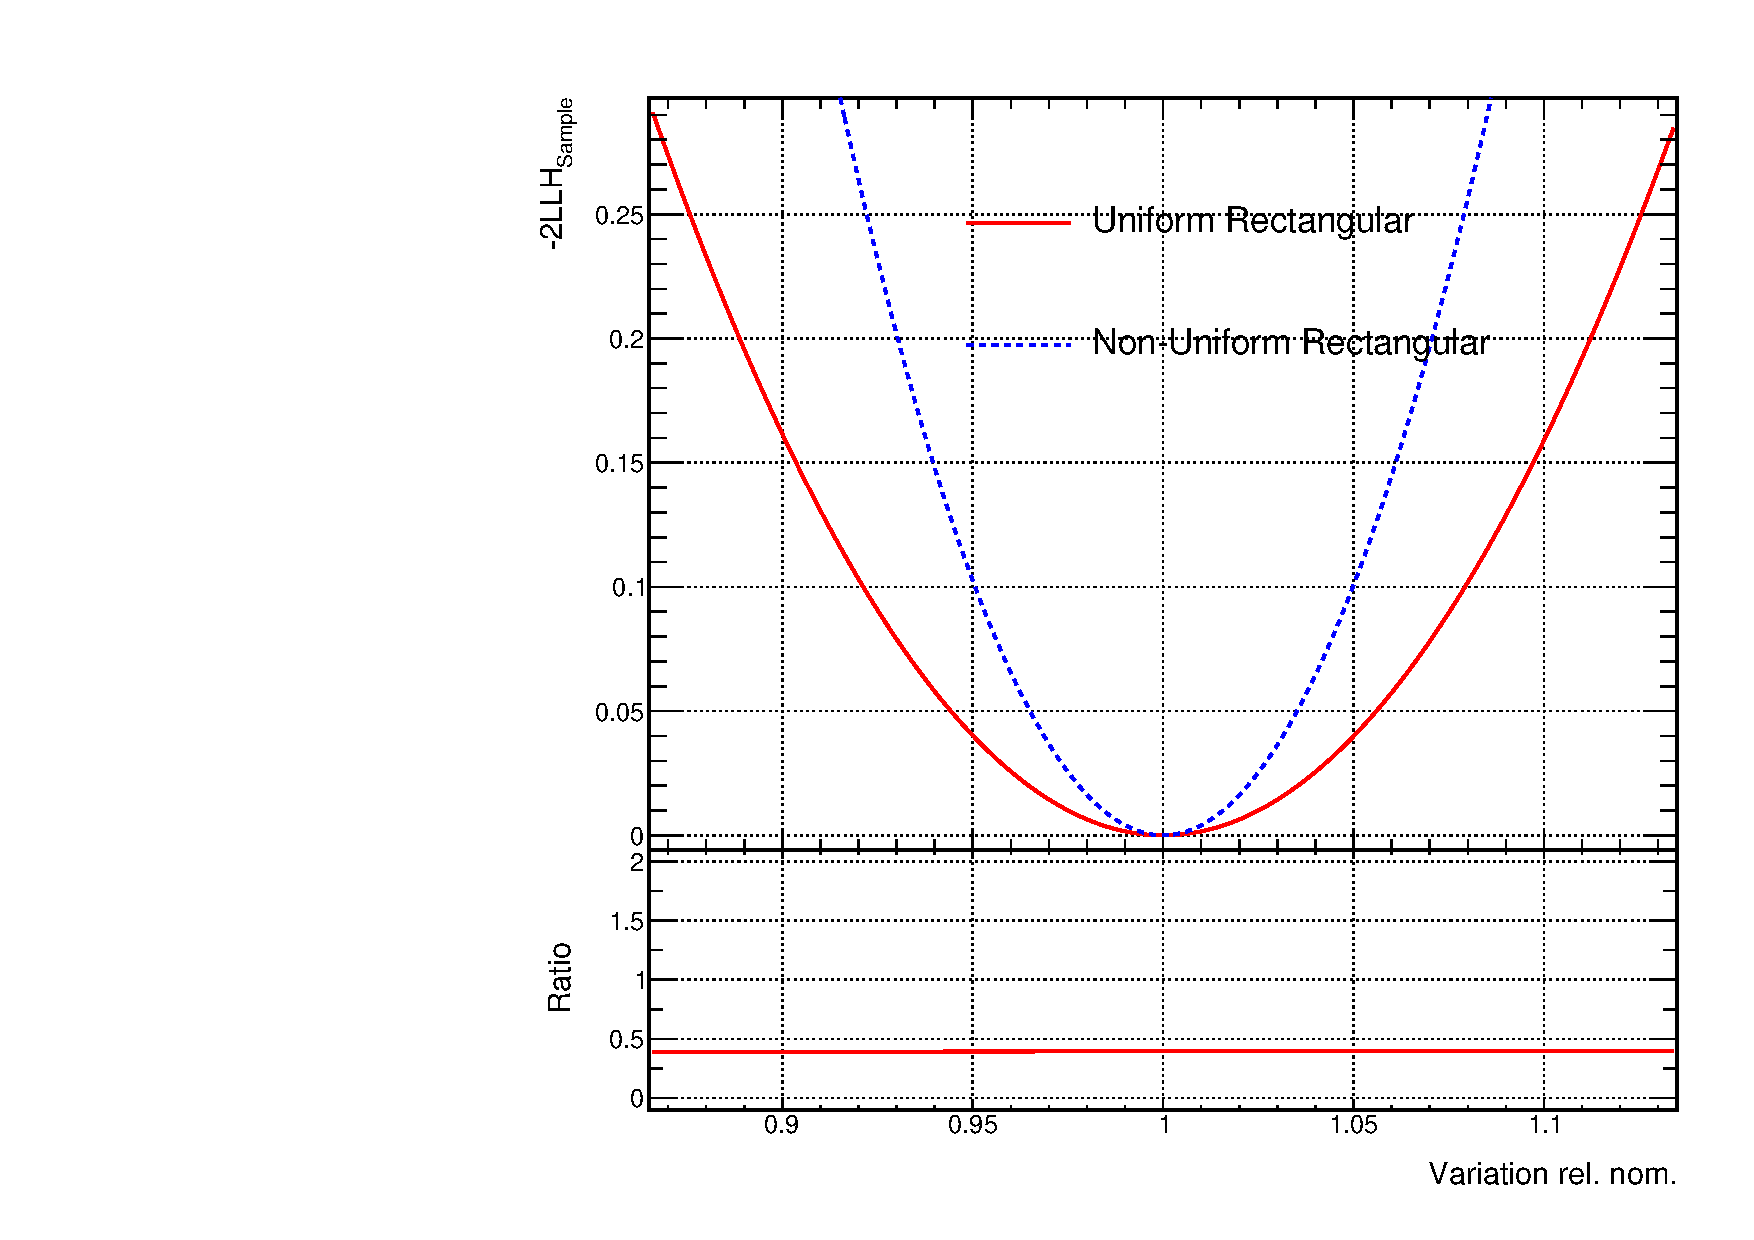
\includegraphics[width=0.95\linewidth]{figs/b_40_sampolyLLH}
  \caption{ND RHC $\bar{\nu_{e}}$ 1500-2500 MeV Flux}
  \label{fig:b_40_sampolyLLH}
\end{subfigure}
\caption{Comparison of LLH scans using uniform and non-uniform rectangular fit binning, for two selected interaction and beam parameters.}
\label{fig:polyllhscans}
\end{figure}


\section{Systematics}\label{sec:syst}

The purpose of the near detector fit is to constrain systematic uncertainties so that accurate oscillation measurements can be made at the far detector. It is therefore vital that these systematics are understood. 

In the near detector analysis, there are three sources of systematic uncertainties: 

\begin{itemize}

\item \textbf{Interaction: } Systematics from uncertainties on neutrino interaction cross-sections.

\item \textbf{Flux: } Systematics from uncertainties on the neutrino beam flux.

\item \textbf{Detector: } Systematics from uncertainties on the ND280 detector response and reconstruction.

\end{itemize}

The models of these three groups of systematics are parametrised, and each enter the fit through a covariance matrix. As a parameter is pulled from its prior value, a penalty is added to the likelihood, as shown in Equation \ref{eqn:systllh}. For systematics that are known to be constrained from external data, the likelihood penalty takes the form of a Gaussian. If there is no, or conflicting, data about a systematic, the likelihood penalty is just a constant. This is referred to as a `flat' prior uncertainty.

\subsection{Interaction}\label{sec:xsec}

The MC prediction is produced using the NEUT 5.4.0 generator\cite{neut}, as discussed in Section \ref{sec:ndsim}. The model for each interaction mode is therefore based on the models implemented in NEUT, with several modifications to tune to external data and additional theoretical calculations.

The uncertainties of these models are applied to the interaction modes they correspond to on an event by event basis. They are each parametrised as either shape or normalisation uncertainties. For normalisation parameters, the weight applied to the event is just the value of the parameter. However, for shape parameters, the weight applied at different values of the parameter depends on the kinematic variables of the event. Splines\footnote{The ROOT TSpline3 class is used here.} are used to translate from a change in parameter to a change in weight. These are produced by evaluating the change in weight for an event at evenly spaced values of the parameter, and interpolating between them. 

The parametrisation for each interaction mode proceeds using the following models:

\begin{itemize}

\item \textbf{CC Quasi-Elastic:}\\
The nominal MC is generated using a Spectral Function (SF) nuclear model from \cite{benhar}. There is one splined parameter, $M^{QE}_{A}$, for the axial mass in the dipole form factor. It's prior is informed by bubble chamber data\cite{tn344}. 

There are also eight normalisation parameters applied, for different bins in $Q^2$. The lowest five have width $0.05$ GeV$^2$, from $0.00$ GeV$^2$ up to $0.25$ GeV$^2$. The highest three span the ranges from $0.25$-$0.50$ GeV$^2$, $0.50$-$1.00$ GeV$^2$, and $>1.00$ GeV$^2$. Their prior central values and uncertainties are tuned by MINER$\nu$A \cite{minerva} data. 

The neutrino energy of CCQE events is calculated using Equation \ref{eqn:erec}, which is highly dependent on having an accurate value of the binding energy of the target nuclei. Four parameters are used to fit the binding energies (for target $^{12}$C/$^{16}$O and $\nu/\bar{\nu}$). These are neither shape nor normalisation parameters, and are described in more detail in Section \ref{sec:eb}.

\item \textbf{2-particle-2-hole:}\\
2p2h interactions are generated in NEUT using the Nieves model \cite{Nieves}. Two shape parameters apply to 2p2h interactions, one for events on $^{12}$C and one for events on $^{16}$O.  At one extreme it is entirely non-pionless-$\Delta$-decay-like in accordance with the Nieves model, and at the other extreme the shape is entirely pionless-$\Delta$-decay-like, in accordance with the Martini model\cite{Martini}. These two shape parameters have a 30$\%$ correlation.

There are additional shape parameters, to account for differences in the energy dependence of 2p2h interactions. At one extreme the shape is entirely consistent with the Nieves model, and at the other it is consistent with the Martini model. There are 4 of these parameters in total: $\nu/\bar{\nu}$ and high/low $E_{\nu}$. However, studies showed these could not be constrained using near detector data alone, so are fixed in near detector only fits. For the joint near and far detector fits in the oscillation analysis, the parameters are free in the fit. 

Three normalisations are also applied, one for $\nu$ events, one for $\bar{\nu}$, and one for $^{12}$C $\rightarrow ^{16}$O scaling. The latter is applied to events on $^{16}$O multiplicatively with the other normalisations.

\item \textbf{CC Resonance:}\\
The Rein-Sehgal model\cite{reinessehgal} is used to describe resonant $\pi$ production in NEUT. Splines are used to parametrise the resonance axial mass, $M^{Res}_{A}$, the normalisation of the axial form factor, $C^{A}_{5}$, and the size of the $I=1/2$ non-resonant background to $I=3/2$ resonant $\pi$ production. The prior central values and uncertainties are tuned using bubble chamber data \cite{bubblechamber}. There is a prior anti-correlation of 83$\%$ between $M^{Res}_{A}$ and $C^{A}_{5}$, 1$\%$ between $M^{Res}_{A}$ and $I=1/2$, and 31$\%$ between $C^{A}_{5}$ and $I=1/2$. In the joint near and far detector fits, the $I=1/2$ parameter is split into two, one for anti-neutrino events with $p_{\pi} < 200$ MeV, and one for all other $I=1/2$ non-resonant background events. In the near detector only fit, the low $p_{\pi}$ parameter is not fit, and the other $I=1/2$ parameter applies to all $I=1/2$ non-resonant background events.

\item \textbf{CC Coherent Scattering:}\\
The Rein-Seghal model \cite{reincoh} is used to describe coherent scattering events.
However, measurements at MINER$\nu$A show a $30\%$ difference in cross-section from this model. Two normalisation parameters are fit, one for CC events on $^{12}$C and one for CC events on $^{16}$O, each with a $30\%$ prior uncertainty to account for this discrepancy. These are $100\%$ correlated.

\item \textbf{CC Deep Inelastic Scattering and Multi-$\pi$:}\\
The CC DIS and multi-$\pi$ cross-section is calculated from `Structure Functions' of the nucleus, which themselves are constructed using `Parton Distribution Functions' (PDFs). The PDFs describe the probability of finding a quark with a given fraction of the nucleon momentum inside the nucleon. In NEUT, these are constructed using the GRV98\cite{grv98} model with corrections from Bodek and Yang\cite{by}. Two shape parameters are applied, one for DIS and one for multi-$\pi$ events, to account for uncertainty in the reliability of these corrections. One extreme corresponds to fully applying the corrections, and the other corresponds to not applying them at all.

Another shape parameter is applied to multi-$\pi$ events, to account for differences in the $\pi$ multiplicity models in different generators. If the $\pi$ multiplicity model changes, this directly alters the multi-$\pi$ cross-section (as it is required multi-$\pi$ events contain $\geq2$ $\pi$s). At one extreme, the multi-$\pi$ cross-section is entirely reweighted to the AGKY model\cite{agky} which has a smooth transition between low and high $W^2$ parametrisations, and at the other extreme it is entirely the nominal custom model in NEUT which has a hard cut-off between high and low $W^2$ parametrisations.

Two normalisation parameters are applied to CC DIS and multi-$\pi$ events, one for $\nu$ and one for $\bar{\nu}$ interactions. This is to account for a difference between the high energy CC-inclusive cross-sections in NEUT and the PDG world average. The prior uncertainty is $3.5\%$ for $\nu$ and $6.5\%$ for $\bar{\nu}$.

\item \textbf{CC Miscellaneous:}\\
A normalisation parameter with 100$\%$ uncertainty is applied to CC 1$K$, $1\eta$, and $1\gamma$ events.

\item \textbf{CC Inclusive:}\\
Two normalisations are applied to CC interactions with $0.4 < E_{\nu} < 0.6$ GeV, one for $\nu$ and one for $\bar{\nu}$ events. This is to account for the fact that the relative effect of the Coulomb corrections, described in Section \ref{sec:corr}, is smaller at higher momentum. The uncertainties on these systematics are $2\%$ and $1\%$ for $\nu$ and $\bar{\nu}$ respectively, and they are $100\%$ correlated.

\item \textbf{Neutral Current:}\\
As for CC Coherent scattering, NC scattering events receive a normalisation with $30\%$ uncertainty. NC $1\gamma$ interactions are modelled with the Rein-Sehgal CC Res model. The cross-section is half the value calculated with more recent models\cite{NCxsec}, and so the prior weight applied is 2.0. As there is no external data to constrain the cross-section, the prior uncertainty is $100\%$ of the nominal weight.

NC $\pi$ production is simulated using the same Rein-Sehgal model as for CC $\pi$ production, and the same parameters are applied: $C^{A}_{5}$, $M^{Res}_{A}$ and $I=1/2$.

NC DIS, multi-$\pi$, $1\eta$, and $1K$ are grouped together and receive the same normalisation parameter (NC Other), with a $30\%$ uncertainty. In the full joint analysis, separate NC Other parameters are applied to near and far detector events.

\item \textbf{Electron (Anti-)Neutrino:}\\
As all the other systematic uncertainties are determined for $\nu_{\mu}$ or $\bar{\nu_{\mu}}$ interactions, a normalisation is applied to all $\nu_{e}$ and $\bar{\nu_{e}}$ events. This is to account for any unmodelled effects which affect $\nu_{e}$/$\bar{\nu_{e}}$ events but not $\nu_{\mu}$/$\bar{\nu_{\mu}}$. As these processes may be different for neutrinos and anti-neutrinos, there are two normalisations, one for $\nu_{e}$ and one for $\bar{\nu_{e}}$. The prior uncertainty is $2.8\%$ and the two parameters are $50\%$ anti-correlated, as calculated in \cite{nuenuebar}.

\item \textbf{Final State Interactions:} \\
The propagation of $\pi$s produced in neutrino interactions is simulated as a cascade implementation of the model described in \cite{fsicascade}. There are five shape parameters representing the probability of different interactions at each step in the cascade. The 5 types of final state interaction parametrised are quasi-elastic scattering (at low and high energy), $\pi$ production, $\pi$ absorption, and charge exchange. The prior central values and uncertainties are tuned to $\pi$-nucleon scattering data\cite{fsiscatt}.

When nucleon final state interactions produce $\pi$s, the $\pi$s are propagated with the above systematics. However, nucleon final state interactions are not accounted for in the MC.

\end{itemize}

A summary of the interaction parameters is shown in Table \ref{tab:xsecparams}. The full prefit cross-section correlation matrix is shown in Figure \ref{fig:xseccov}, showing the central values, uncertainties, and correlations of the parameters described in this section.

\begin{center}
\begin{table}
\begin{adjustwidth}{-.9in}{-.9in}
\centering
\scalebox{0.85}{
\begin{tabular}{ c||c|c|c|c|c} 
\hline
\hline
 \textbf{Parameter} & \textbf{Events} & \addstackgap{\shortstack{\textbf{Prior (Nominal)} \\ \textbf{Central Value}}} & \shortstack{\textbf{Prior} \\ \textbf{Uncertainty}} & \shortstack{\textbf{Prior} \\ \textbf{Shape}} & \textbf{Type}\\
\hline
\hline
\textbf{$M^{QE}_{A}$} & CCQE & 1.03 (1.21) GeV & 0.06 GeV & Gaus & Shape\\
\hline
\textbf{2p2h Norm $\nu$} & 2p2h, $\nu$ & 1.0 & 1.0 & Flat & Norm.\\
\hline
\textbf{2p2h Norm $\bar{\nu}$} & 2p2h, $\bar{\nu}$ & 1.0 & 1.0 & Flat & Norm.\\
\hline
\textbf{2p2h Norm $^{12}$C to $^{16}$O} & 2p2h on $^{16}$O & 1.0 & 0.2 & Gaus & Norm.\\
\hline
\textbf{2p2h Shape $^{12}$C} & 2p2h on $^{12}$C & 1.0 & 3.0 & Gaus & Shape\\
\hline
\textbf{2p2h Shape $^{16}$O} & 2p2h on$^{16}$O & 1.0 & 3.0 & Gaus & Shape\\
\hline
\textbf{2p2h E dep low E $\nu$} & - & - & - & - & -\\
\hline
\textbf{2p2h E dep high E $\nu$} & - & - & - & - & -\\
\hline
\textbf{2p2h E dep low E $\bar{\nu}$} & - & - & - & - & -\\
\hline
\textbf{2p2h E dep high E $\bar{\nu}$} & - & - & - & - & -\\
\hline
\textbf{$Q^2$ 0} & CCQE; $0.0<Q^{2}<0.05$ GeV$^{2}$ & 0.495 (1.0) & 1.0 & Flat & Norm. \\
\hline
\textbf{$Q^2$ 1} & CCQE; $0.05<Q^{2}<0.10$ GeV$^{2}$ & 0.695 (1.0) & 1.0 & Flat & Norm. \\
\hline
\textbf{$Q^2$ 2} & CCQE; $0.1<Q^{2}<0.15$ GeV$^{2}$& 0.78 (1.0) & 1.0 & Flat & Norm. \\
\hline
\textbf{$Q^2$ 3} & CCQE; $0.15<Q^{2}<0.2$ GeV$^{2}$ & 0.89 (1.0) & 1.0 & Flat & Norm. \\
\hline
\textbf{$Q^2$ 4} & CCQE; $0.2<Q^{2}<0.25$ GeV$^{2}$ & 0.93 (1.0) & 1.0 & Flat & Norm. \\
\hline
\textbf{$Q^2$ 5} & CCQE; $0.25<Q^{2}<0.5$ GeV$^{2}$ & 1.0 & 0.11 & Gaus & Norm.\\
\hline
\textbf{$Q^2$ 6} & CCQE; $0.5<Q^{2}<1.0$ GeV$^{2}$ & 1.0 & 0.18 & Gaus & Norm.\\
\hline
\textbf{$Q^2$ 7} & CCQE; $Q^{2}<1.0$ GeV$^{2}$ & 1.0 & 0.40 & Gaus & Norm.\\
\hline
\textbf{$E_{b} \nu$ C} & CCQE on $^{12}$C; $E_{\nu} < 4$ GeV; $\nu$ & 27 (25) MeV & 6 MeV & Gaus & $p_{\mu}$ Shift\\
\hline
\textbf{$E_{b} \bar{\nu}$ C} & CCQE on $^{12}$C; $E_{\nu} < 4$ GeV; $\bar{\nu}$ & 25 MeV & 6 MeV & Gaus & $p_{\mu}$ Shift\\
\hline
\textbf{$E_{b} \nu$ O} & CCQE on $^{16}$O; $E_{\nu} < 4$ GeV; $\nu$ & 31 (27) MeV & 6 MeV & Gaus & $p_{\mu}$ Shift\\
\hline
\textbf{$E_{b} \bar{\nu}$ O} & CCQE on $^{16}$O; $E_{\nu} < 4$ GeV; $\bar{\nu}$ & 27 MeV & 6 MeV & Gaus & $p_{\mu}$ Shift\\
\hline
\textbf{$M^{RES}_{A}$} & CC Res, NC $\pi^{0}$, NC $\pi^{\pm}$ & 1.07 (0.95) GeV & 0.15 GeV & Gaus & Shape\\
\hline
\textbf{$C^{A}_{5}$} & CC Res, NC $\pi^{0}$, NC $\pi^{\pm}$ & 0.96 (1.01) & 0.15 & Gaus & Shape\\
\hline
\textbf{$I_{1/2}$ non-res} & CC Res, NC $\pi^{0}$, NC $\pi^{\pm}$ & 0.96 (1.30) & 0.40 & Gaus & Shape\\
\hline
\textbf{$I_{1/2}$ non-res low $p_{\pi}$} & - & - & - & - & -\\
\hline
\textbf{CC norm $\nu$} & CC; $0.4 <E_{\nu} < 0.6$ GeV; $\nu$ & 1.0 & 0.02 & Gaus & Norm.\\
\hline
\textbf{CC norm $\bar{\nu}$} & CC; $0.4 <E_{\nu} < 0.6$ GeV; $\bar{\nu}$ & 1.0 & 0.01 & Gaus & Norm.\\
\hline
\textbf{CC $\nu_{e}$/$\nu_{\mu}$} & CC; $\nu_{e}$ & 1.0 & 0.028 & Gaus & Norm.\\
\hline
\textbf{CC $\bar{\nu_{e}}$/$\bar{\nu_{\mu}}$} & CC; $\bar{\nu_{e}}$ & 1.0 & 0.028 & Gaus & Norm.\\
\hline
\textbf{CC BY DIS} & CC DIS; $W<$ 4.0 GeV & 1.0 & 1.0 & Gaus & Shape\\
\hline
\textbf{CC BY multi-$\pi$} & CC multi-$\pi$; $1.6<W<2.0$ GeV & 1.0 & 1.0 & Gaus & Shape\\
\hline
\textbf{CC AGKY mult} & CC multi-$\pi$; $1.6<W<2.0$ GeV & 1.0 & 1.0 & Gaus & Shape\\
\hline
\textbf{CC misc} & CC$1\gamma$, CC1$K$, CC1$\eta$ & 1.0 & 1.0 & Gaus & Norm.\\
\hline
\textbf{CC DIS, multi-$\pi$ norm $\nu$} & CC DIS, CC multi-$\pi$, $\nu$ & 1.0 & 0.035 & Gaus & Norm.\\
\hline
\textbf{CC DIS, multi-$\pi$ norm $\bar{\nu}$} & CC DIS, CC multi-$\pi$, $\bar{\nu}$ & 1.0 & 0.065 & Gaus & Norm.\\
\hline
\textbf{CC coh$^{12}$C} & CC Coherent on $^{12}$C & 1.0 & 0.3 & Gaus & Norm.\\
\hline
\textbf{CC coh $^{16}$O} & CC Coherent on $^{16}$O & 1.0 & 0.3 &  Gaus & Norm.\\
\hline
\textbf{NC coh} & NC Coherent & 1.0 & 0.3 & Gaus & Norm.\\
\hline
\textbf{NC 1$\gamma$} & NC 1$\gamma$ & 1.0 & 1.0 & Gaus & Norm.\\
\hline
\textbf{NC other near} & NC DIS, multi-$\pi$, $1K$, $1\eta$ & 1.0 & 0.3 & Gaus & Norm.\\
\hline
\textbf{NC other far} & - & - & - & - & -\\
\hline
\textbf{$\pi$ FSI QE} & CC Res, NC $\pi^{0}$, NC $\pi^{\pm}$ & 1.069 & 0.313 & Gaus & Shape\\
\hline
\textbf{$\pi$ FSI QE high E} & CC Res, NC $\pi^{0}$, NC $\pi^{\pm}$ & 1.824 & 0.859 & Gaus & Shape\\
\hline
\textbf{$\pi$ FSI Abs} &  CC Res, NC $\pi^{0}$, NC $\pi^{\pm}$ & 1.002 & 1.102 & Gaus & Shape\\
\hline
\textbf{$\pi$ FSI Prod} & CC Res, NC $\pi^{0}$, NC $\pi^{\pm}$ & 1.404 & 0.432 & Gaus & Shape\\
\hline
\textbf{$\pi$ FSI CX} &  CC Res, NC $\pi^{0}$, NC $\pi^{\pm}$ & 0.697 & 0.305 & Gaus & Shape\\
\hline
\hline
\end{tabular}}
\caption{The interaction parameters used in this analysis.}\label{tab:xsecparams}
\end{adjustwidth}
\end{table}
\end{center}

\begin{figure}[!htbp]
\centering
\includegraphics*[width=0.7\textwidth,clip]{figs/xseccorr}
\caption{The cross-section correlation matrix.}\label{fig:xseccov}
\end{figure}

\subsubsection{Binding Energy}\label{sec:eb}

The uncertainty on the binding energy was the largest individual systematic in the previous oscillation analysis. It contributed 3.7$\%$ to the uncertainty on the predicted relative number of electron neutrino and electron anti-neutrino candidates at SK (with no decay electrons)\cite{t2knature}. Studies of simulated datasets also showed that the uncertainty had a significant impact on the credible intervals of the measured oscillation parameters \cite{tn331}. To reduce its impact, a new treatment of the uncertainty was implemented for this analysis.

In the SF nuclear model, there isn't a single nuclear binding energy systematic uncertainty. Instead, external data is used to inform distributions of the nuclear binding energy and initial nucleon momentum, which contain peaks corresponding to the nuclear shell structure. The peaks are shown for different initial nucleon momentum for the ground state in Figure \ref{fig:sfshells}.

\begin{figure}[!htbp]
\centering
\includegraphics*[width=0.7\textwidth,clip]{figs/SFShells}
\caption{Removal energy (`$E$') at different values of the initial nucleon momentum (`k') for the ground state in the SF model. Figure from \cite{tn344}.}\label{fig:sfshells}
\end{figure}

Ideally, there would be systematic parameters for the height, width, and position of each of the peaks for each target nucleus. However, this was not feasible to implement on the time scale of this analysis. Instead, a global uncertainty of 6 MeV is applied to the removal energy in the SF nuclear model.

These binding energy systematics are implemented as neither shape nor normalisation parameters in the T2K oscillation analysis. Instead, the offset to the removal energy is propagated to a change in the $p_{\mu}-$cos$\theta_{\mu}$ distributions by directly shifting $p_{\mu}$. It has been shown that changes in the removal energy do not cause significant changes in the distribution of $\theta_{\mu}$\cite{tn344}.

The SF model used was constrained using data from $ee',p$ experiments, which only applies to initial state protons, and therefore anti-neutrino CCQE interactions. The spectral function of initial state neutrons in neutrino CCQE interactions can not be constrained in the same way. The offset between the SF and Relativistic Mean-Field model predictions \cite{RMFPred} for neutrons is $\sim$4 MeV for oxygen and $\sim$2 MeV for carbon. 

There are therefore four binding energy parameters applied to CCQE events: for $^{12}$C/$^{16}$O and $\nu$/$\bar{\nu}$. The $\bar{\nu}$ parameters have a prior central value of 25 MeV for $^{12}$C, and 27 MeV for $^{16}$O. The central value of the $\nu$ parameters are offset from their $\bar{\nu}$ counterparts by 2 and 4 MeV for $^{12}$C and $^{16}$O respectively. The parameters are correlated with each other as follows:

\begin{itemize}

\item \textbf{$E_{b}\nu$ O:} 70$\%$ with $E_{b}\bar{\nu}$ O, 77.77$\%$ with $E_{b}\nu$ C, 65.27$\%$ with $E_{b}\bar{\nu}$ C

\item \textbf{$E_{b}\bar{\nu}$ O:} 70$\%$ with $E_{b}\nu$ O, 65.27$\%$ with $E_{b}\nu$ C, 77.77$\%$ with $E_{b}\bar{\nu}$ C

\item \textbf{$E_{b}\nu$ C:} 77.77$\%$ with $E_{b}\nu$ O, 65.27$\%$ with $E_{b}\bar{\nu}$ O, 70$\%$ with $E_{b}\bar{\nu}$ C

\item \textbf{$E_{b}\bar{\nu}$ O:} 65.27$\%$ with $E_{b}\nu$ C, 77.77$\%$ with $E_{b}\bar{\nu}$ O, 70$\%$ with $E_{b}\nu$ C

\end{itemize}

These values are derived in \cite{tn344}.

The effect of the $E_b \nu$ C parameter on the FGD1 FHC CC0$\pi$ sample is shown in Figure \ref{fig:Ebratios}. Here, the parameter is set to $\pm1\sigma$ while all other parameters are kept at nominal, and the ratio to the nominal MC is taken. As the binding energy parameter is increased, the final state lepton momentum is decreased. This is seen in the increase in number of events at lower momentum in Figure \ref{fig:EbratiosP1}. The opposite effect is seen for decreasing the binding energy parameter in Figure \ref{fig:EbratiosM1}.

\begin{figure}
\centering
\begin{subfigure}{.5\textwidth}
  \centering
  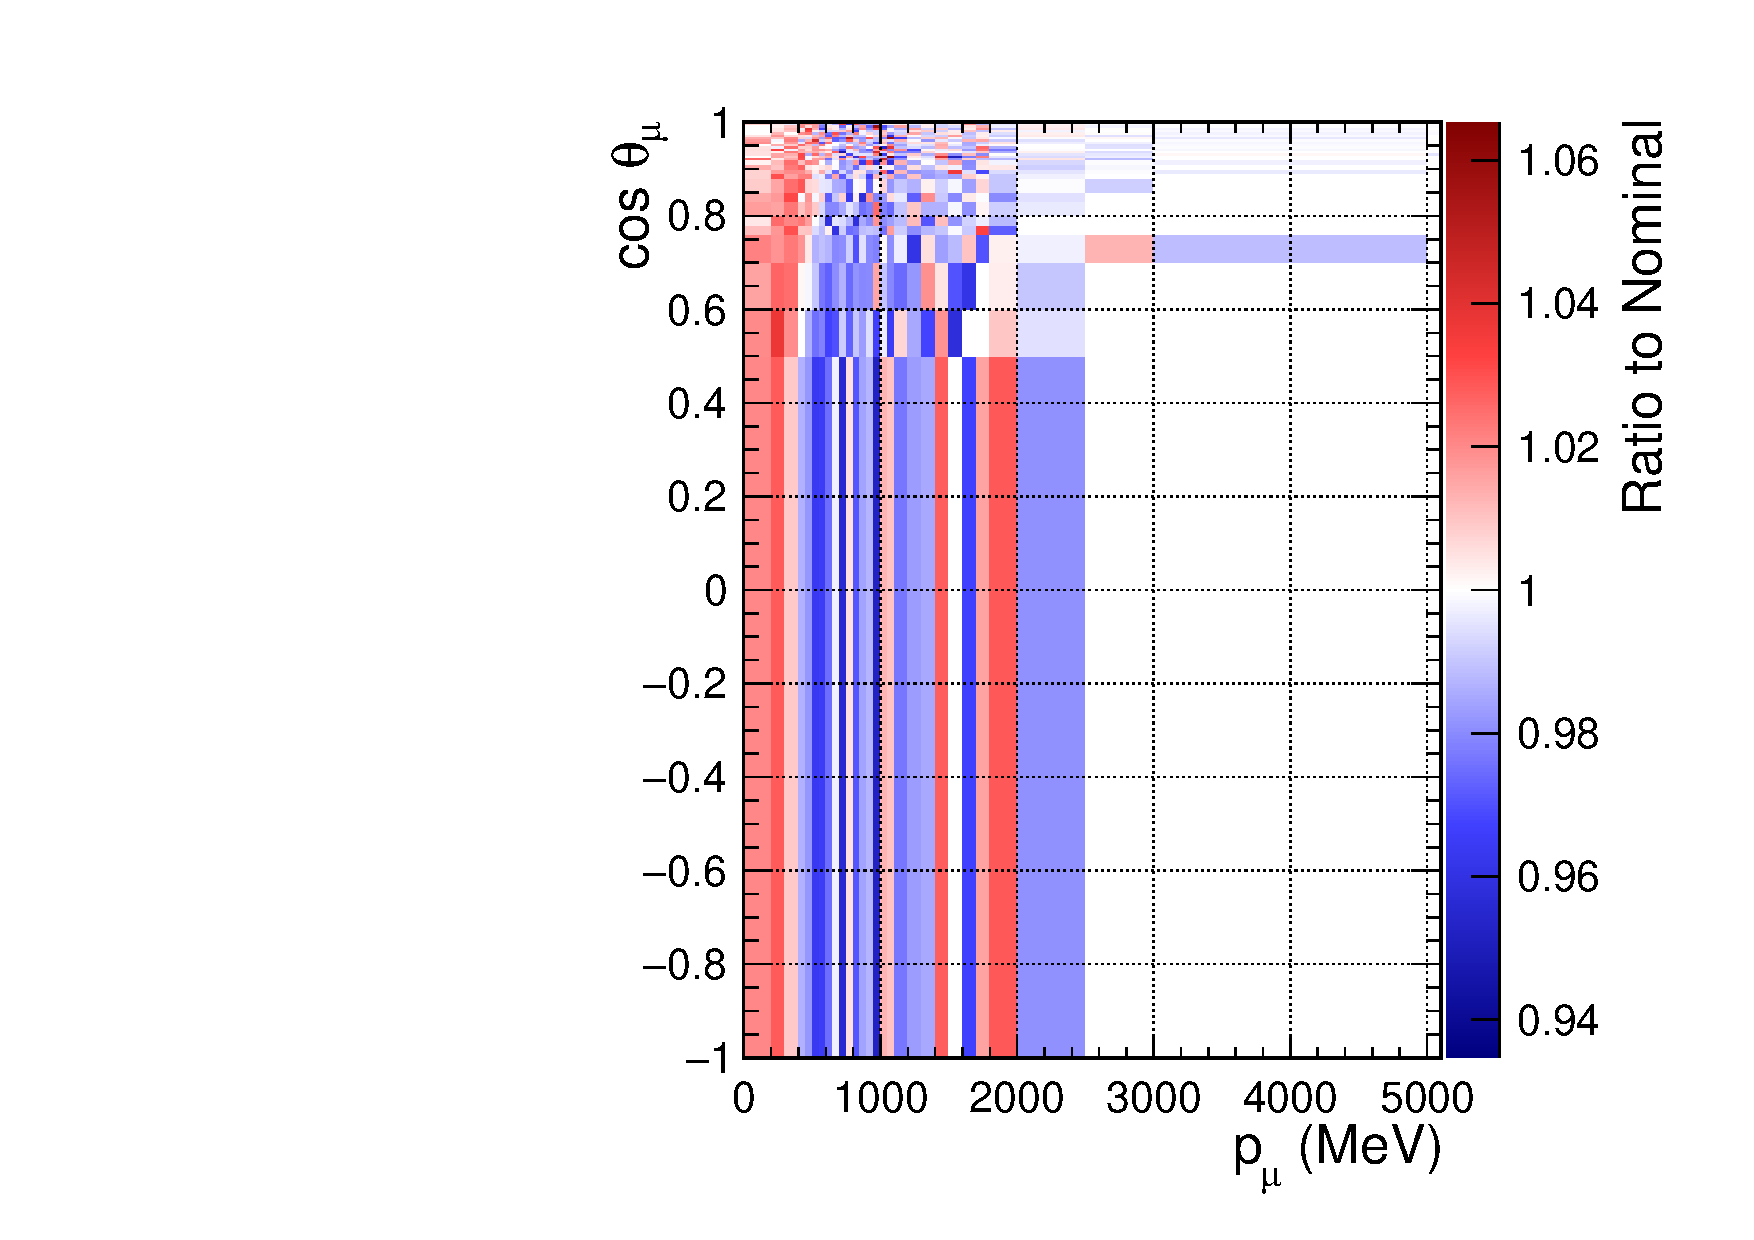
\includegraphics[width=0.95\linewidth]{figs/EbNuCP1Ratio}
  \caption{$+1\sigma$}\label{fig:EbratiosP1}
\end{subfigure}%
\begin{subfigure}{.5\textwidth}
  \centering
  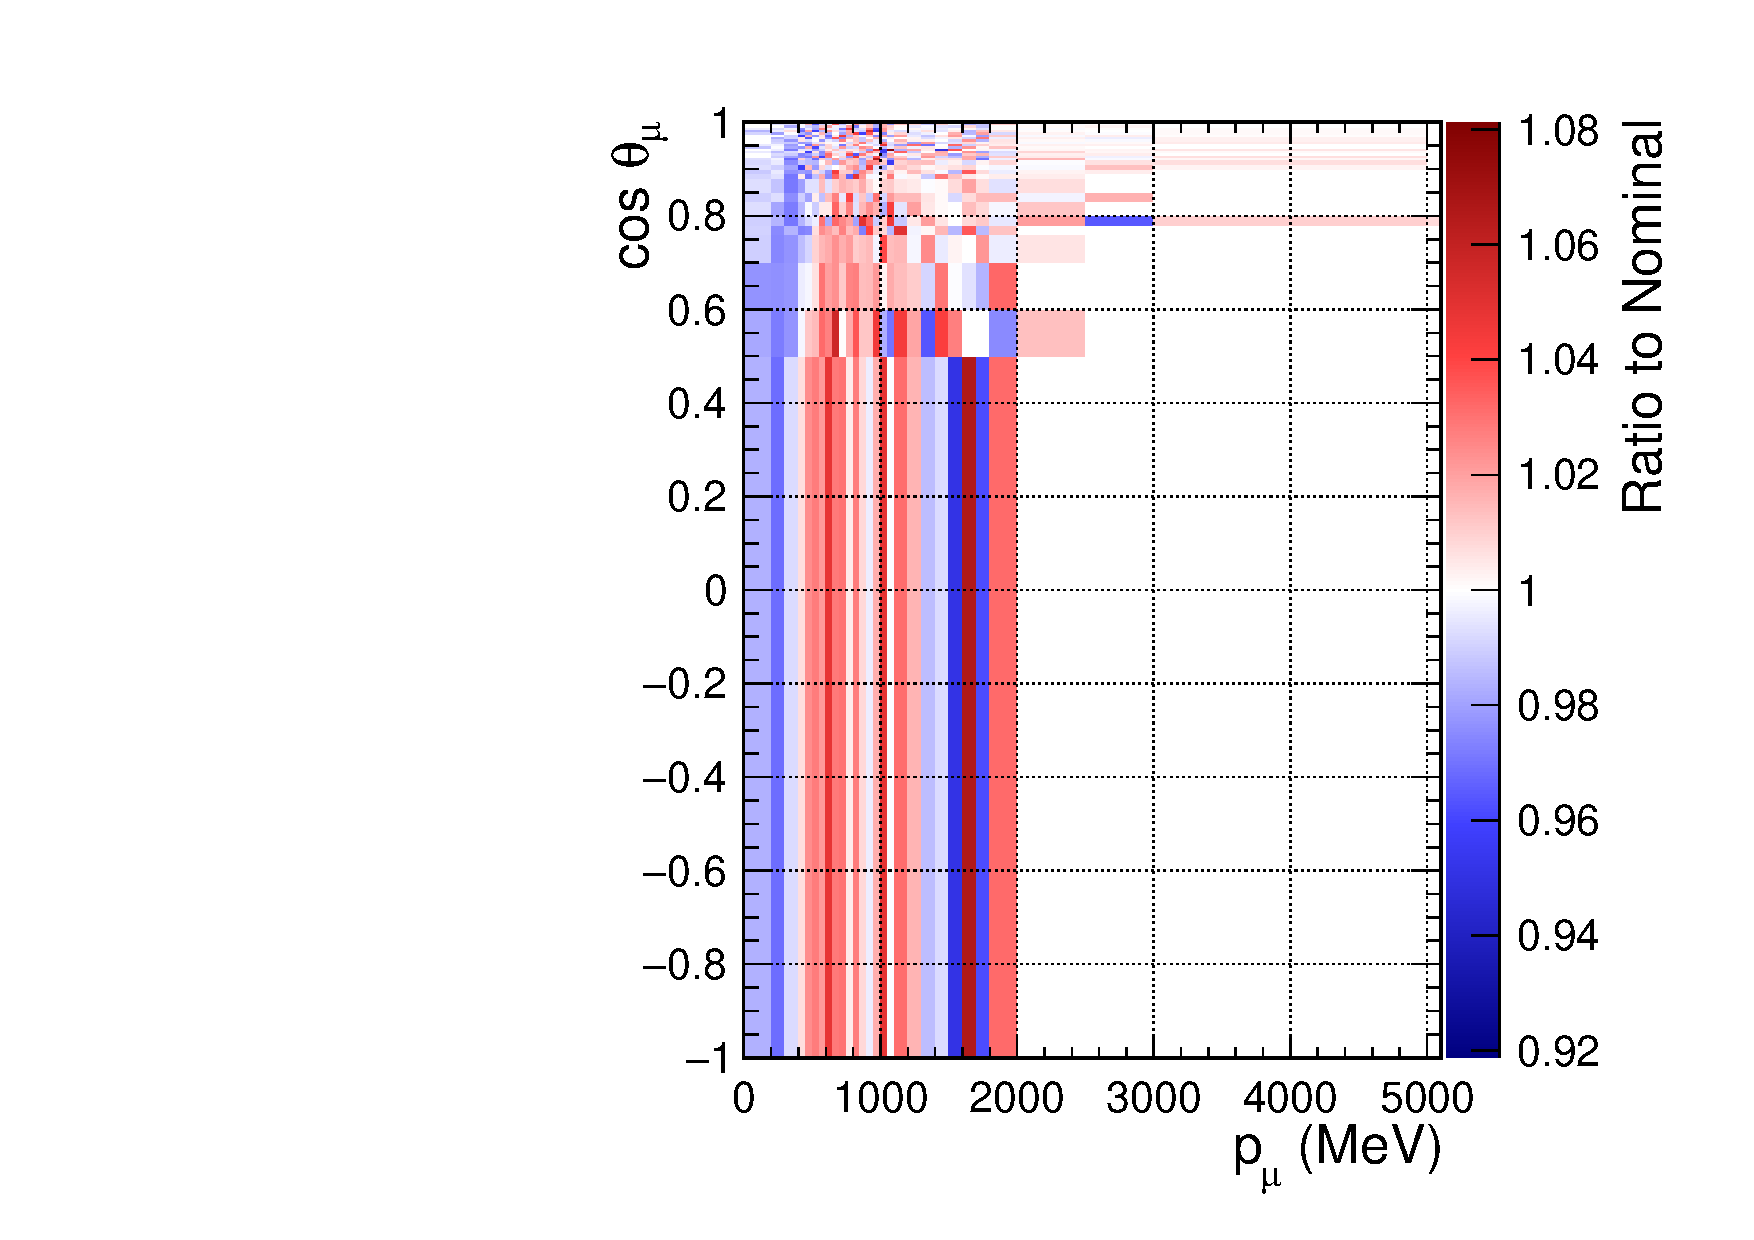
\includegraphics[width=0.95\linewidth]{figs/EbNuCM1Ratio}
  \caption{$-1\sigma$}\label{fig:EbratiosM1}
\end{subfigure}
\caption{Ratio of the FGD1 FHC CC0$\pi$ sample with $E_{b}\nu$ C parameter set to $\pm 1\sigma$ to the nominal MC.}
\label{fig:Ebratios}
\end{figure}

To validate the implementation of this new type of parameter, Asimov fits\cite{asmv} (where the nominal MC is fitted to itself) with binding energy included were run. The Asimov fitting process is described in more detail in Section \ref{sec:asimov}. The 1D posterior distributions for each of the 4 parameters are shown in Figure \ref{fig:Ebasimov}, with a fitted Gaussian distribution. These validations were performed using the uniform binning described in Appendix \ref{app:bintemplates}. As expected, the postfit values are close to the nominal values, and the distributions are approximately Gaussian. 

\begin{figure}
\centering
\begin{subfigure}{.48\textwidth}
  \centering
  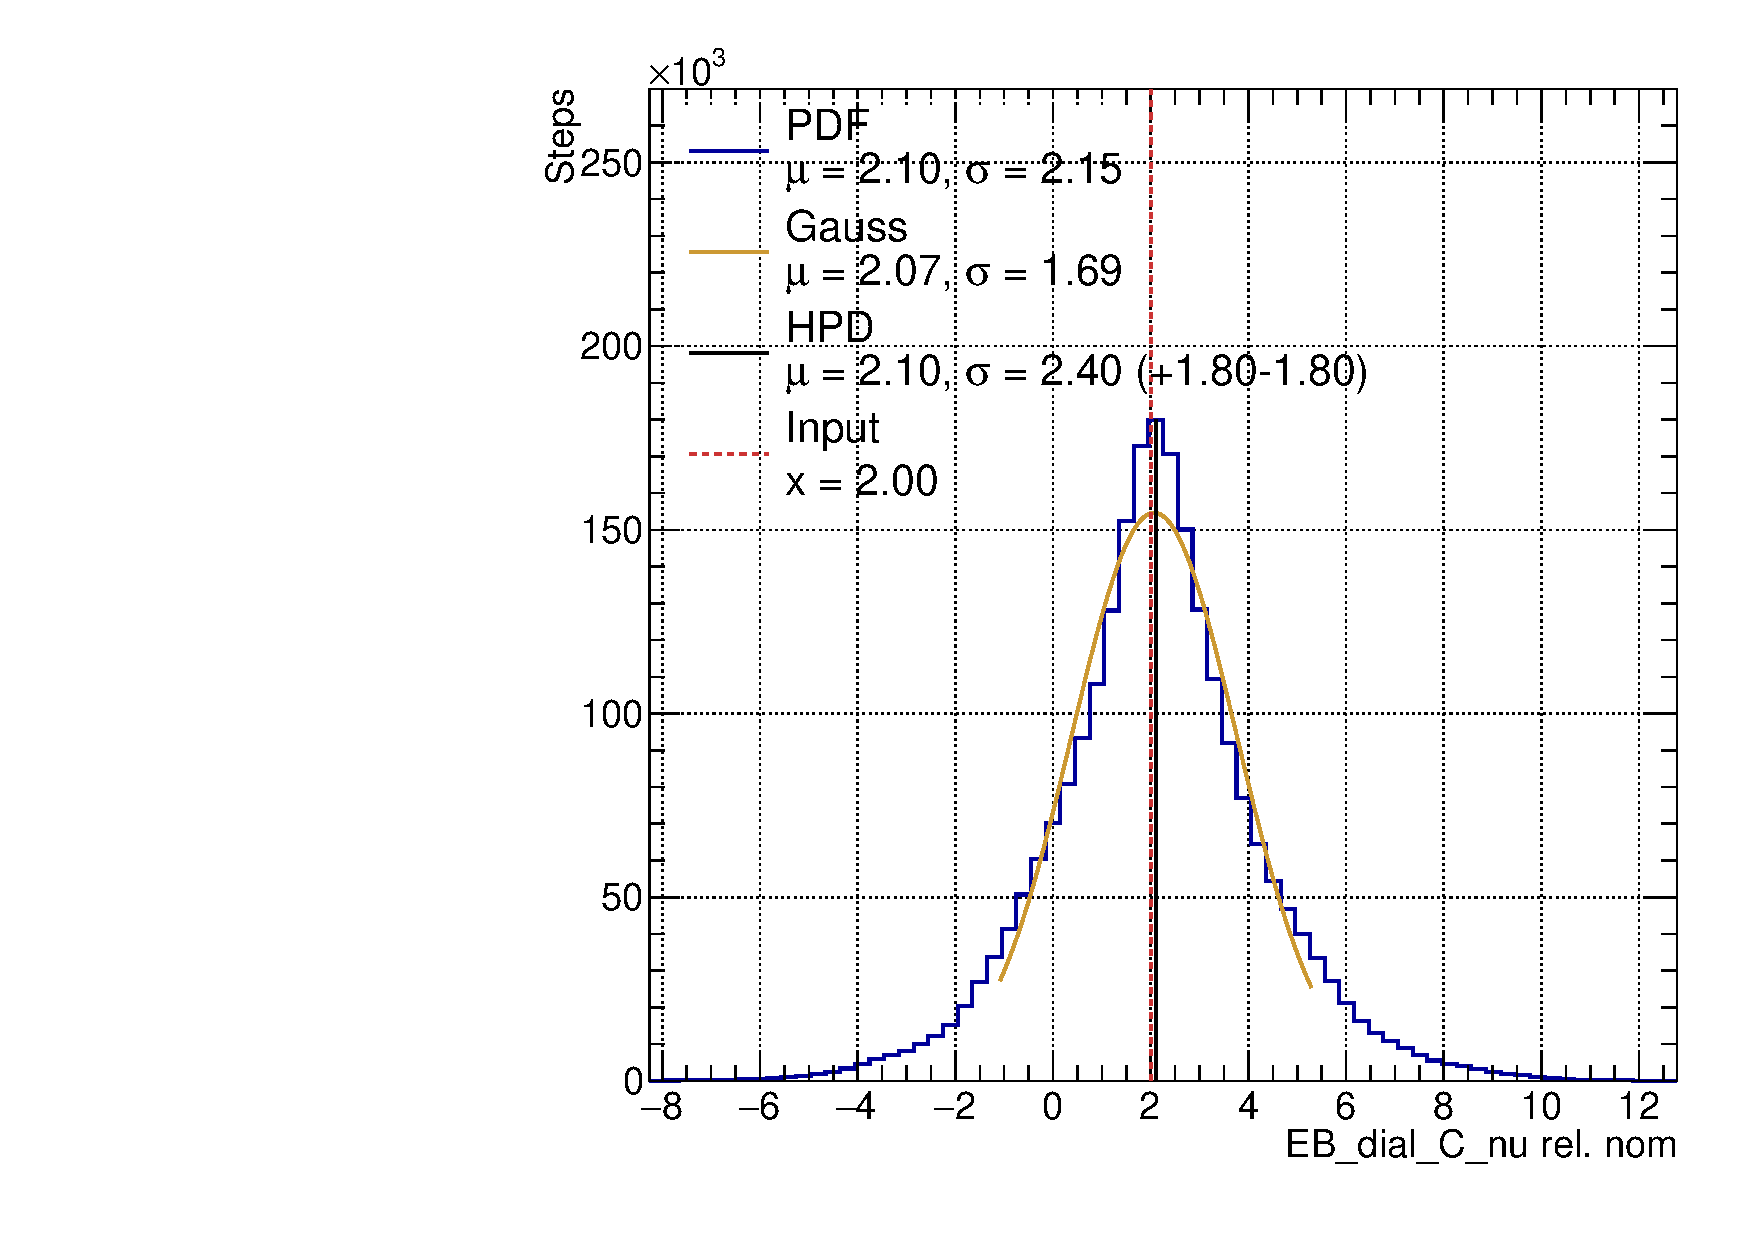
\includegraphics[width=0.73\linewidth]{figs/EB_dial_C_nuAsmv}
  \caption{$E_{b}\nu$ C}
\end{subfigure}
\begin{subfigure}{.48\textwidth}
  \centering
  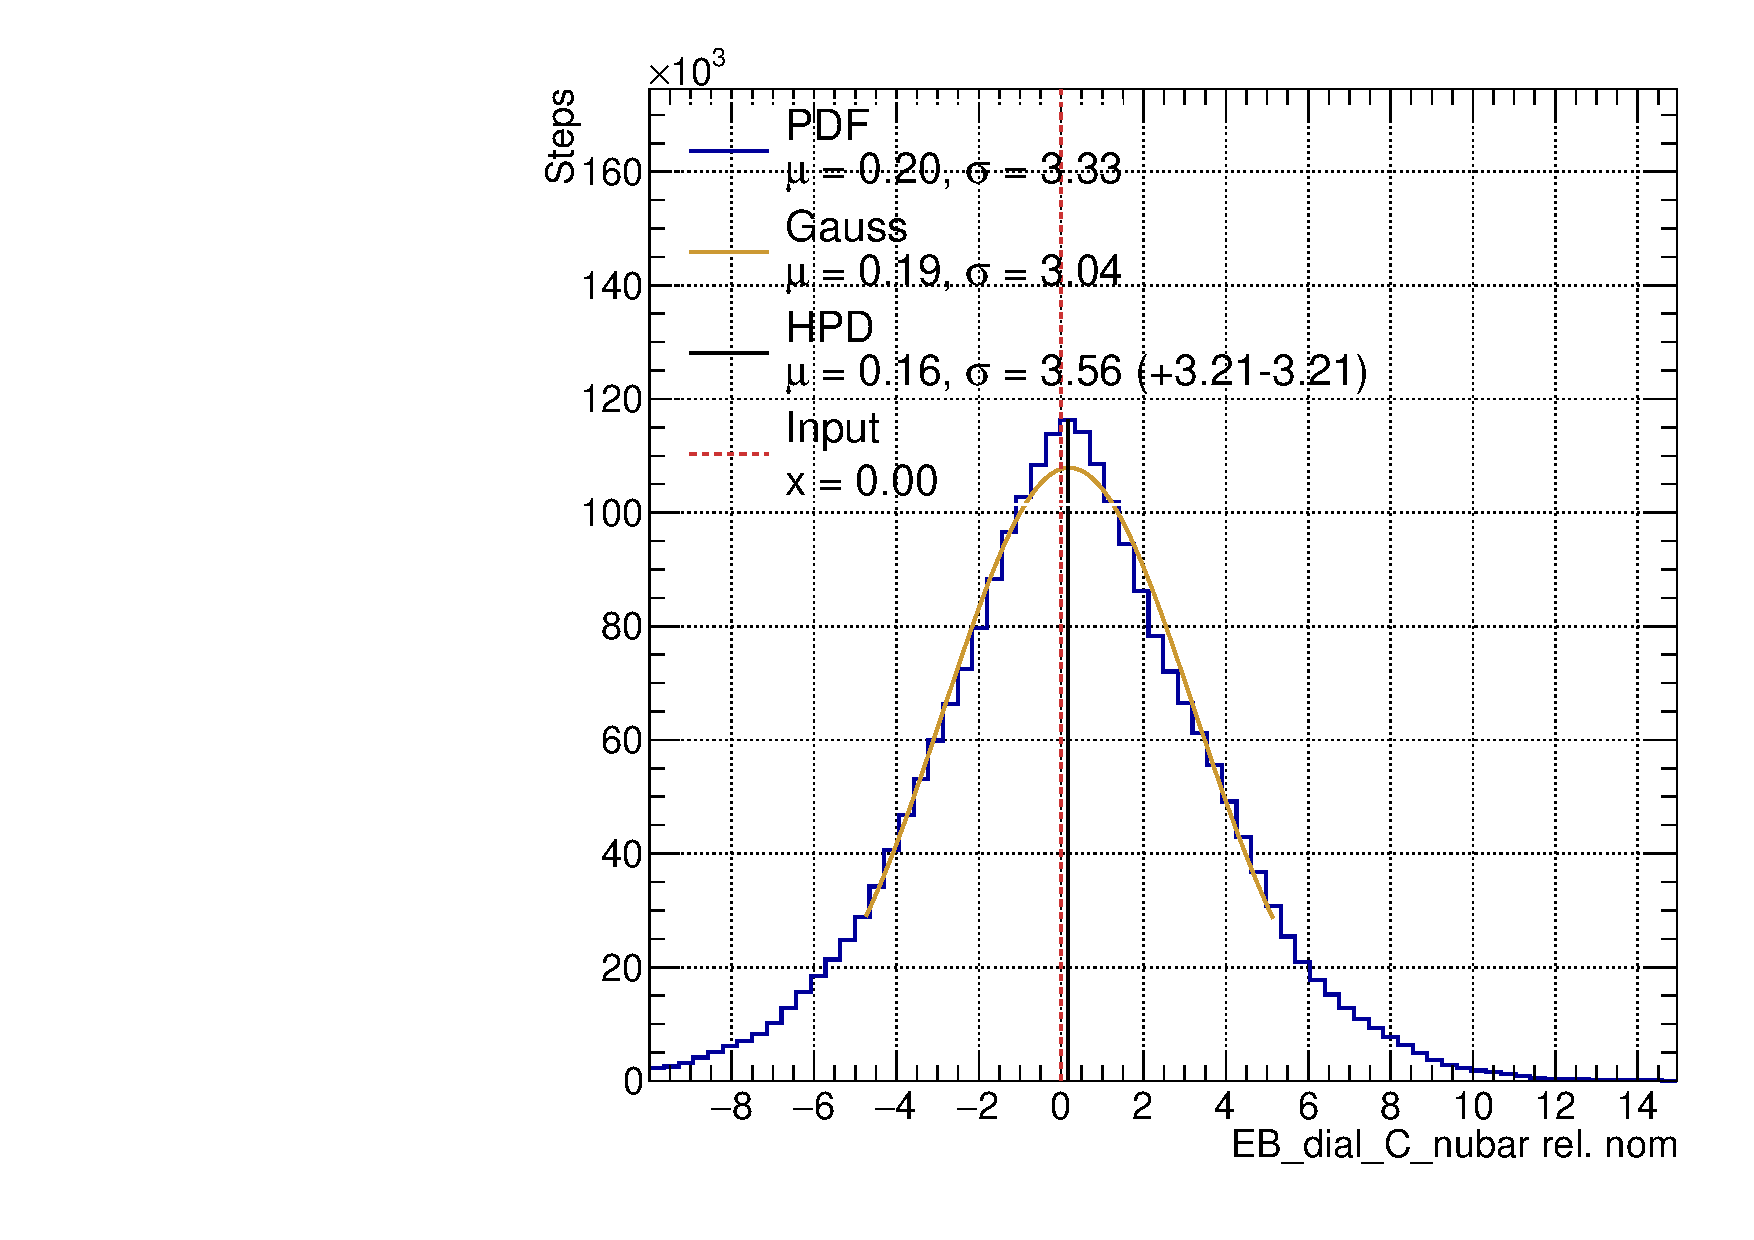
\includegraphics[width=0.73\linewidth]{figs/EB_dial_C_nubarAsmv}
  \caption{$E_{b}\bar{\nu}$ C}
\end{subfigure} \\
\begin{subfigure}{.48\textwidth}
  \centering
  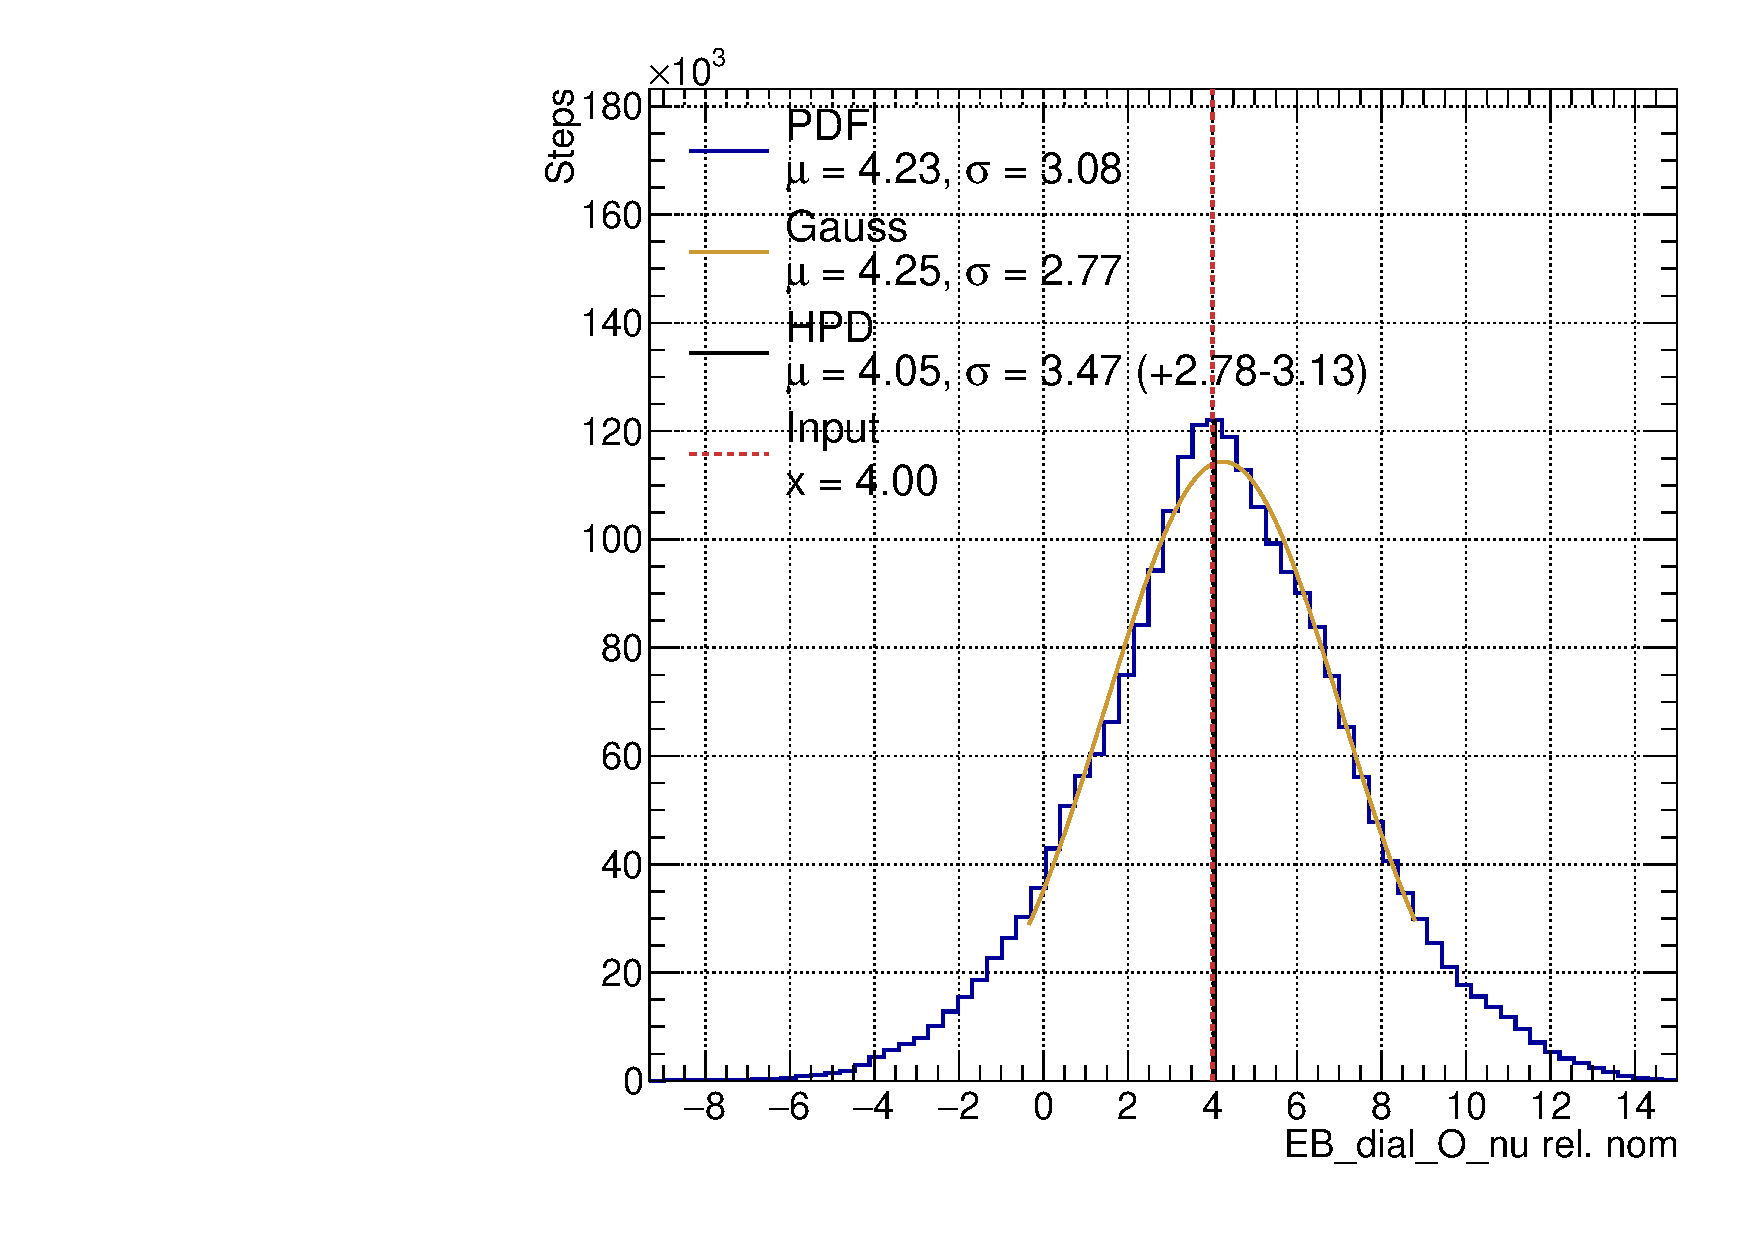
\includegraphics[width=0.73\linewidth]{figs/EB_dial_O_nuAsmv}
  \caption{$E_{b}\nu$ O}
\end{subfigure}
\begin{subfigure}{.48\textwidth}
  \centering
  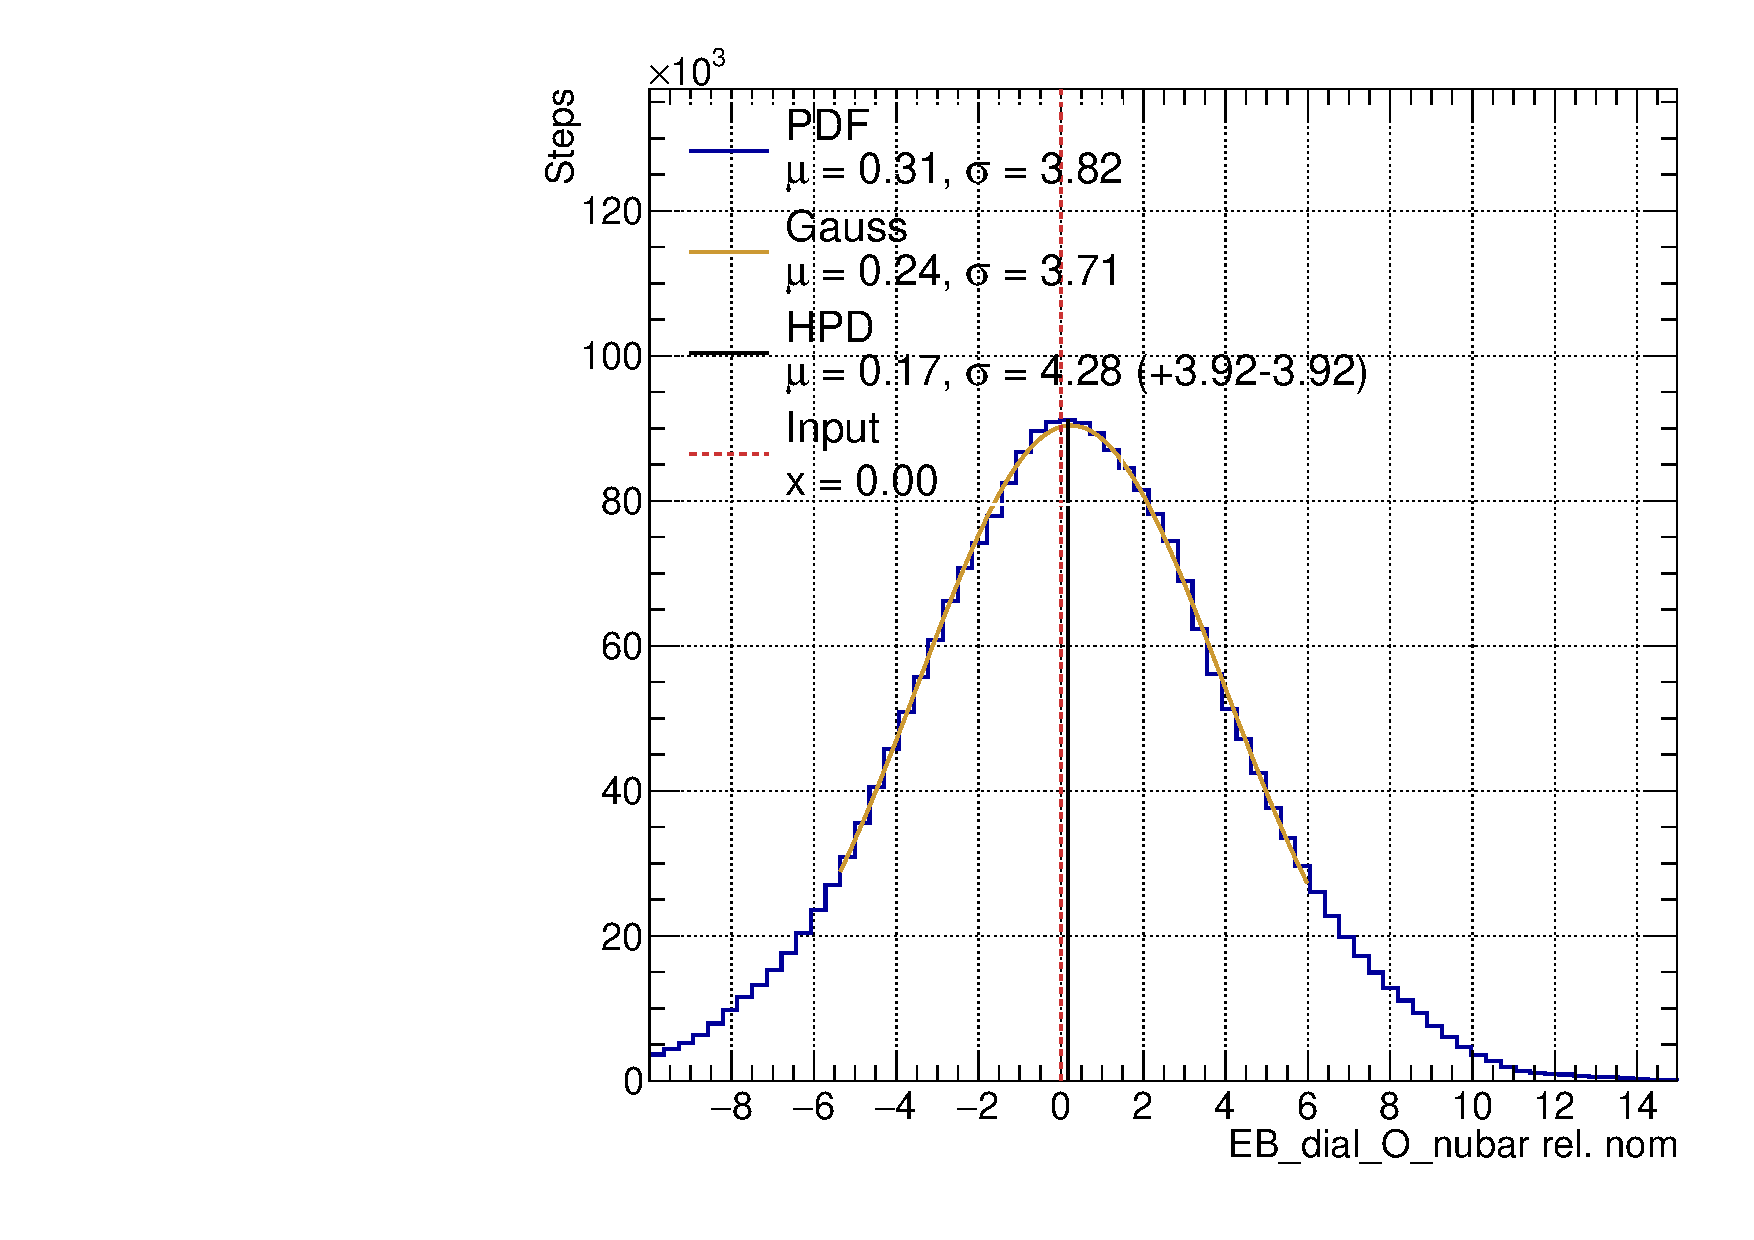
\includegraphics[width=0.73\linewidth]{figs/EB_dial_O_nubarAsmv}
  \caption{$E_{b}\bar{\nu}$ O}
\end{subfigure}
\caption{Posterior distributions for the binding energy parameters from an Asimov fit.}
\label{fig:Ebasimov}
\end{figure}

However, for fits to data the posteriors contain many discontinuities as shown in Figure \ref{fig:Ebdata}. This is not seen for other parameters. When reweighting, either by spline or normalisation, the change in the log-likelihood is continuous. As the parameter varies, the change in the penalty contribution, and the change in the number of events in each bin, and therefore the sample contribution, are both smooth. However, for this direct shift in lepton momentum, the sample contribution to the likelihood only changes if an event crosses a bin boundary. There are therefore threshold values of each parameter where several events cross boundaries and cause discontinuous changes in the log-likelihood.

\begin{figure}[t]
\centering
\begin{subfigure}{.48\textwidth}
  \centering
  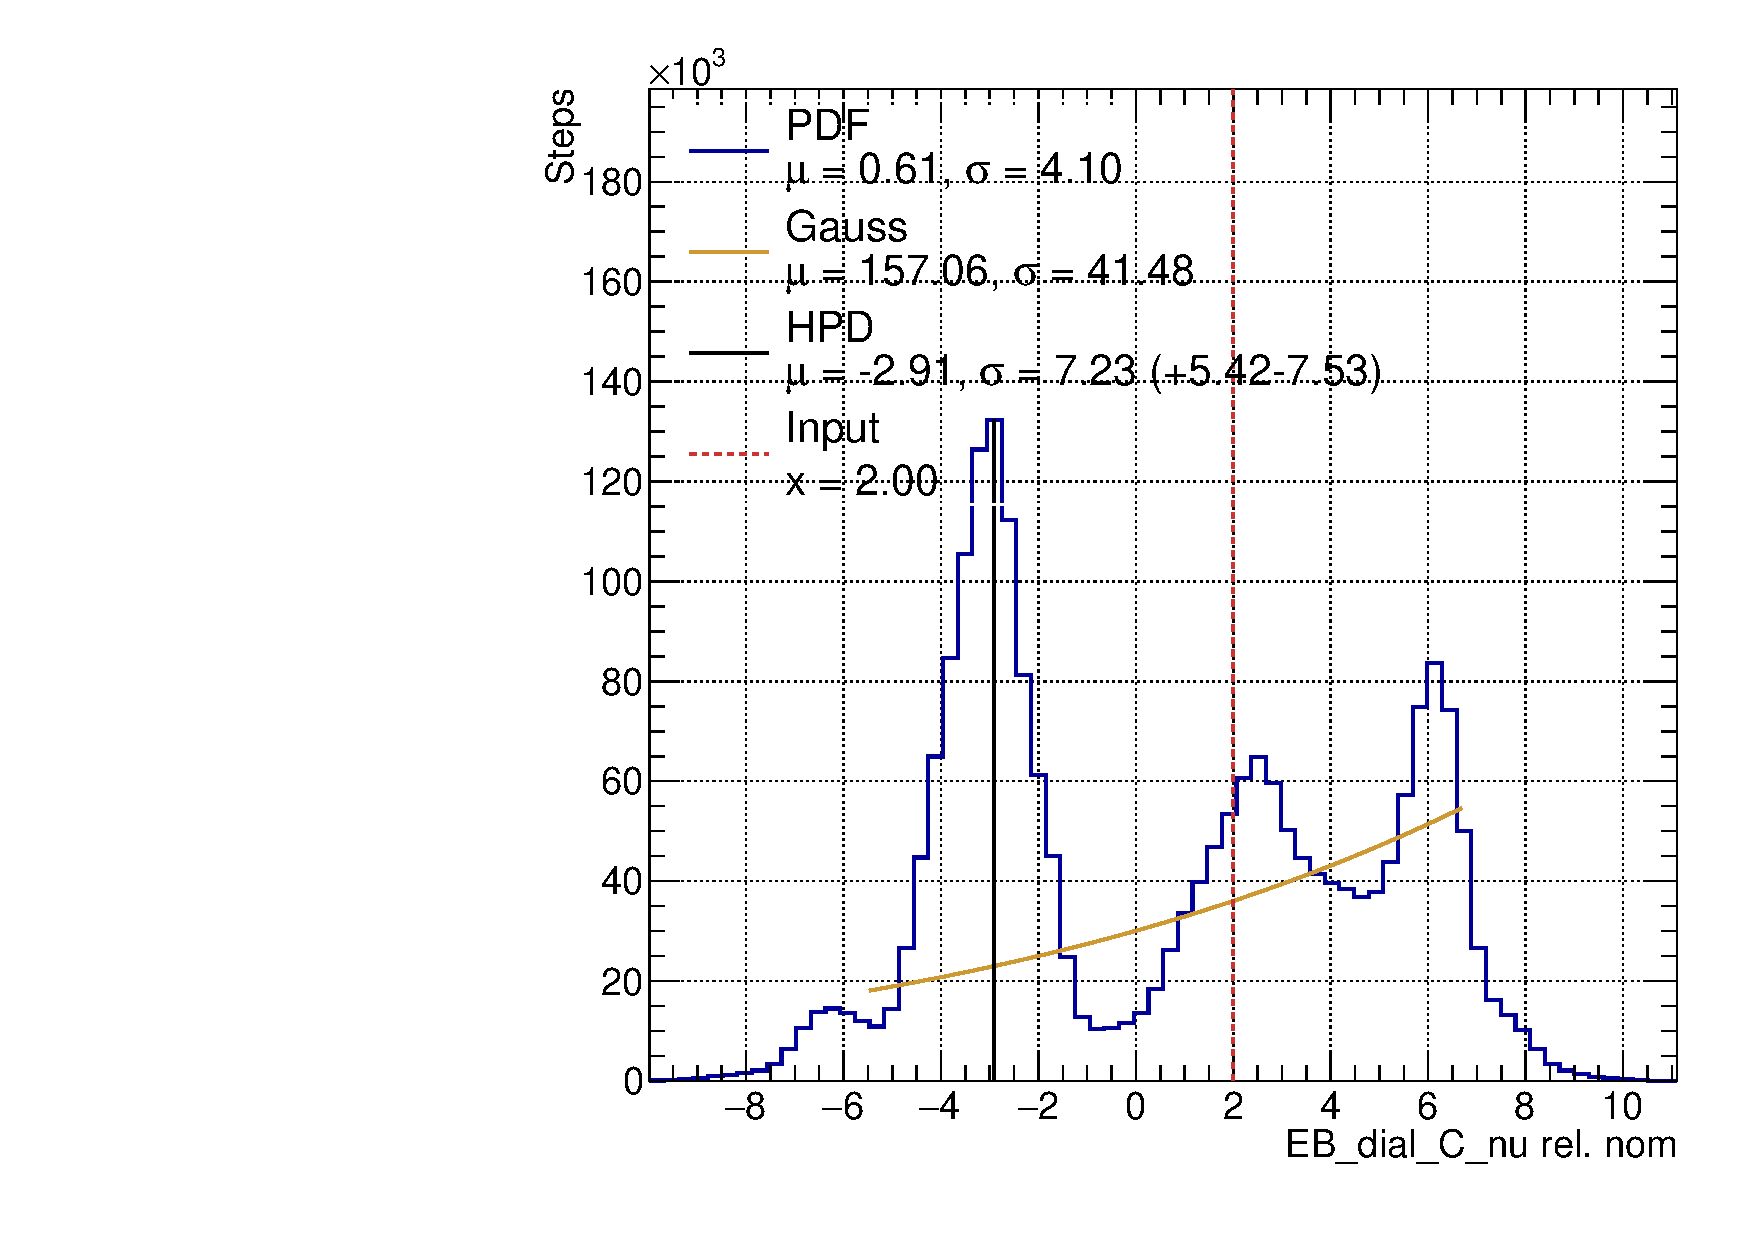
\includegraphics[width=0.73\linewidth]{figs/EB_dial_C_nuData}
  \caption{$E_{b}\nu$ C}
\end{subfigure}
\begin{subfigure}{.48\textwidth}
  \centering
  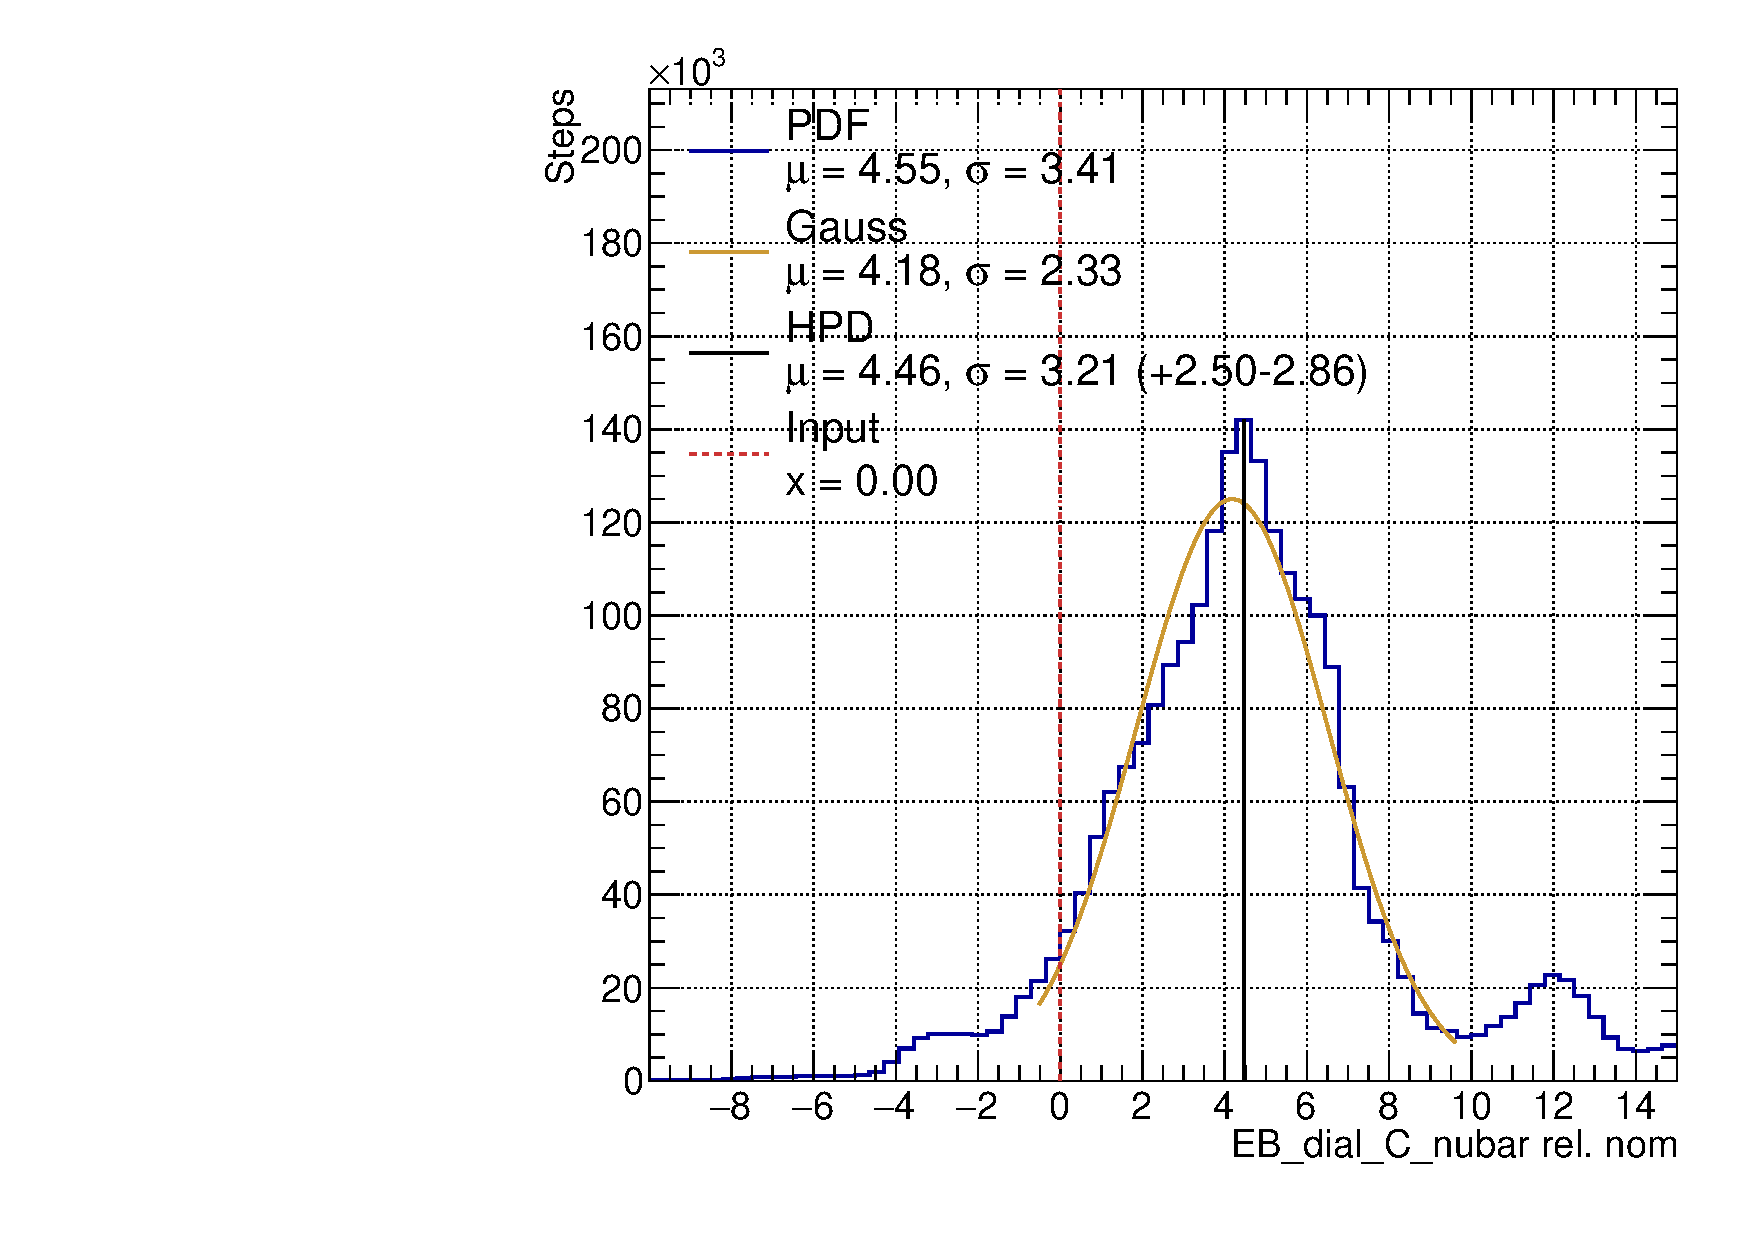
\includegraphics[width=0.73\linewidth]{figs/EB_dial_C_nubarData}
  \caption{$E_{b}\bar{\nu}$ C}
\end{subfigure} \\
\begin{subfigure}{.48\textwidth}
  \centering
  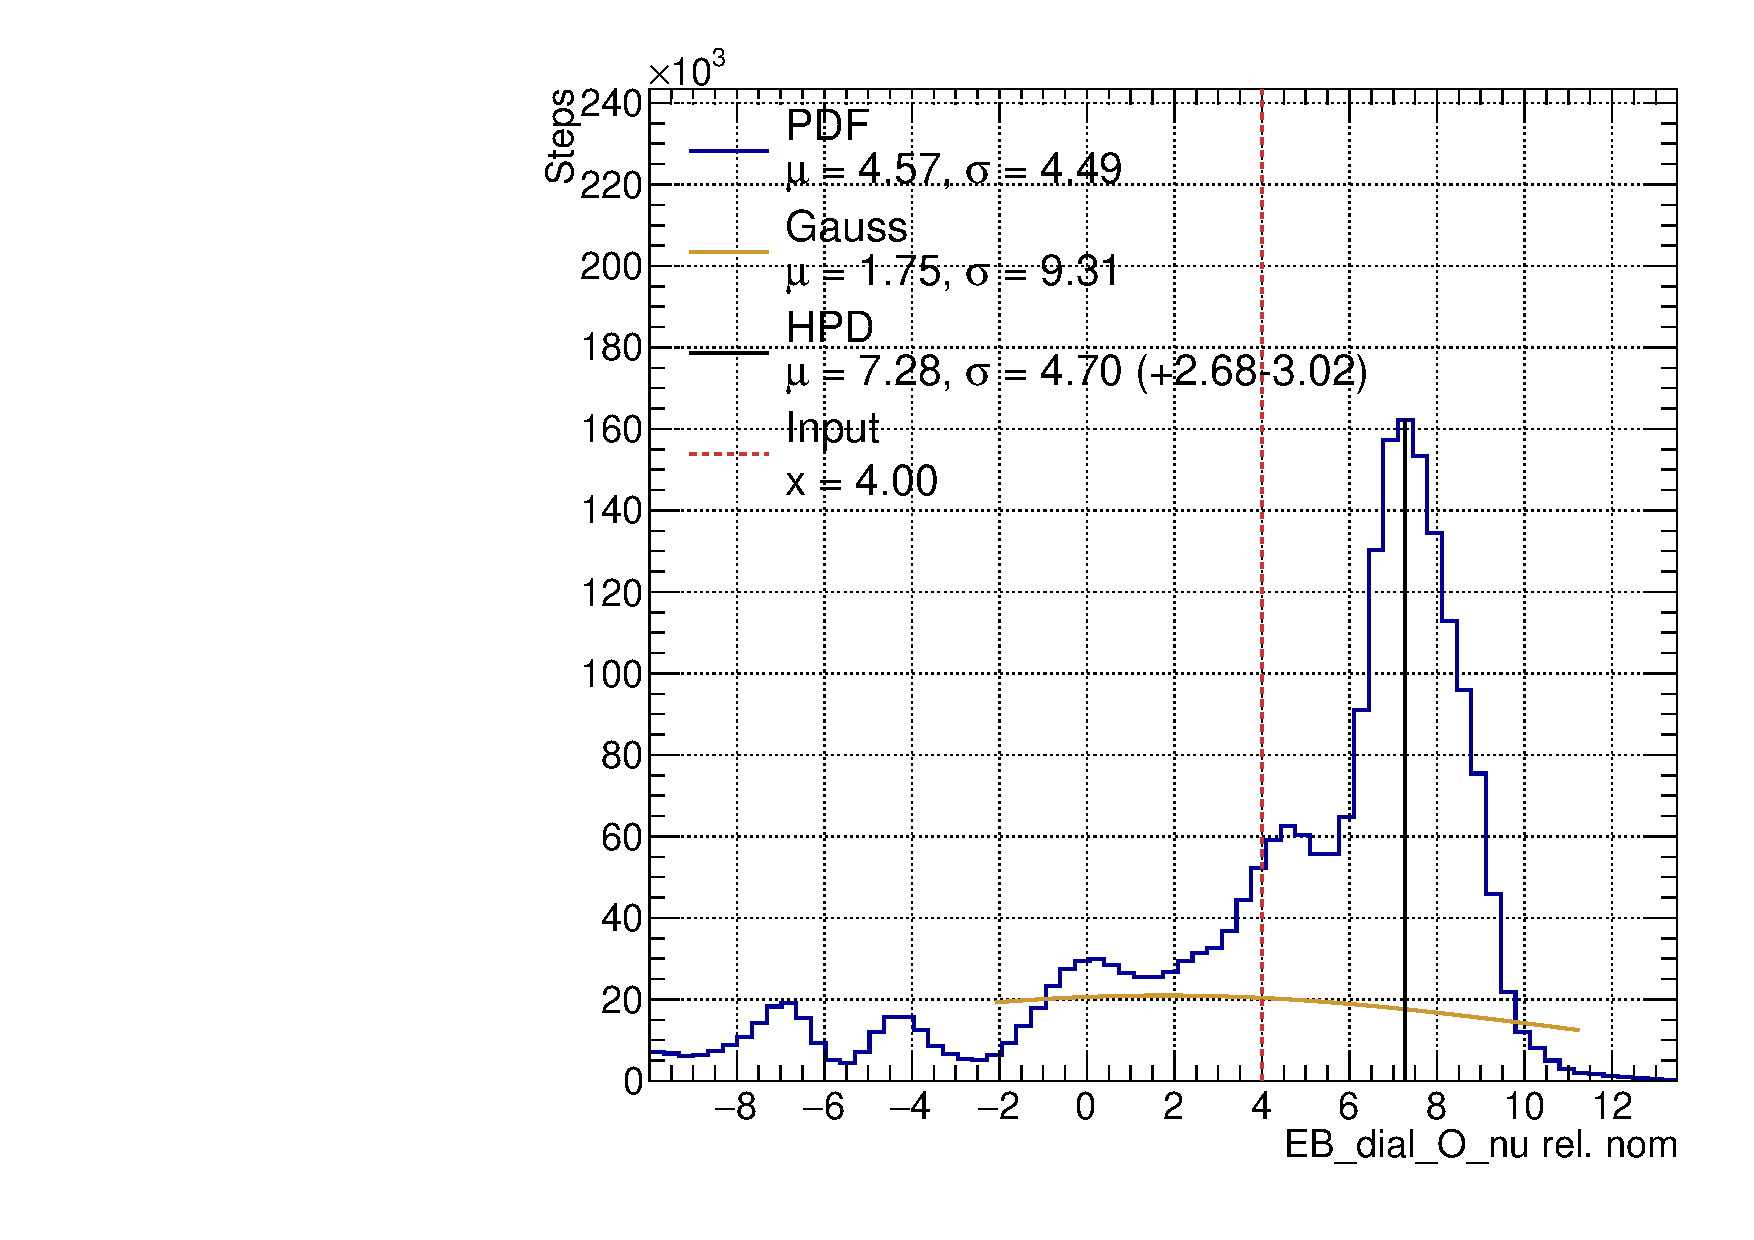
\includegraphics[width=0.73\linewidth]{figs/EB_dial_O_nuData}
  \caption{$E_{b}\nu$ O}
\end{subfigure}
\begin{subfigure}{.48\textwidth}
  \centering
  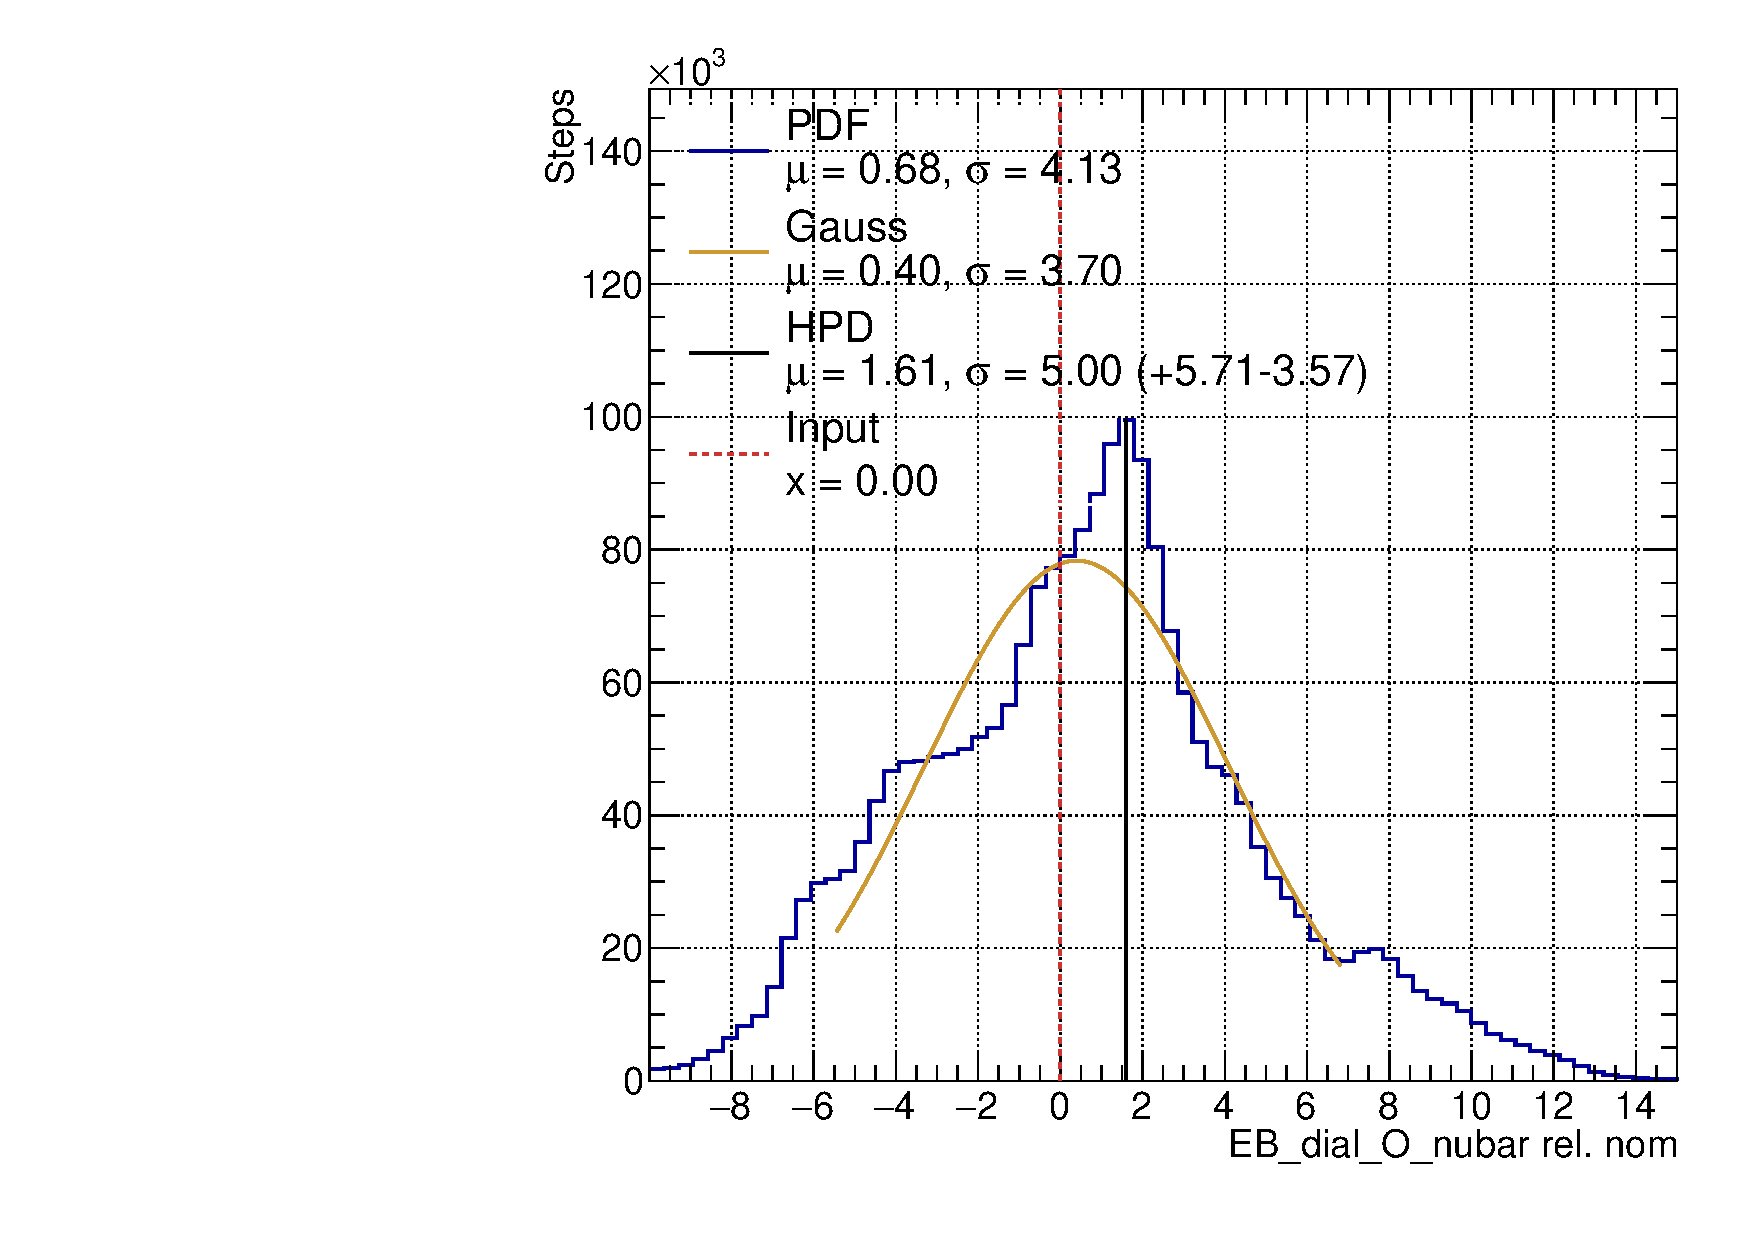
\includegraphics[width=0.73\linewidth]{figs/EB_dial_O_nubarData}
  \caption{$E_{b}\bar{\nu}$ O}
\end{subfigure}
\caption{Posterior distributions for the binding energy parameters from a data fit.}
\label{fig:Ebdata}
\end{figure}

To show this is what causes the discontinuities, a fluctuated version of the nominal MC was produced. This was done by setting the number of events in each bin to be a random number from a Poisson distribution, with a mean equal to the nominal bin content. This ensured the number of events in each bin was an integer. The fluctuated MC was fitted to the nominal MC, and the posterior distributions for the $E_b$ parameters are shown in Figure \ref{fig:Ebfluc}. The fact that these are non-Gaussian and discontinuous, despite them being continuous and Gaussian in the regular Asimov fit, shows that the effect is caused by the discrete shifts to integer events.

Furthermore, Figure \ref{fig:Ebfluc} also shows the $E_b$ distributions for a fluctuated Asimov fit using the non-rectangular binning described in Section \ref{sec:nonrecbinning}. The peaks in the distributions, caused by the shifting of discrete events across bin boundaries, move positions between the two fits. This shows the location of the peaks in $E_{b}$ is very dependent on the binning. This is much more of a significant effect for $E_b$, as the parametrisation directly shifts events rather than reweighting them. Changes in the likelihood therefore only occur when the events cross bin boundaries, and so the parameter is sensitive to where those boundaries are. Different binnings can therefore produce different fit results.

\begin{figure}
\centering
\begin{subfigure}{.48\textwidth}
  \centering
  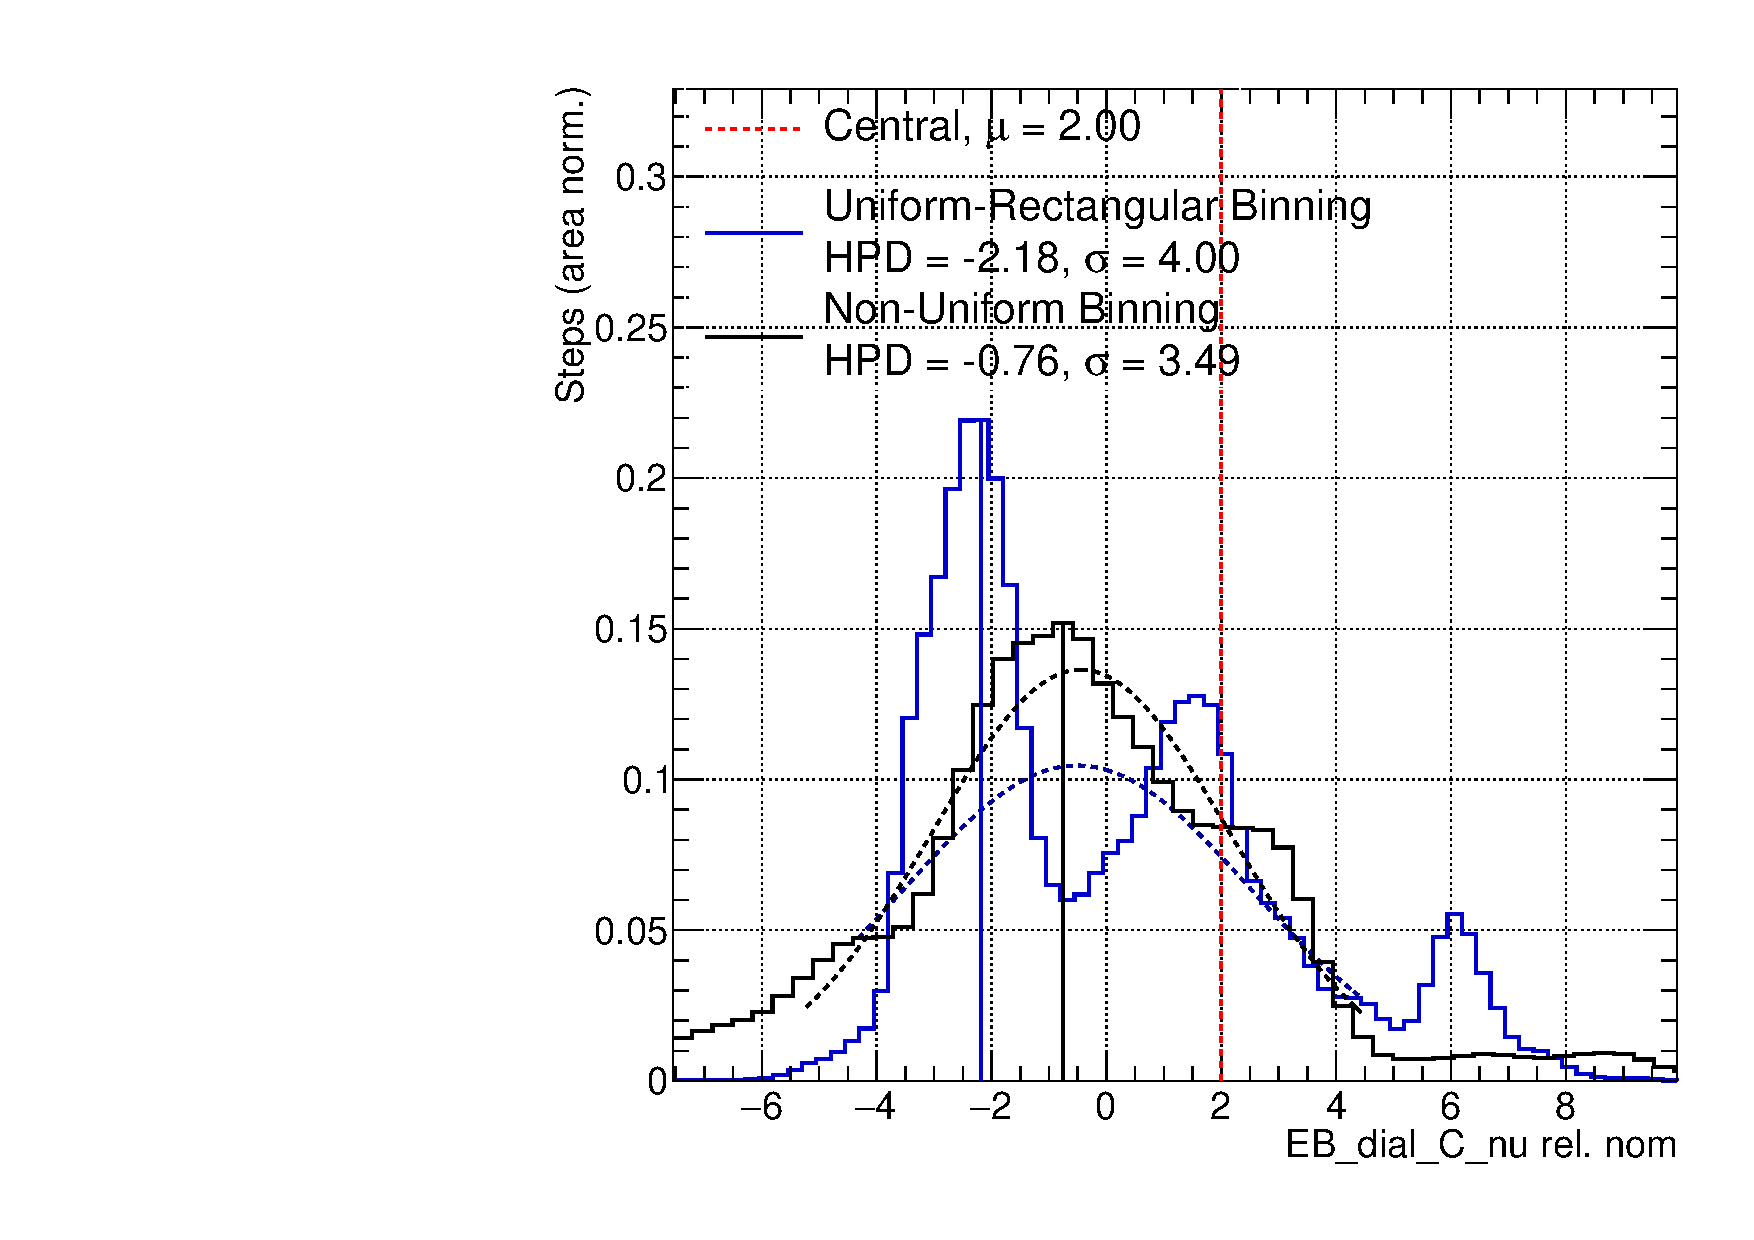
\includegraphics[width=0.73\linewidth]{figs/EB_dial_C_nuFluc2}
  \caption{$E_{b}\nu$ C}
\end{subfigure}
\begin{subfigure}{.48\textwidth}
  \centering
  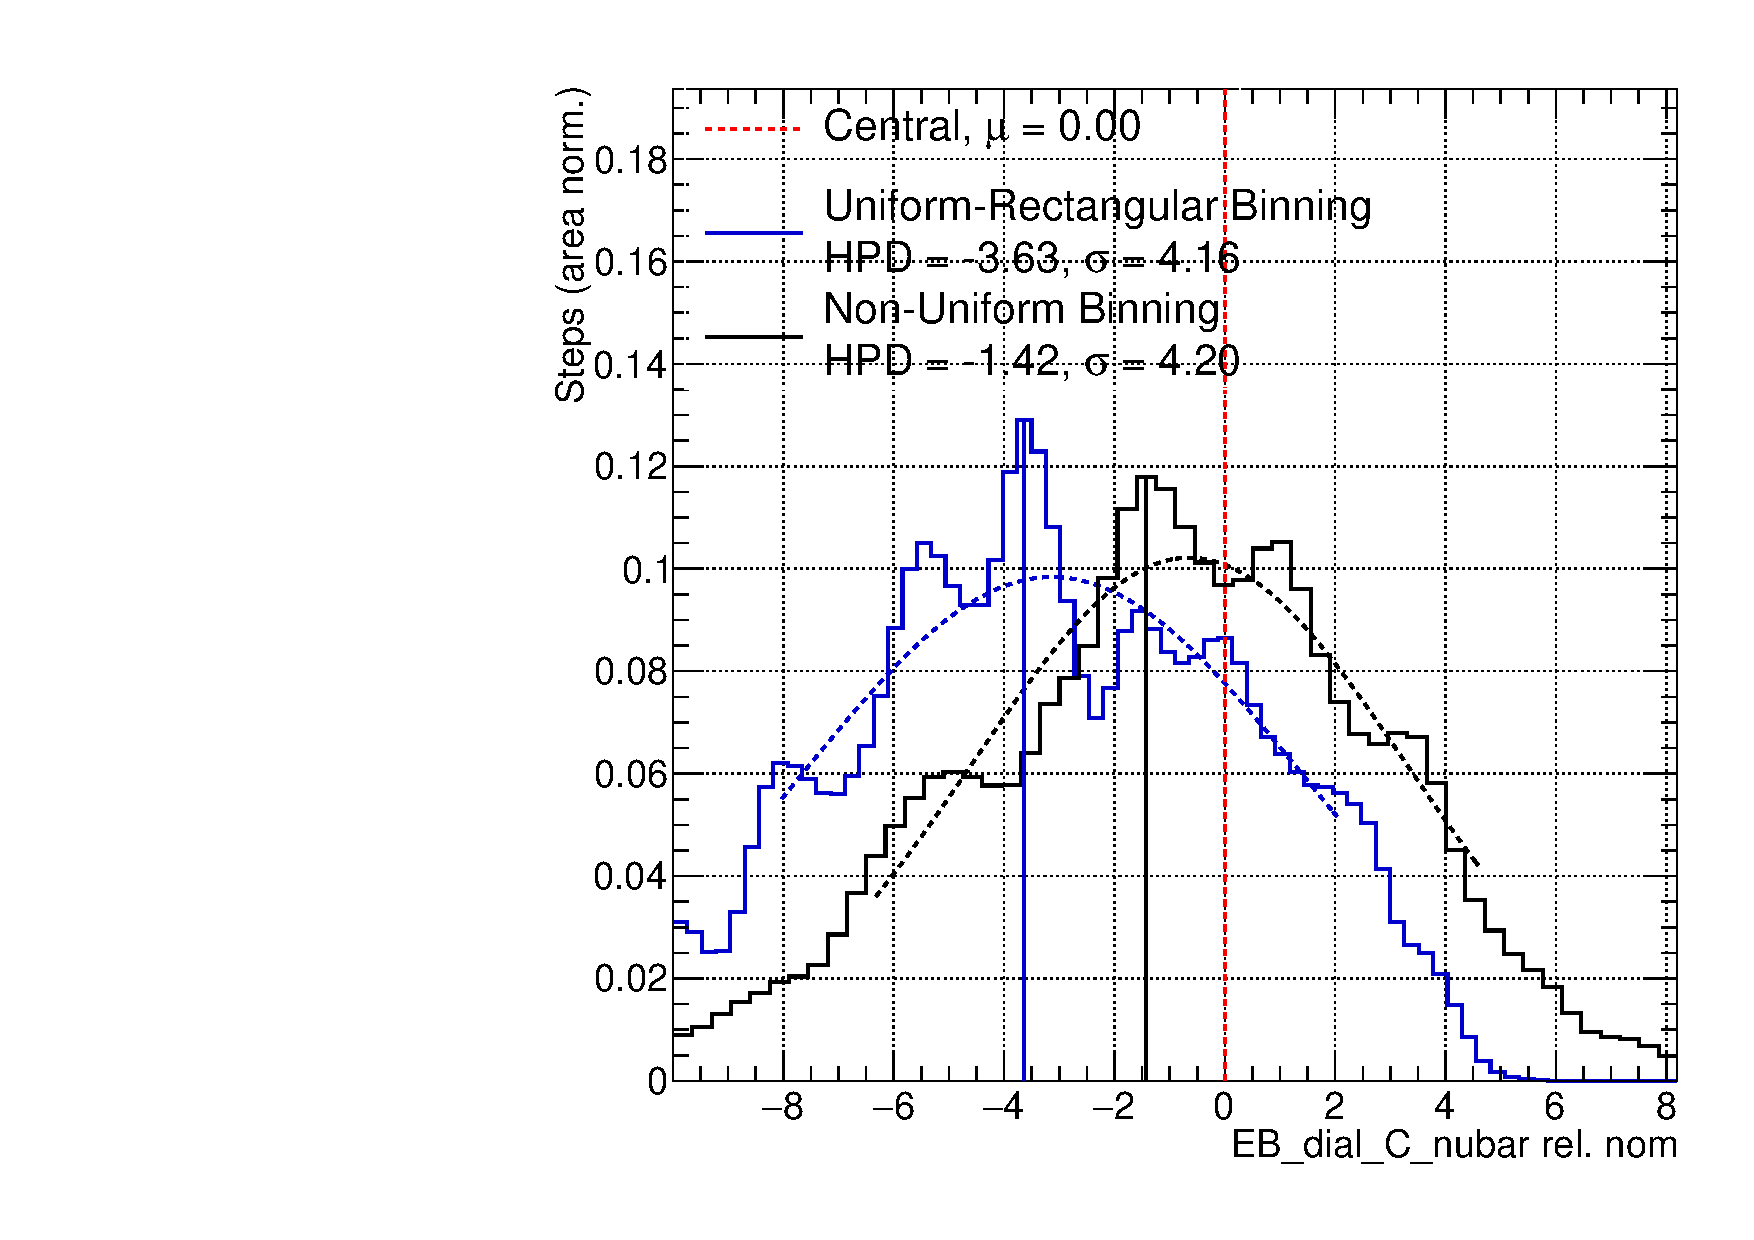
\includegraphics[width=0.73\linewidth]{figs/EB_dial_C_nubarFluc2}
  \caption{$E_{b}\bar{\nu}$ C}
\end{subfigure} \\
\begin{subfigure}{.48\textwidth}
  \centering
  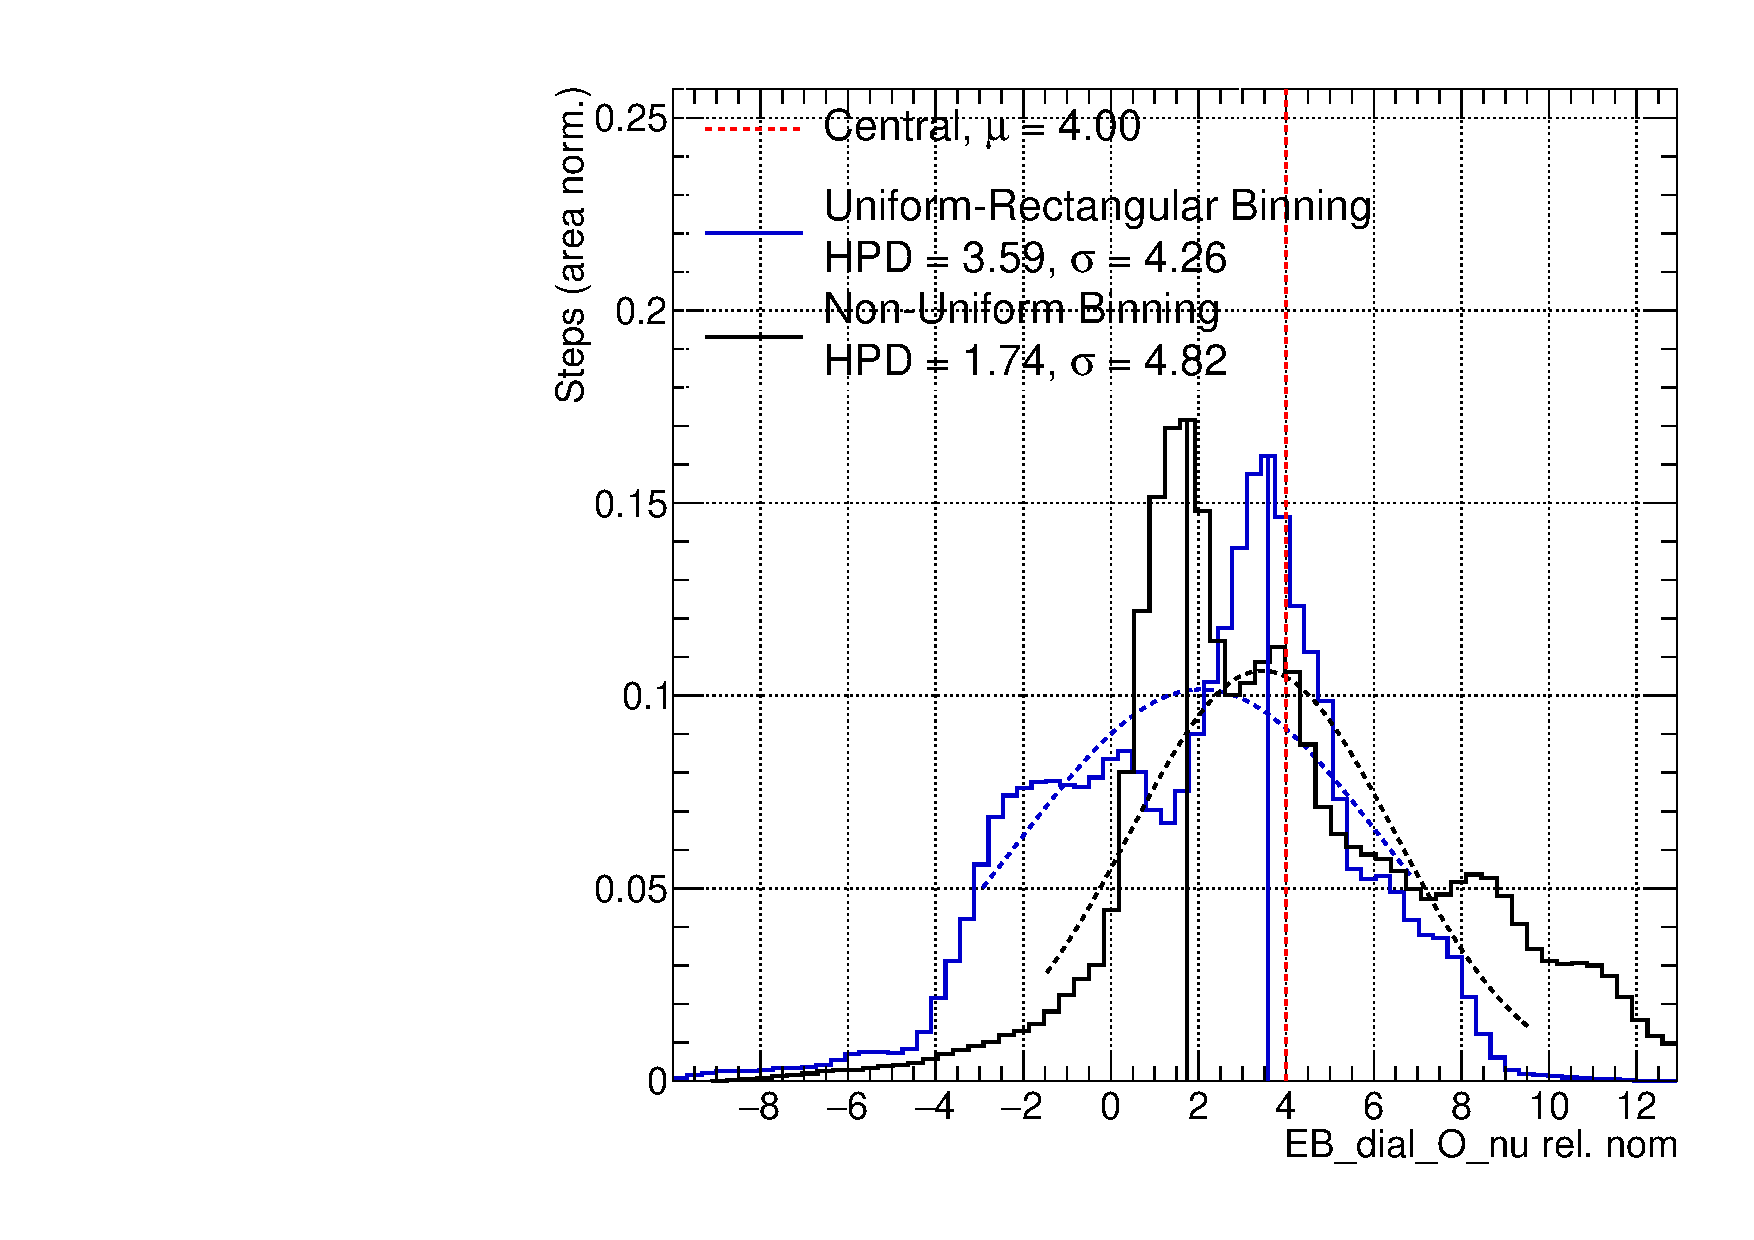
\includegraphics[width=0.73\linewidth]{figs/EB_dial_O_nuFluc2}
  \caption{$E_{b}\nu$ O}
\end{subfigure}
\begin{subfigure}{.48\textwidth}
  \centering
  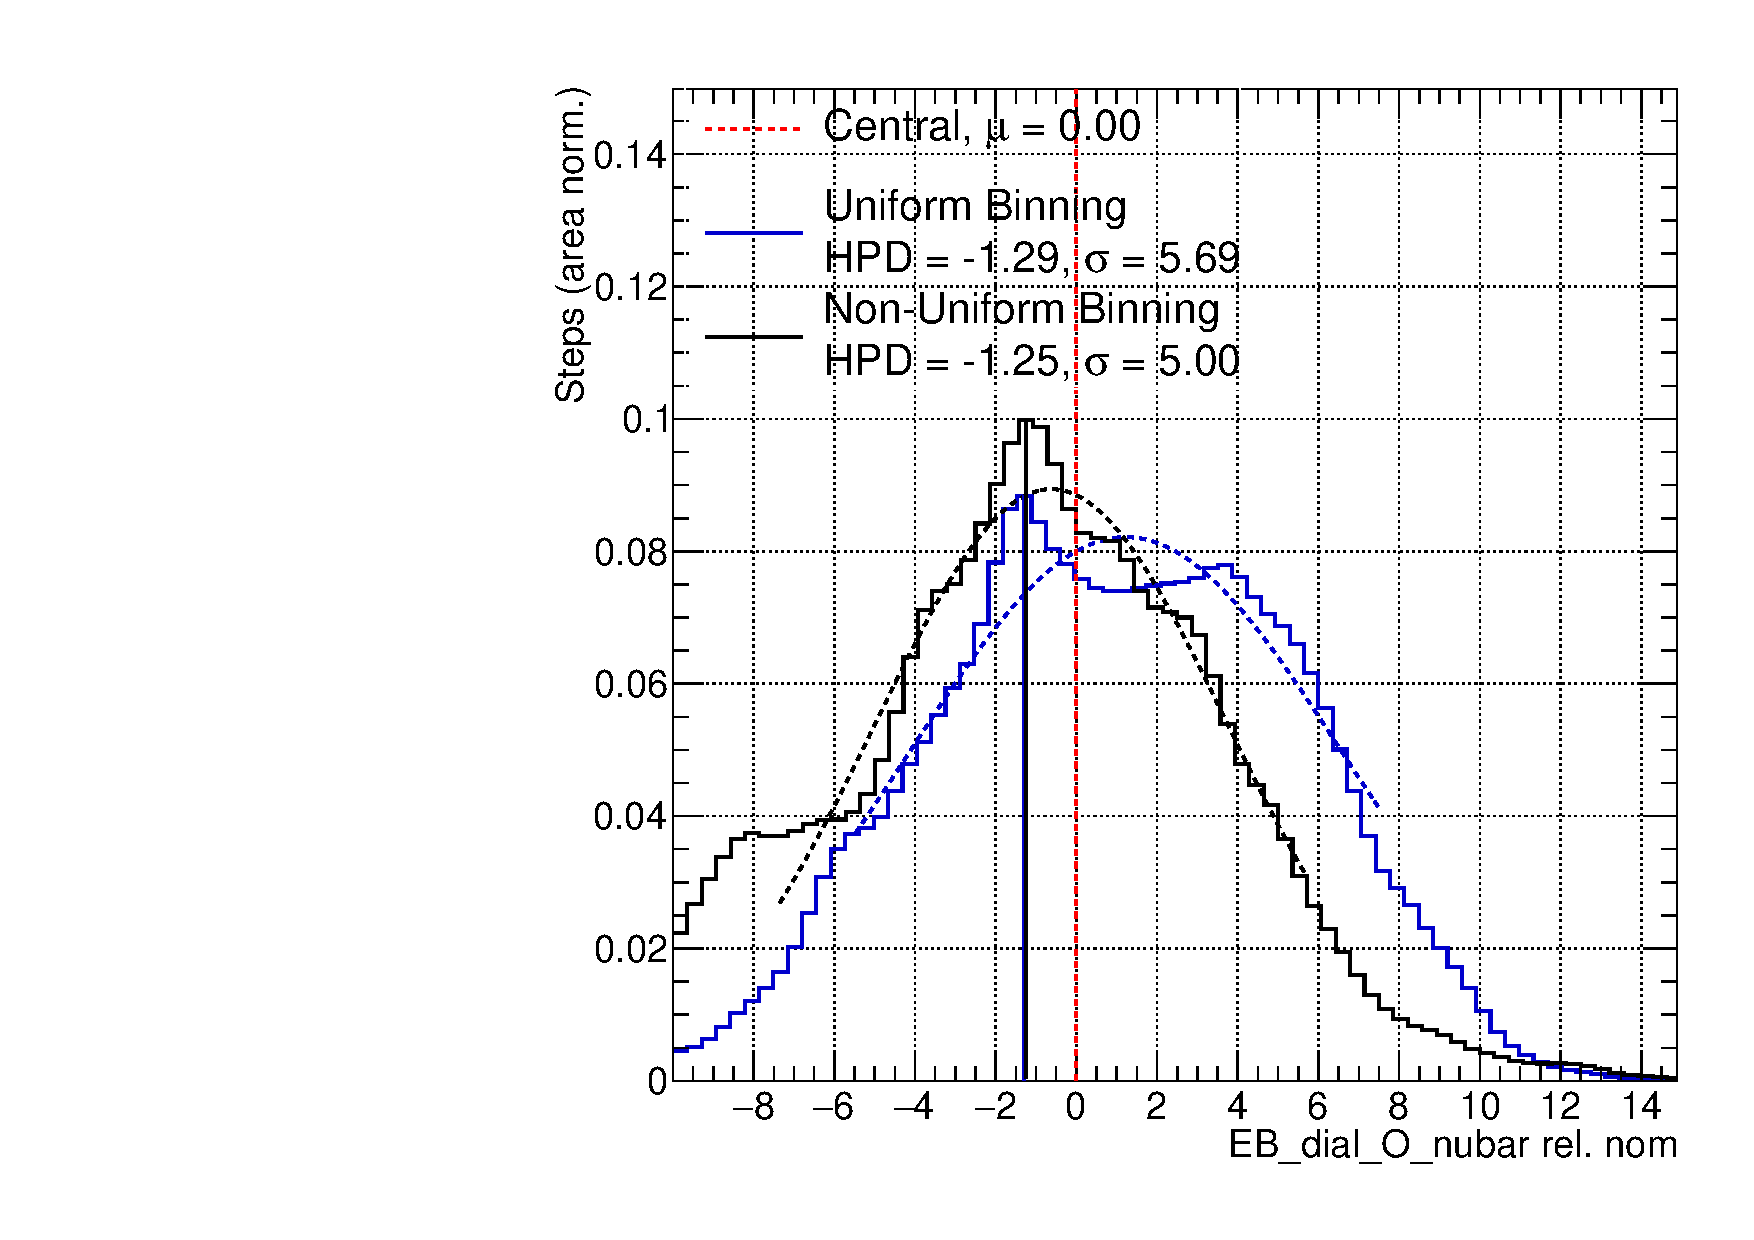
\includegraphics[width=0.73\linewidth]{figs/EB_dial_O_nubarFluc2}
  \caption{$E_{b}\bar{\nu}$ O}
\end{subfigure}
\caption{Posterior distributions for the binding energy parameters from fits to fluctuated Asimov data using uniform and non-uniform rectangular fit binnings.}
\label{fig:Ebfluc}
\end{figure}

As the BANFF fit uses a gradient descent, the discontinuities in the binding energy parameter likelihoods can prevent the fit from converging. To avoid this, rather than directly shift the outgoing lepton momentum of events the BANFF use an effective reweighting. This aims to smoothly replicate the shifting of events by increasing and decreasing the events in a continuous manner. Template distributions were produced for each sample for a number of knot points for each parameter. Bin-by-bin splines were then produced by interpolating between the number of events in each bin at different knot values. This process is described in more detail in \cite{tn395}. 

Figure \ref{fig:EbLLHBANFF} shows log-likelihood scans for the binding energy parameters in both the MaCh3 and BANFF frameworks. For the BANFF fit, these are smoother, but they closely trace the MaCh3 distributions. This is the intended behaviour of the splines: to smooth over discontinuities while retaining the overall shape. However, the fact that there is not perfect agreement shows that the spline process cannot completely represent the direct momentum shifts. The implementation of the binding energy uncertainty used in MaCh3 is therefore a more accurate method.

\begin{figure}
\centering
\begin{subfigure}{.48\textwidth}
  \centering
  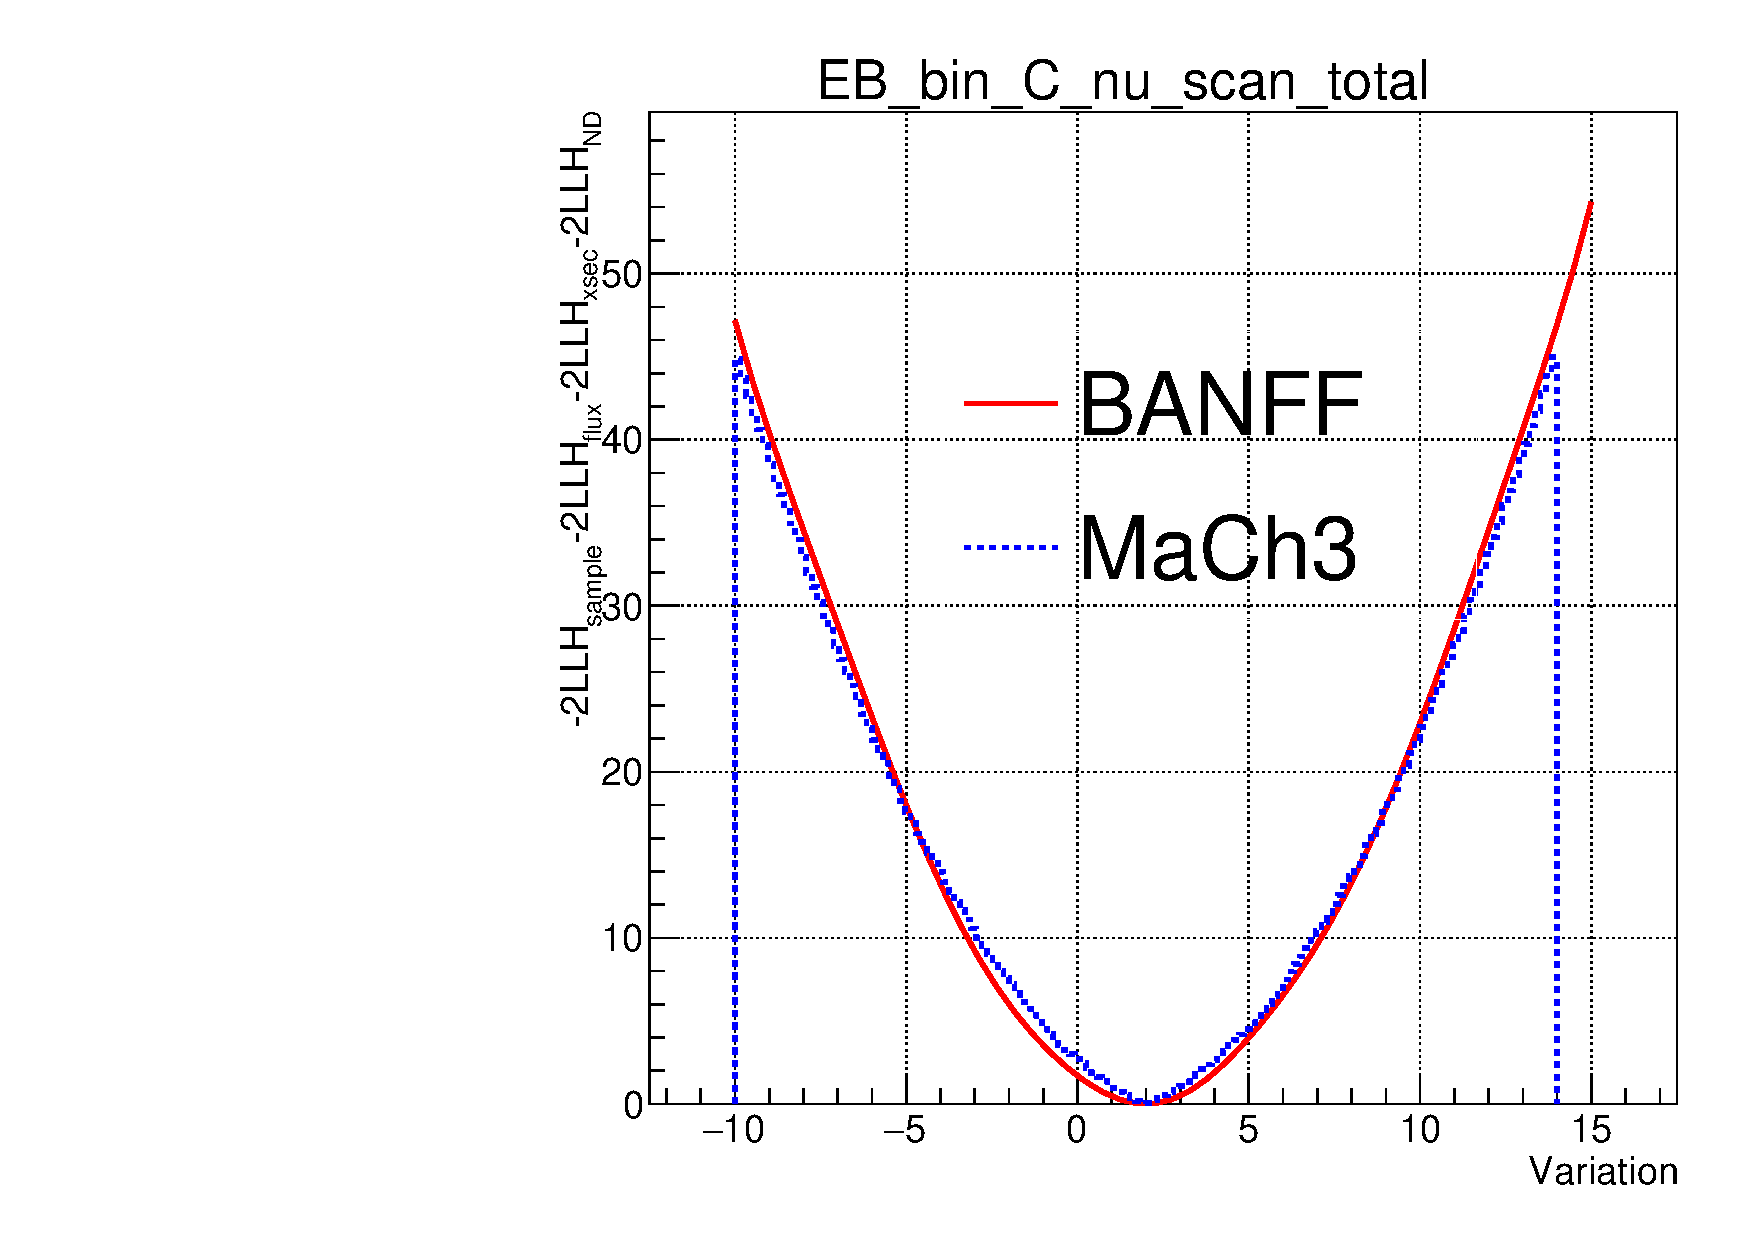
\includegraphics[width=0.73\linewidth]{figs/EB_dial_C_nu_full_FullLLH}
  \caption{$E_{b}\nu$ C}
\end{subfigure}
\begin{subfigure}{.48\textwidth}
  \centering
  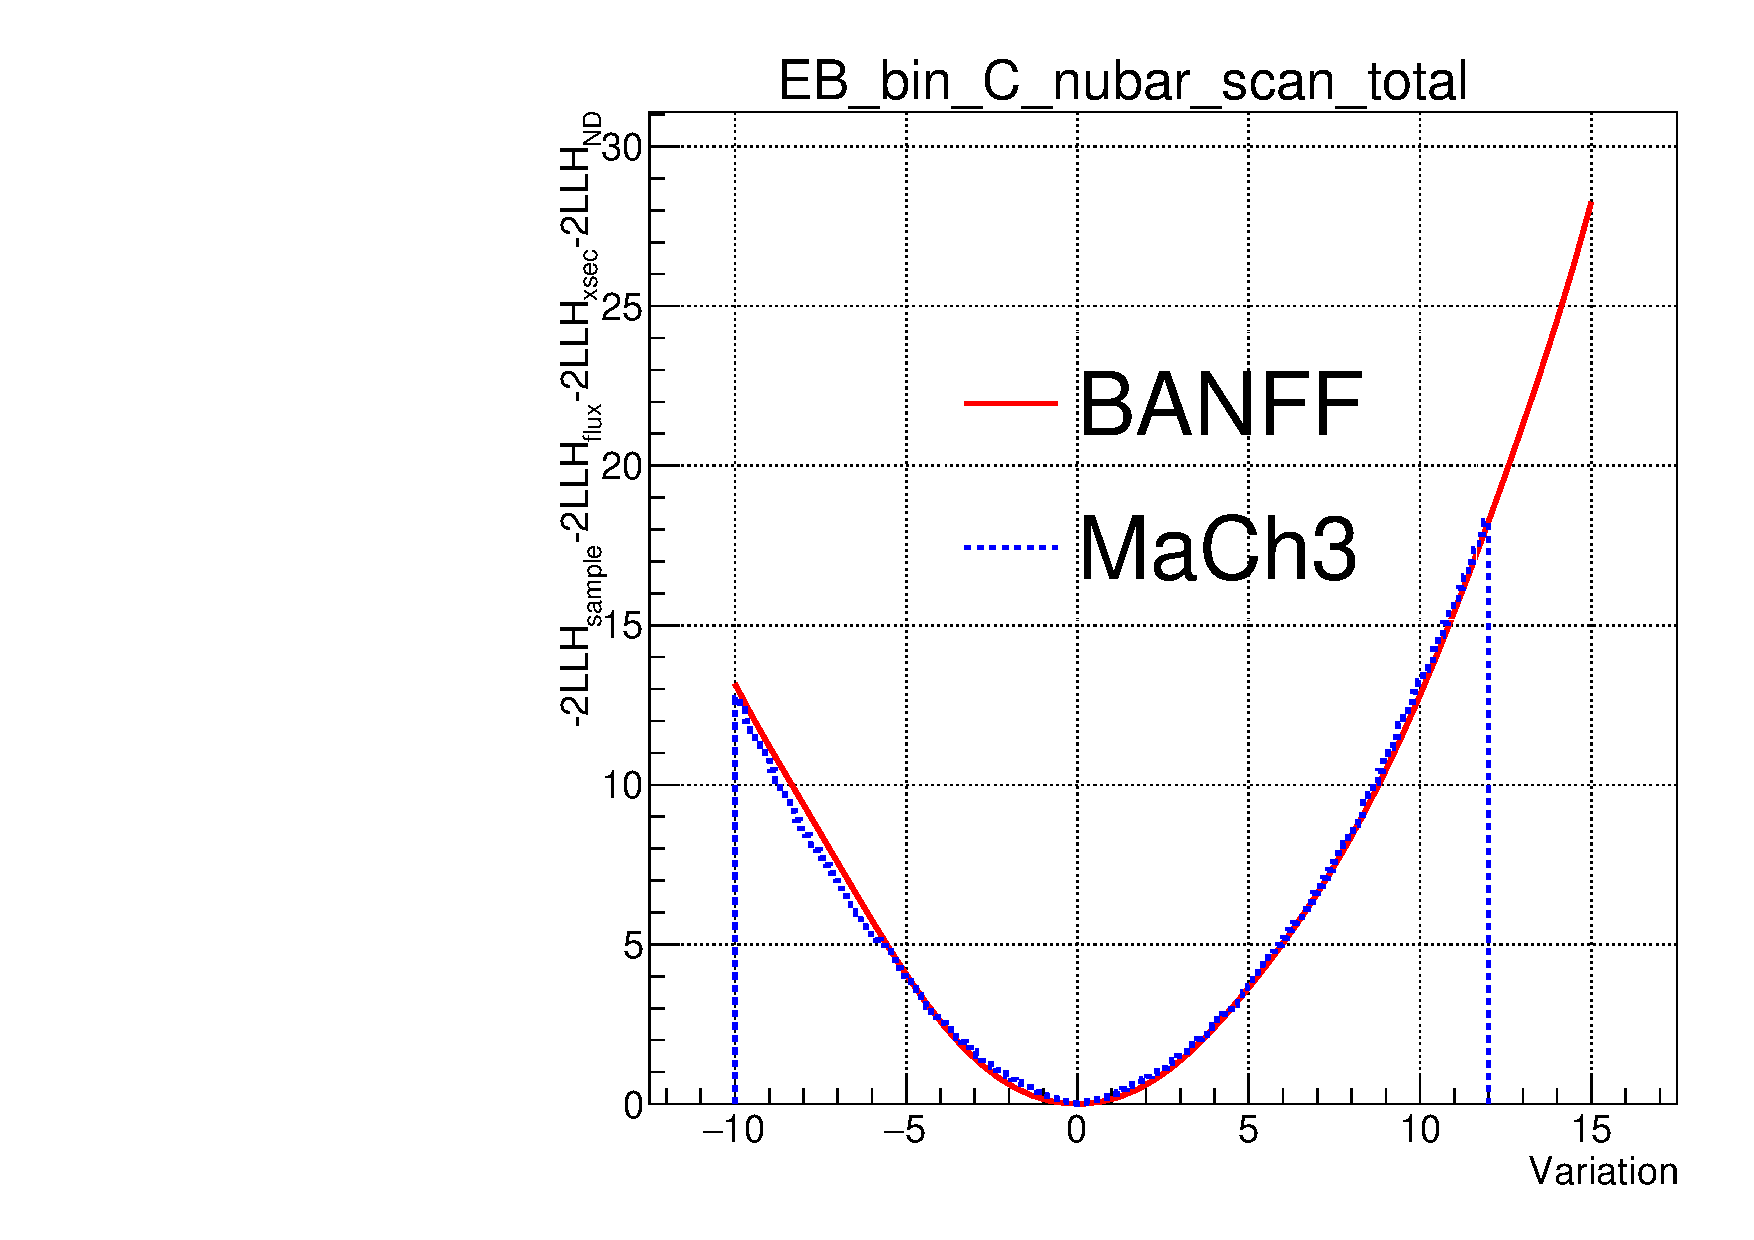
\includegraphics[width=0.73\linewidth]{figs/EB_dial_C_nubar_full_FullLLH}
  \caption{$E_{b}\bar{\nu}$ C}
\end{subfigure} \\
\begin{subfigure}{.48\textwidth}
  \centering
  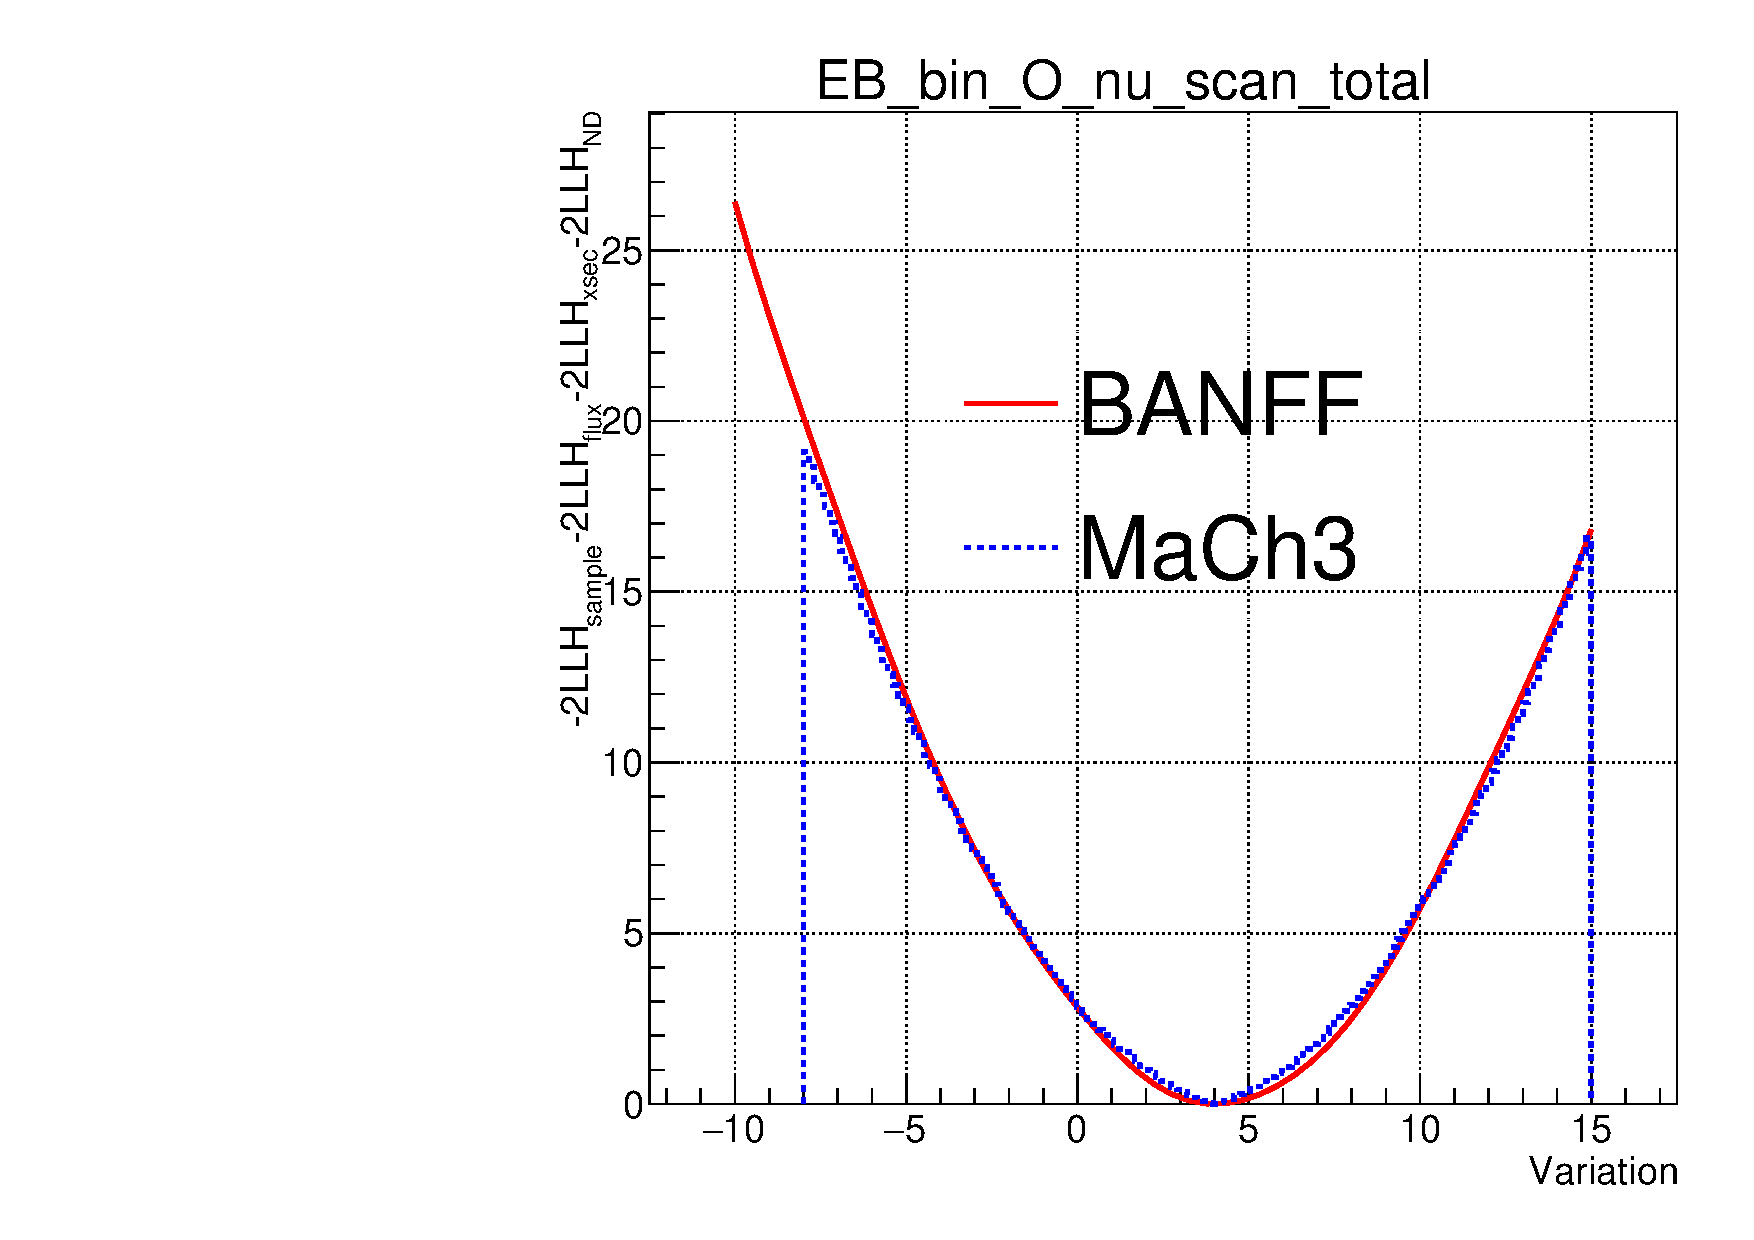
\includegraphics[width=0.73\linewidth]{figs/EB_dial_O_nu_full_FullLLH}
  \caption{$E_{b}\nu$ O}
\end{subfigure}
\begin{subfigure}{.48\textwidth}
  \centering
  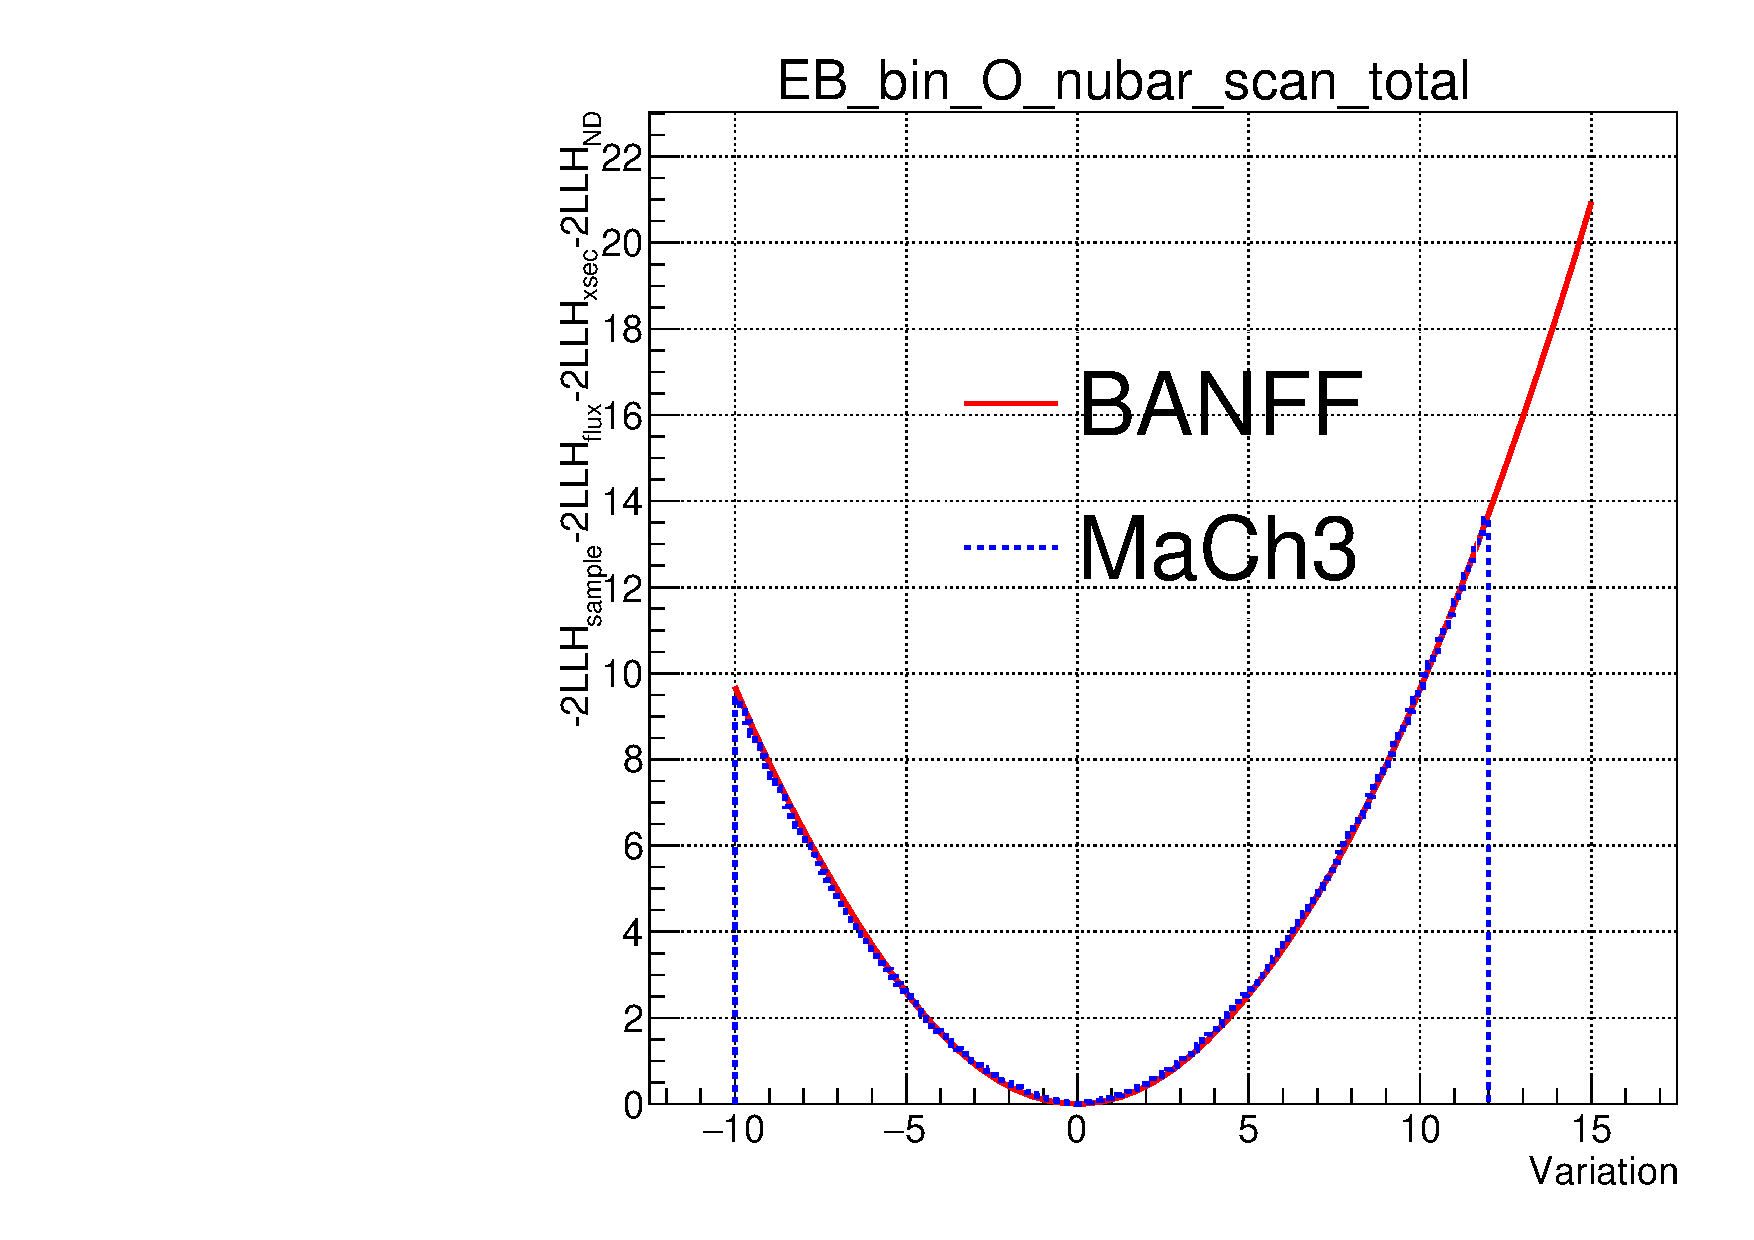
\includegraphics[width=0.73\linewidth]{figs/EB_dial_O_nubar_full_FullLLH}
  \caption{$E_{b}\bar{\nu}$ O}
\end{subfigure}
\caption{Comparison of log-likelihood scans for the two near detector analysis. The good, but not perfect, agreement shows that the effective bin-by-bin reweighting the BANFF use will closely, but not perfectly, replicate the effect of the event-by-event direct shifts used in MaCh3.}
\label{fig:EbLLHBANFF}
\end{figure}

The treatment of the binding energy is one of the main differences between the two near detector fitters, and one of the main advantages of this analysis over the BANFF. 

In previous analyses, the binding energy systematic was applied as a shape parameter. The change in removal energy was propagated to a change in the $p_{\mu}-$cos$\theta_{\mu}$ distributions by reweighting events. However, this method broke down at extreme values of the kinematic variables as changes in the removal energy could change the allowed phase space in unphysical ways. With this implementation, the removal energy was one of the dominant uncertainties in the T2K oscillation analysis. With the direct lepton momentum shift, the removal energy is now a sub-dominant systematic uncertainty, as shown in Section \ref{sec:jointeb}. The treatment of the binding energy is therefore also one of the main improvements made of this analysis compared to previous T2K near detector fits.

This is the first time a systematic of this type has been implemented in a T2K analysis. Now that the framework is in place to accommodate such parameters, more systematics could directly shift event kinematics in the future, as discussed in more detail in Section \ref{sec:detbin}. This work could therefore pave the way for improvements to subsequent analyses.

In summary, the new treatment of the binding energy gives a more accurate implementation of the systematic, significantly reduces the uncertainty, and shows that fitting direct shifts to events is a viable method of applying new parameters in the future.

\subsection{Flux}\label{sec:flux}

The flux systematics are determined using the simulation described in Section \ref{sec:fluxsim}. New data is used to regularly update and improve the modelling. This comes from external experiments such as NA61/SHINE\cite{na61}, the T2K beam monitors, and the on-axis near detector INGRID. This analysis is the first to use flux systematics developed from simulation tuned to data from a full T2K target replica, and not just a thinner replica version.

There are six sources of flux uncertainty:

\begin{itemize}

\item Alignment of the proton beam with the target.

\item Number of protons on target.

\item Interactions of protons and produced hadrons with the target.

\item Alignment of the target with the focusing horns.

\item The horn current and produced magnetic field.

\item Modelling of materials in the target and decay volume.

\end{itemize}

The fractional sizes of the different sources of ND280 flux systematic are shown in Figure \ref{fig:fluxsourceND}, for different neutrino signs. The hadron production contribution dominates, and the total uncertainty is $\sim$10$\%$ around the beam peak energy at 600 MeV. The proton beam alignment becomes more significant around 1 GeV. The black dotted line shows the total flux uncertainty using the previous version of the model. This also used the full replica target tuning; the improvement comes from using the latest FLUKA\cite{fluka} release. Similar results are seen for the SK flux uncertainties, shown in Figure \ref{fig:fluxsourceSK}.

\begin{figure}[!htbp]
\begin{subfigure}{.49\textwidth}
  \centering
  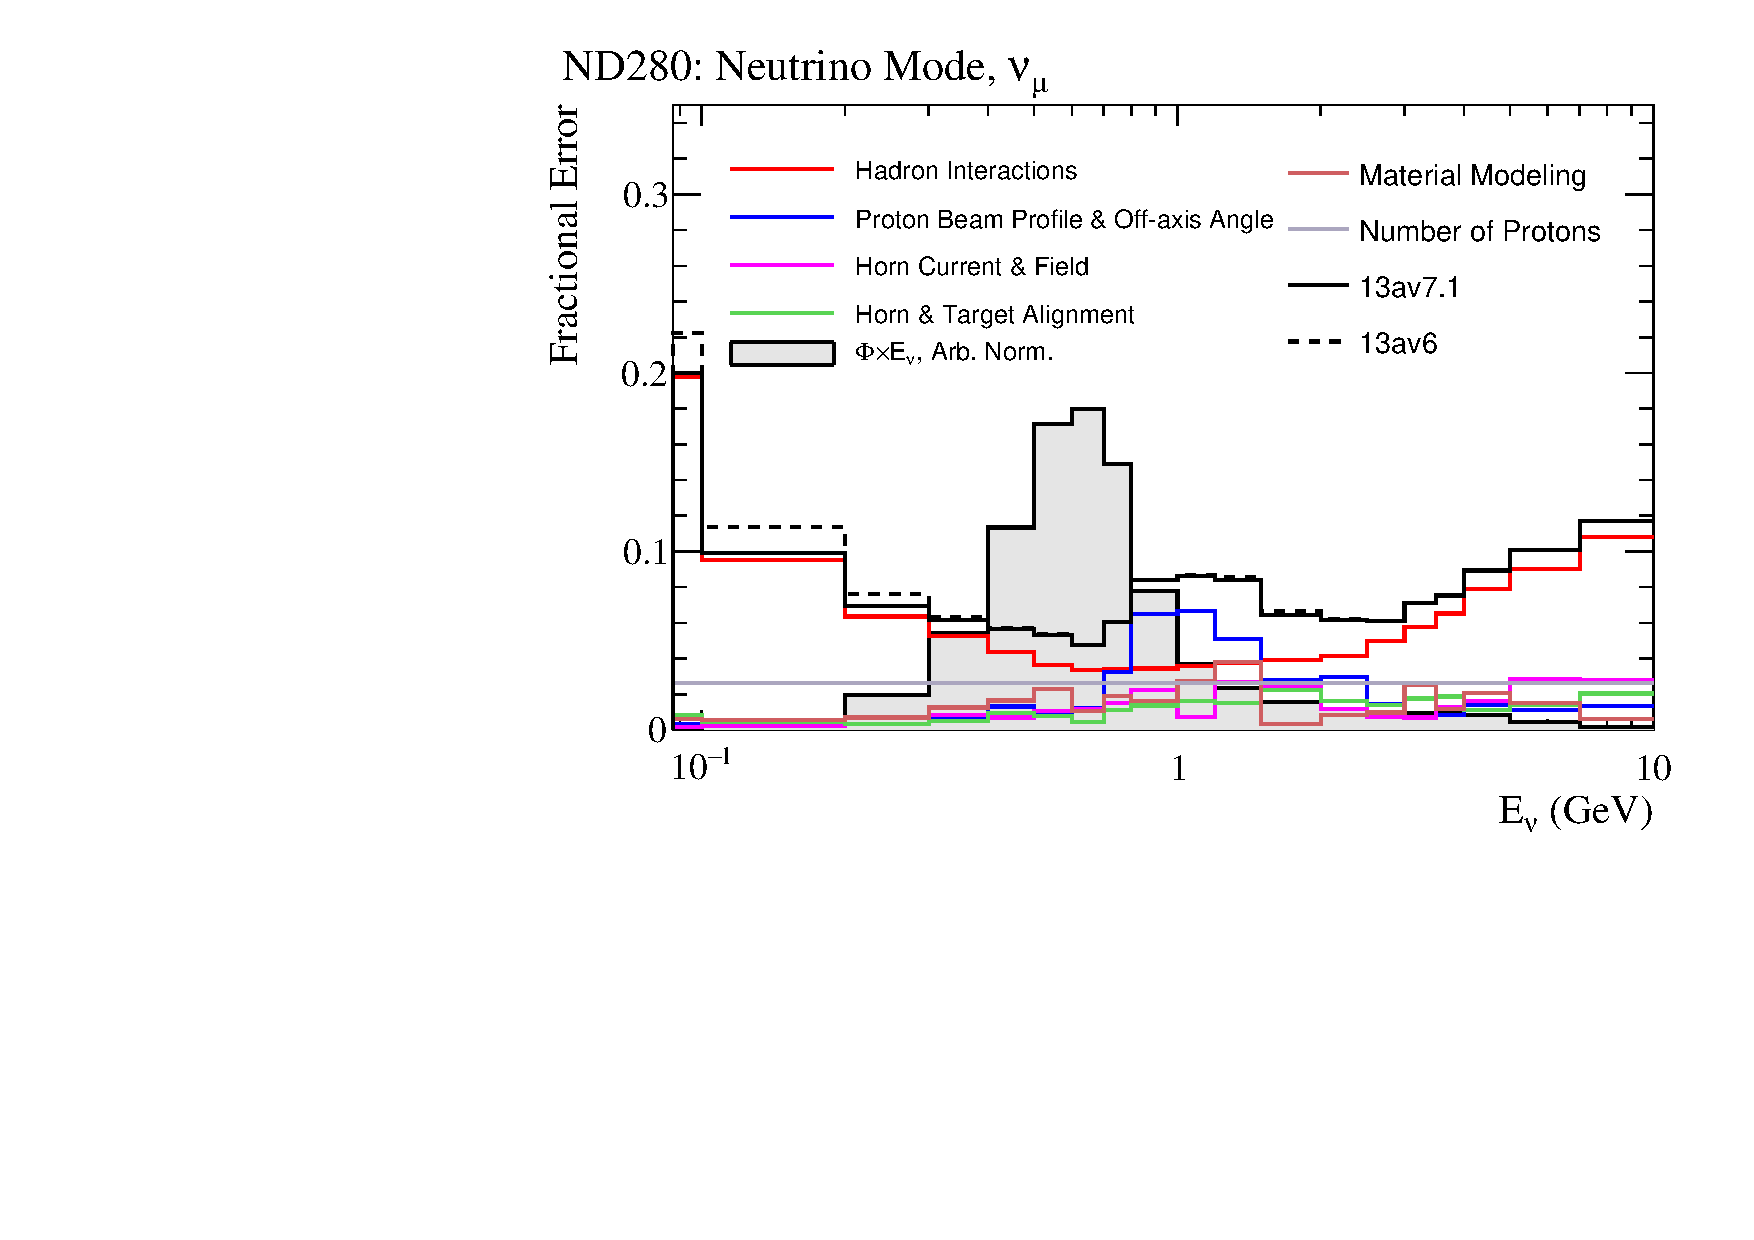
\includegraphics[width=0.99\linewidth]{figs/flux_error_t2k_nd5_fhc_numu}
\end{subfigure}
\begin{subfigure}{.49\textwidth}
  \centering
  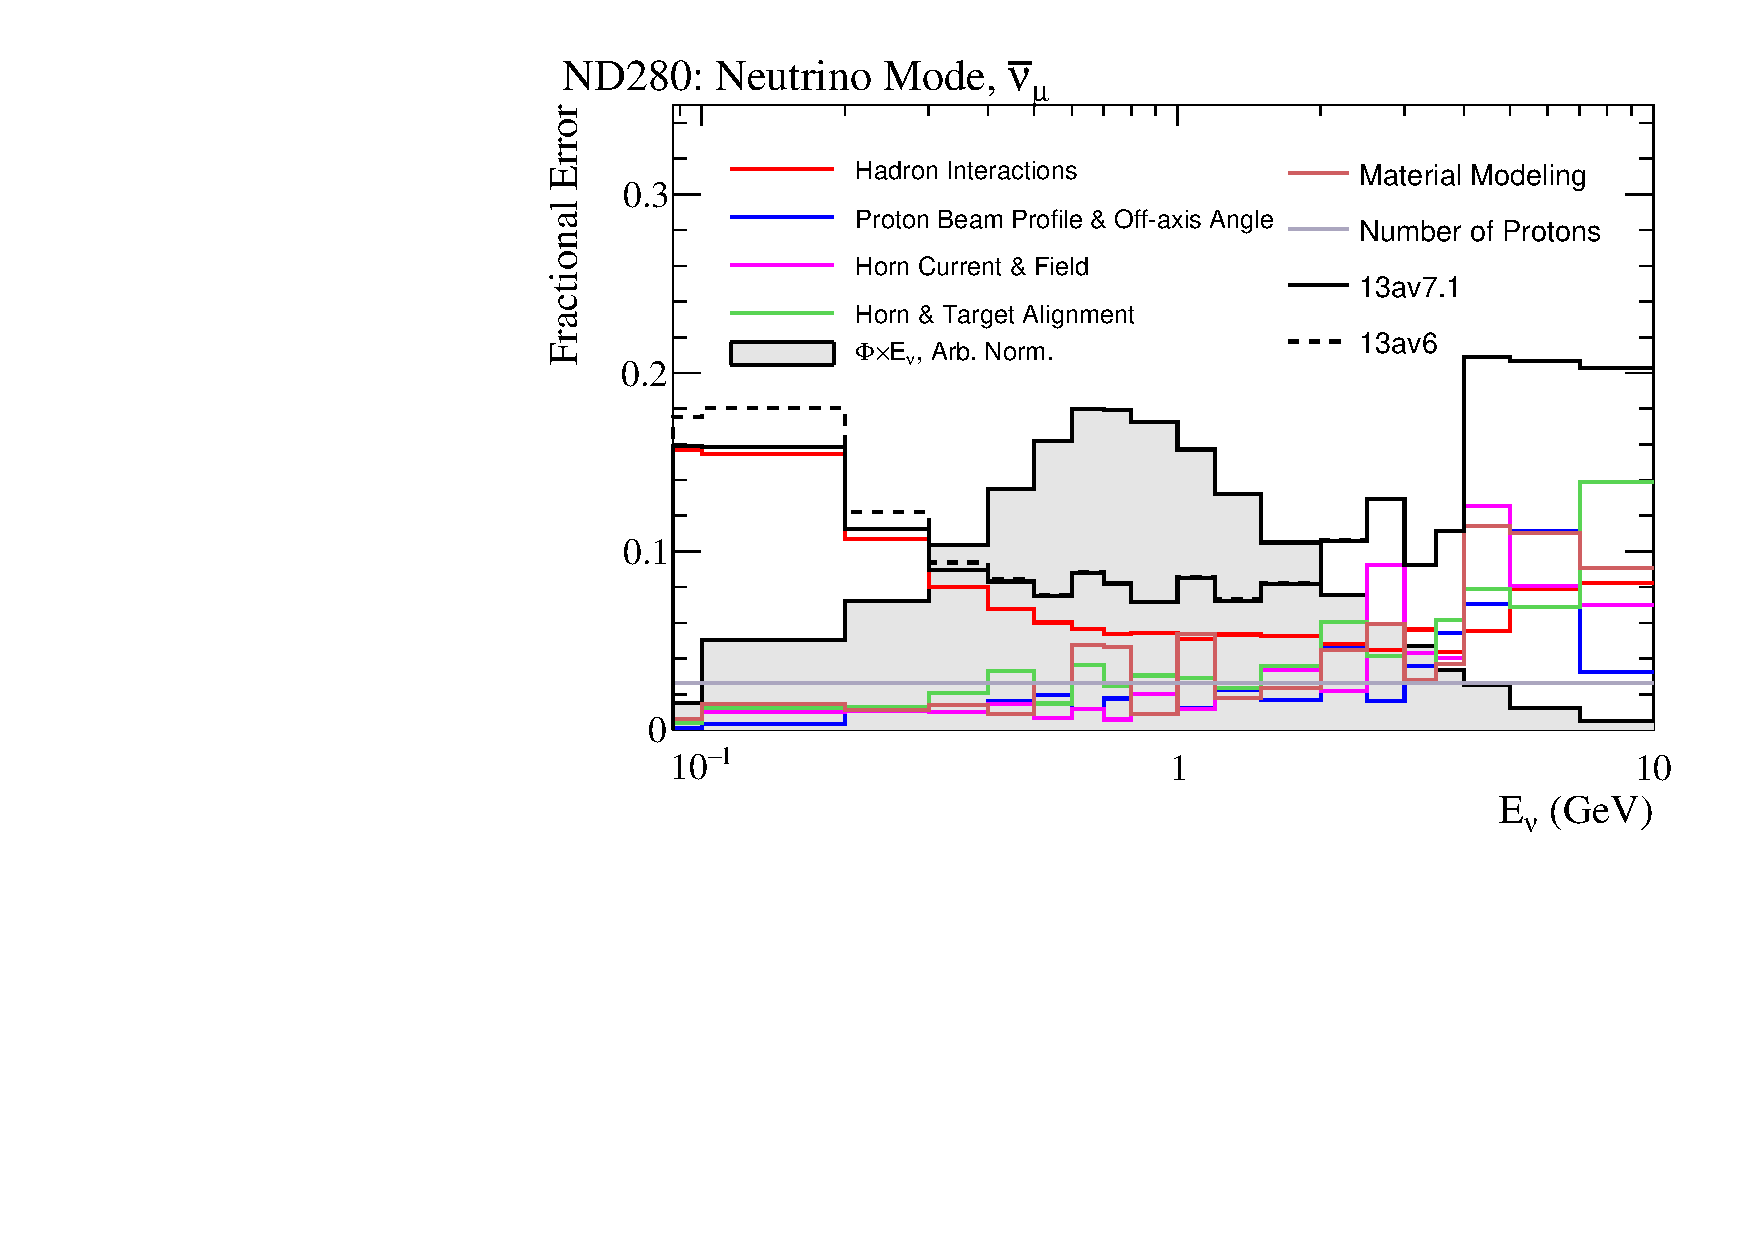
\includegraphics[width=0.99\linewidth]{figs/flux_error_t2k_nd5_fhc_numubar}
\end{subfigure}
\begin{subfigure}{.49\textwidth}
  \centering
  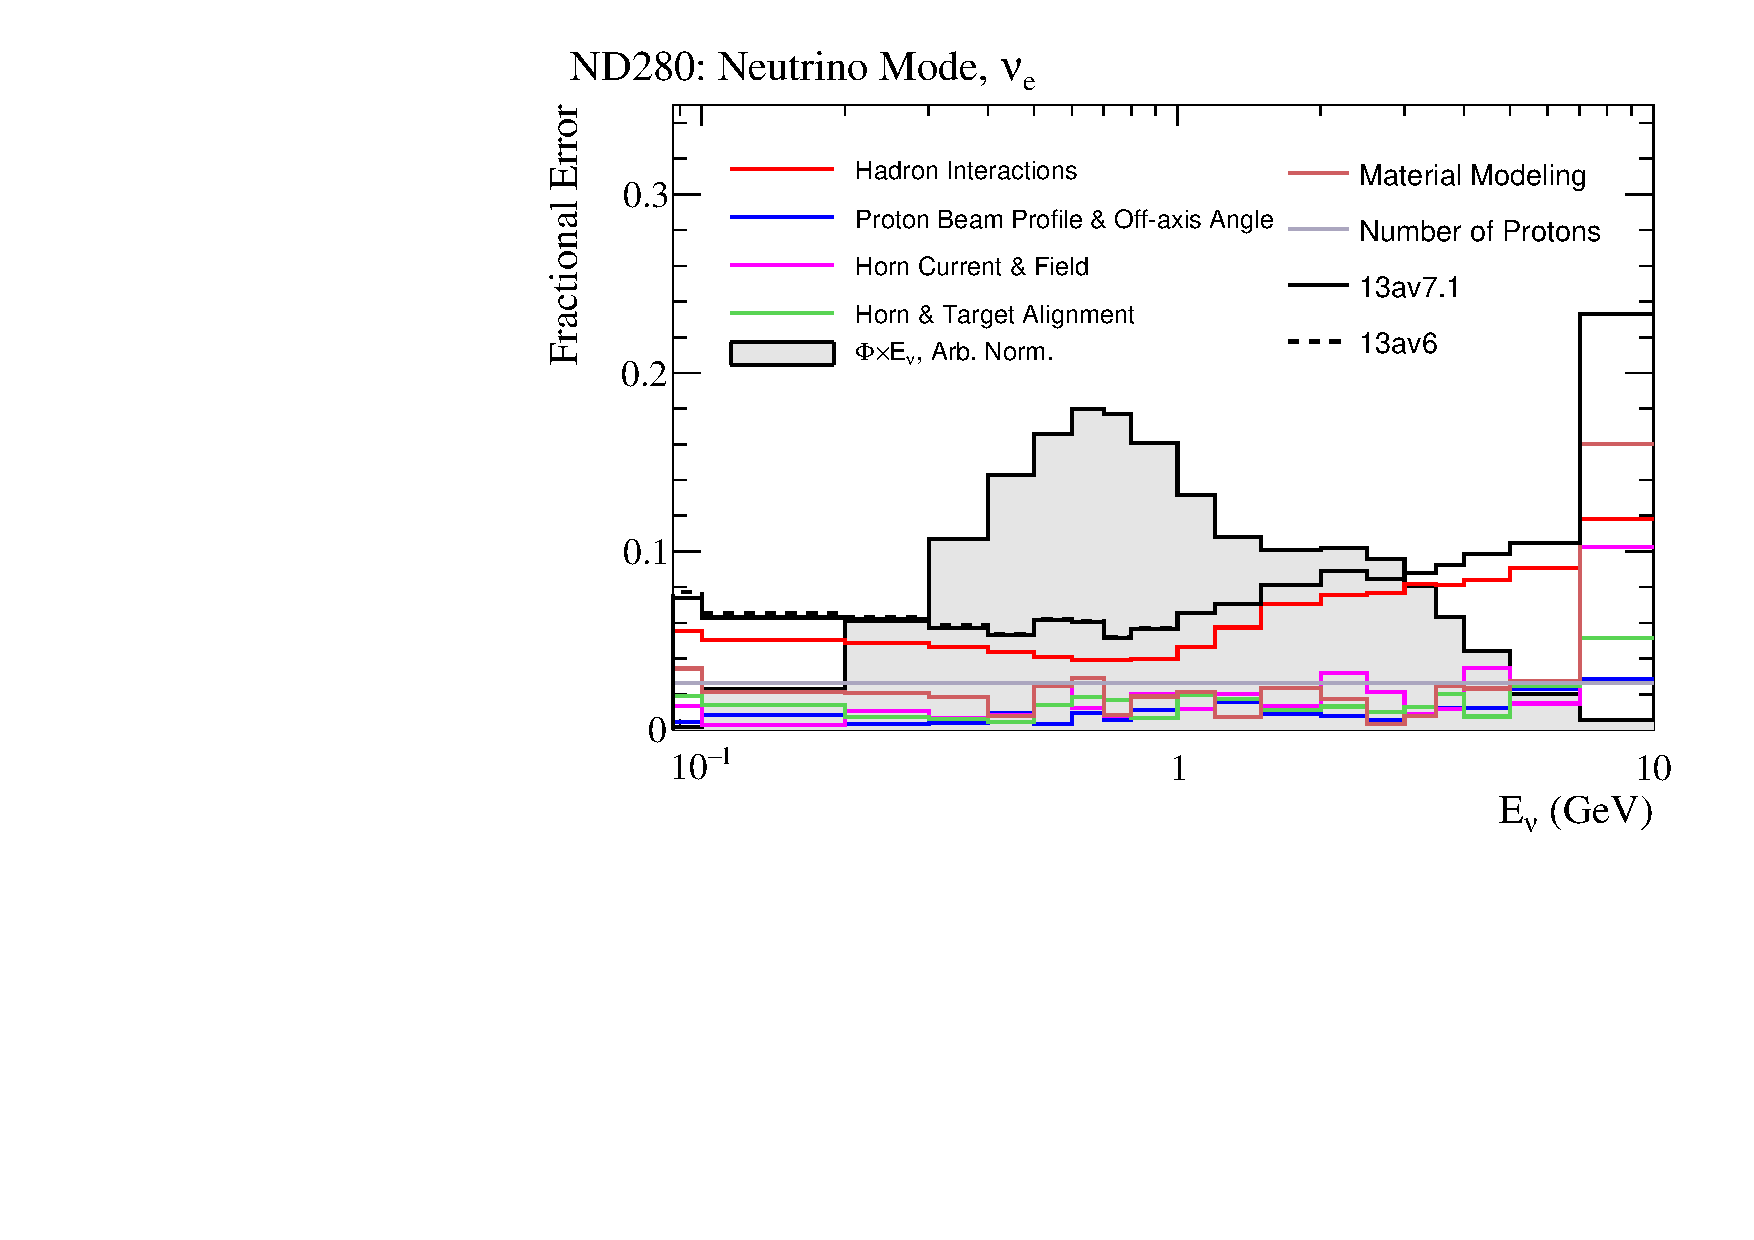
\includegraphics[width=0.99\linewidth]{figs/flux_error_t2k_nd5_fhc_nue}
\end{subfigure}
\begin{subfigure}{.49\textwidth}
  \centering
  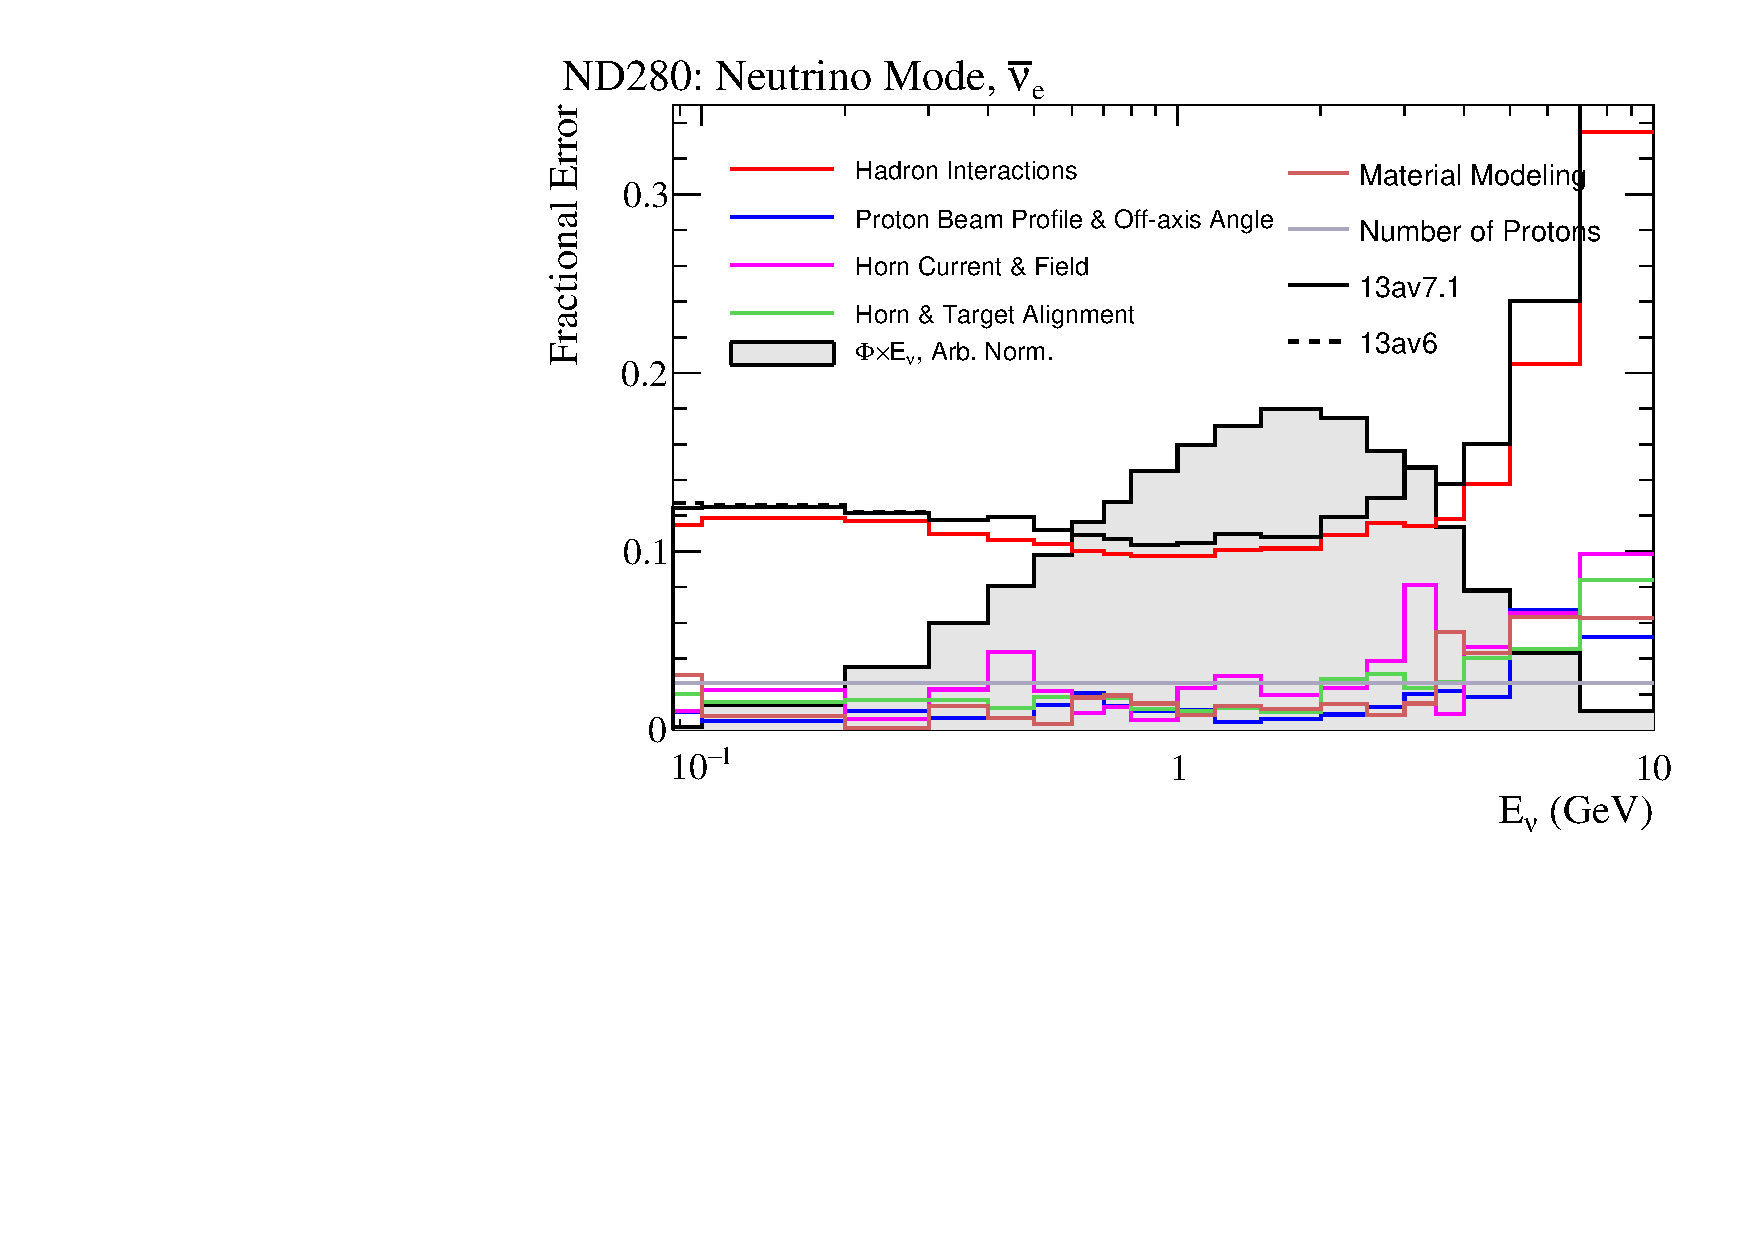
\includegraphics[width=0.99\linewidth]{figs/flux_error_t2k_nd5_fhc_nuebar}
\end{subfigure}
\begin{subfigure}{.49\textwidth}
  \centering
  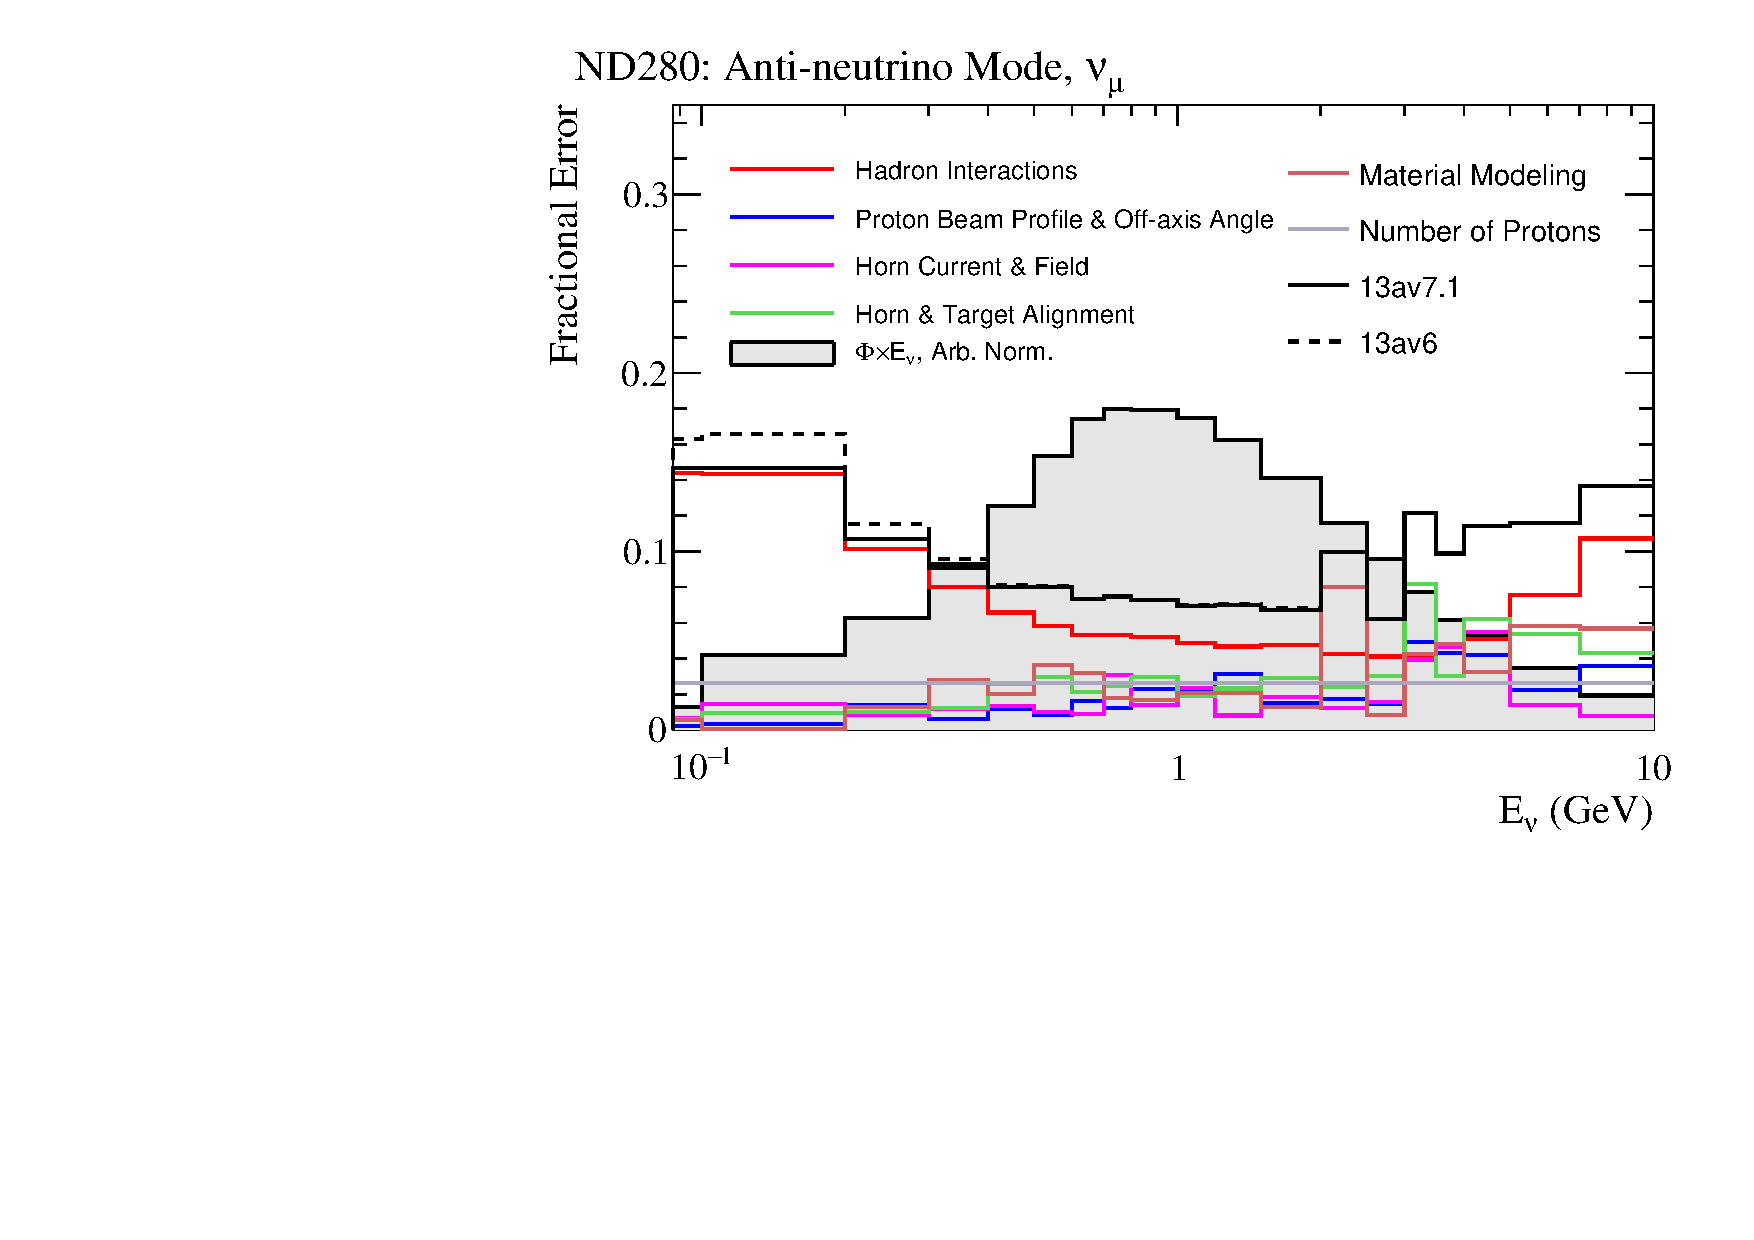
\includegraphics[width=0.99\linewidth]{figs/flux_error_t2k_nd5_rhc_numu}
\end{subfigure}
\begin{subfigure}{.49\textwidth}
  \centering
  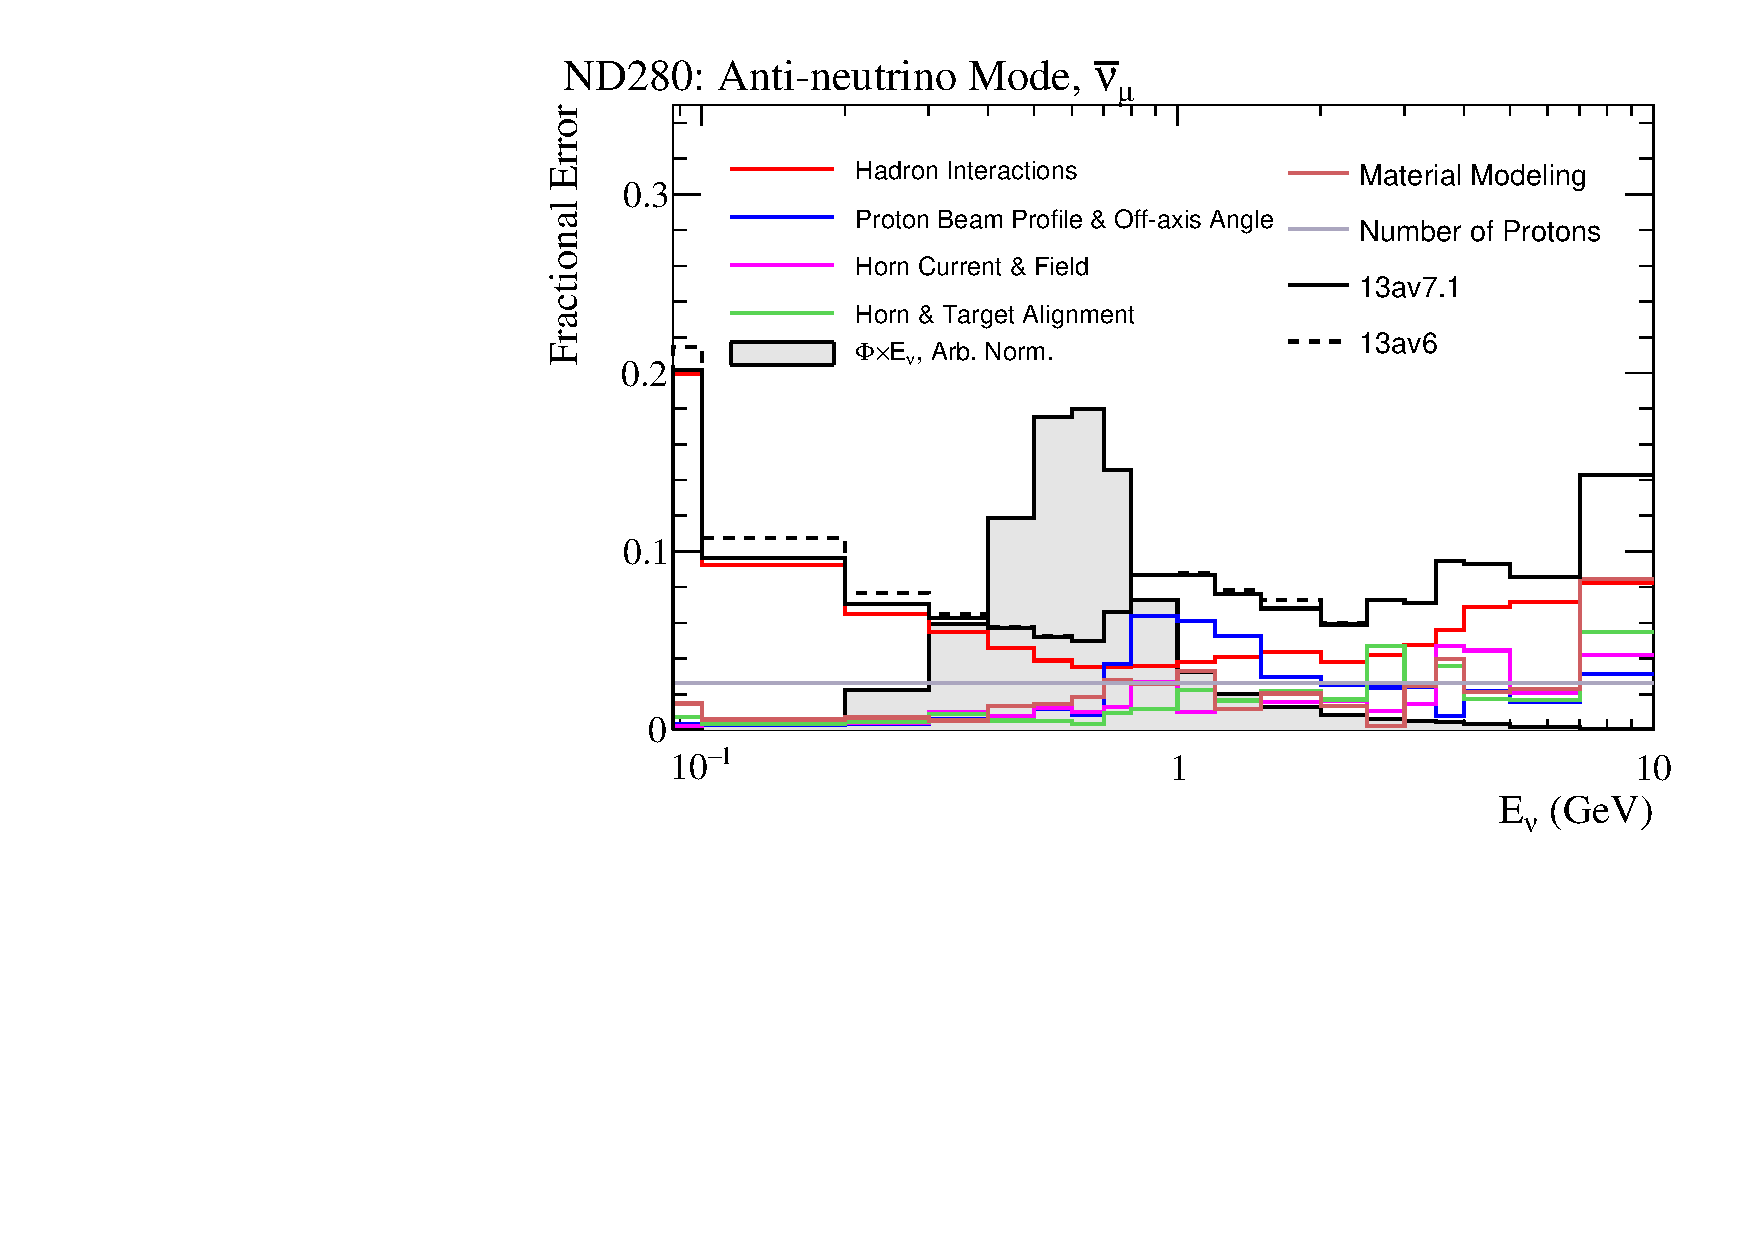
\includegraphics[width=0.99\linewidth]{figs/flux_error_t2k_nd5_rhc_numubar}
\end{subfigure}
\begin{subfigure}{.49\textwidth}
  \centering
  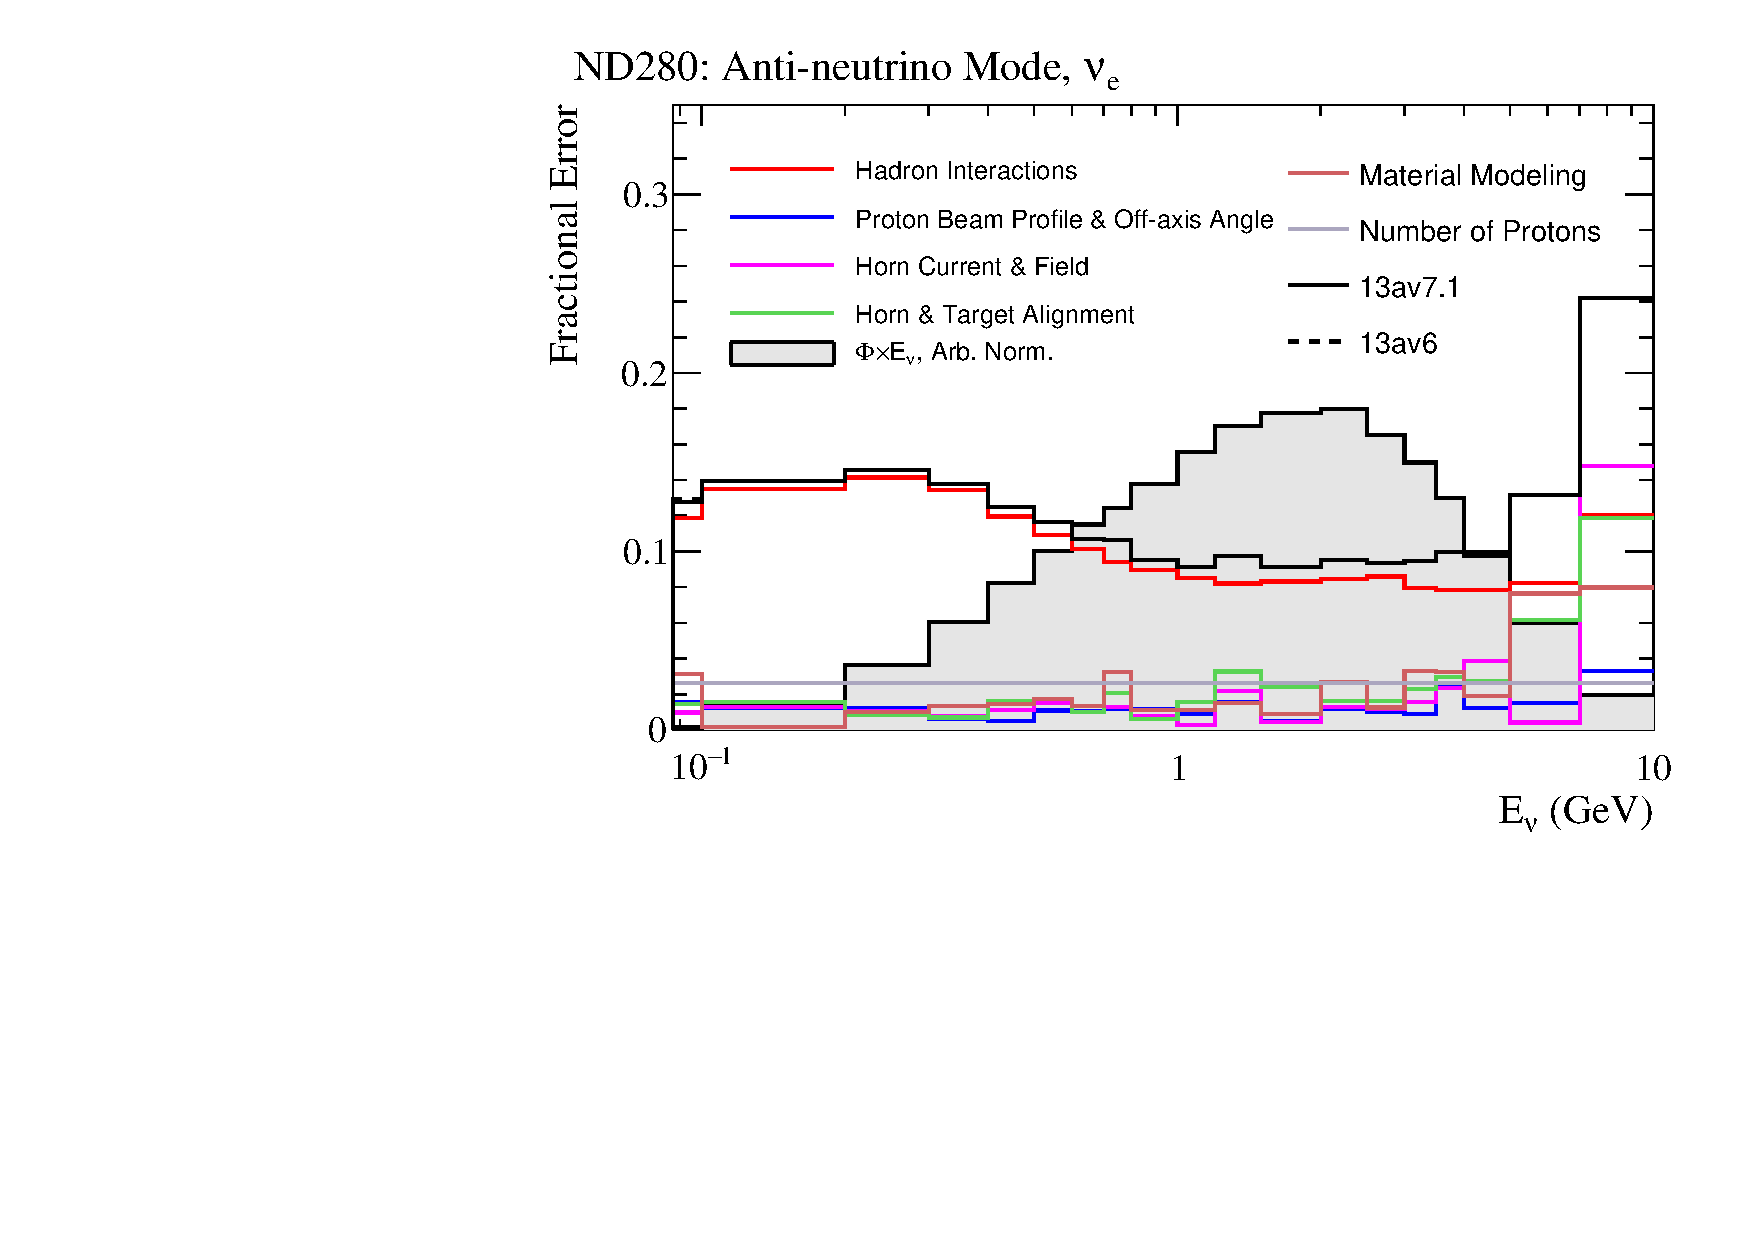
\includegraphics[width=0.99\linewidth]{figs/flux_error_t2k_nd5_rhc_nue}
\end{subfigure}
\begin{subfigure}{.49\textwidth}
  \centering
  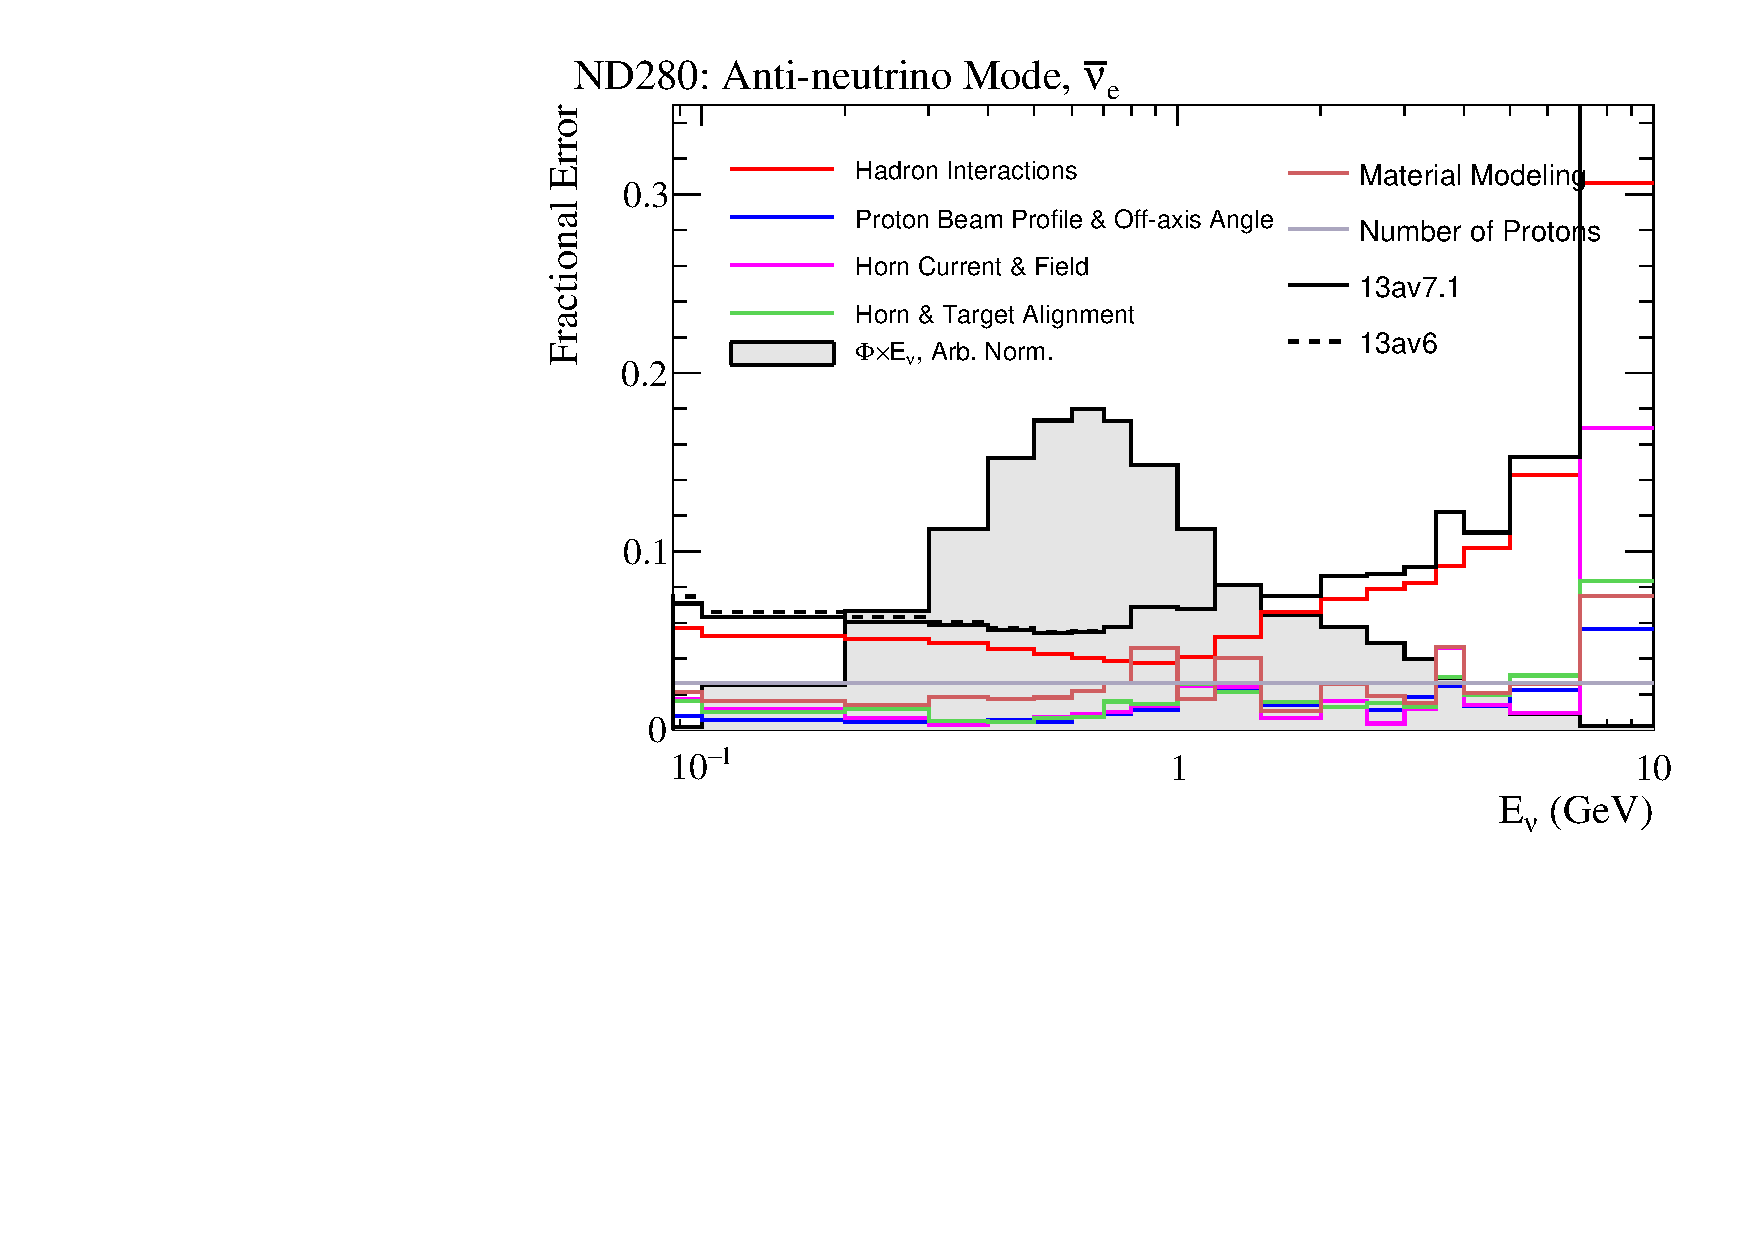
\includegraphics[width=0.99\linewidth]{figs/flux_error_t2k_nd5_rhc_nuebar}
\end{subfigure}
\caption{Relative sizes of the sources of uncertainties in the ND280 flux parameters. ``13av7.1" (black solid line) is the version used in this analysis, and is compared with the previous version, ``13v6" (dotted line).}\label{fig:fluxsourceND}
\end{figure}

\begin{figure}[!htbp]
\begin{subfigure}{.49\textwidth}
  \centering
  \includegraphics[width=0.99\linewidth]{figs/flux_error_t2k_sk_fhc_numu}
\end{subfigure}
\begin{subfigure}{.49\textwidth}
  \centering
  \includegraphics[width=0.99\linewidth]{figs/flux_error_t2k_sk_fhc_numubar}
\end{subfigure}
\begin{subfigure}{.49\textwidth}
  \centering
  \includegraphics[width=0.99\linewidth]{figs/flux_error_t2k_sk_fhc_nue}
\end{subfigure}
\begin{subfigure}{.49\textwidth}
  \centering
  \includegraphics[width=0.99\linewidth]{figs/flux_error_t2k_sk_fhc_nuebar}
\end{subfigure}
\begin{subfigure}{.49\textwidth}
  \centering
  \includegraphics[width=0.99\linewidth]{figs/flux_error_t2k_sk_rhc_numu}
\end{subfigure}
\begin{subfigure}{.49\textwidth}
  \centering
  \includegraphics[width=0.99\linewidth]{figs/flux_error_t2k_sk_rhc_numubar}
\end{subfigure}
\begin{subfigure}{.49\textwidth}
  \centering
  \includegraphics[width=0.99\linewidth]{figs/flux_error_t2k_sk_rhc_nue}
\end{subfigure}
\begin{subfigure}{.49\textwidth}
  \centering
  \includegraphics[width=0.99\linewidth]{figs/flux_error_t2k_sk_rhc_nuebar}
\end{subfigure}
\caption{Relative sizes of the sources of uncertainties in the SK flux parameters. ``13av7.1" (black solid line) is the version used in this analysis, and is compared with the previous version, ``13v6" (dotted line). }\label{fig:fluxsourceSK}
\end{figure}

The flux uncertainty model is parametrised as 100 true neutrino energy bin normalisations, split by neutrino species, horn current mode, and detector. The binnings are as follows:

\begin{itemize}

\item \textbf{ND280 + SK, FHC $\nu_\mu$ + RHC $\bar{\nu_\mu}$:}\\
$E^{true}_{\nu}$: 0, 0.4, 0.5, 0.6, 0.7, 1, 1.5, 2.5, 3.5, 5, 7, 30

\item \textbf{ND280 + SK, FHC $\bar{\nu_\mu}$ + RHC $\nu_\mu$:}\\
$E^{true}_{\nu}$: 0, 0.7, 1, 1.5, 2.5, 30

\item \textbf{ND280 + SK, FHC $\nu_e$ + RHC $\bar{\nu_e}$:}\\
$E^{true}_{\nu}$: 0, 0.5, 0.7, 0.8, 1.5, 2.5, 4, 30

\item \textbf{ND280 + SK, FHC $\bar{\nu_e}$ + RHC $\nu_e$:}\\
$E^{true}_{\nu}$: 0, 2.5, 30

\end{itemize}

In total there are 100 flux parameters, 50 for ND280 and 50 for SK. The SK flux systematics are used in the near detector fit because of their high correlations with their ND280 counterparts. All flux systematics have a prior central value of 1.0, and Gaussian prior uncertainty with width equal to the standard deviation in the fractional covariance matrix, shown in Figure \ref{fig:fluxcov1sample} for the ND280 FHC $\nu_\mu$ parameters. There are larger prefit correlations for parameters with similar energies, particularly at higher energies. The full flux covariance matrix for all samples is shown in Appendix \ref{app:matrices}.

\begin{figure}[!htbp]
\centering
\includegraphics*[width=0.8\textwidth,clip]{figs/fluxcov1sample}
\caption{The flux covariance matrix.}\label{fig:fluxcov1sample}
\end{figure}

\subsection{Detector}\label{sec:det}

The ND280 detector systematicss are modelled using bin normalisation parameters. The underlying systematics are initially varied to see the change to the number of events in each $p_{\mu} - cos \theta_{\mu}$ bin. These systematics are divided into 17 groups:

\begin{itemize}

\item \textbf{TPC Field Distortions:} The magnetic field applied in ND280 is not perfectly uniform, and so there are field distortions in the TPCs. These are measured by calibration lasers with the magnet both on and off.

\item \textbf{TPC Momentum Scale:} The uncertainty in the magnetic field causes an uncertainty in the measured momentum within the TPC. Four hall probes within ND280 provide scaling factors applied to the field strength on the MC.

\item \textbf{TPC Momentum Resolution:} There is a discrepancy between the MC and data momentum resolutions in the TPCs, which is not well understood. To account for this, MC TPC tracks are smeared so that the resolution matches that of data. 

\item \textbf{TPC PID:} The pulls between the measured and predicted energy loss is used to identify particles in the TPC, as discussed in Section \ref{sec:tpc}. The difference between the mean MC and data pulls is applied as a systematic uncertainty on the TPC PID.

\item \textbf{TPC Cluster Efficiency:} There are differences between the reconstruction of clusters of hits in the data and MC. An uncertainty is applied, correlated between horizontal and vertical clusters to account for this. It is calculated using control samples of both beam and cosmic trigger events.

\item \textbf{TPC Tracking Efficiency:} The efficiency of the TPC reconstruction algorithm successfully merging hits into tracks is measured for control samples of both beam and cosmic trigger events. The difference between the efficiencies obtained for data and MC is applied as a systematic.

\item \textbf{TPC Charge ID Efficiency:} There are two sources of uncertainty in the TPC charge identification: the efficiency of the initial TPC charge being correct, and the probability of the TPC charge sign being reversed in the overall charge identification. The TPC Charge ID uncertainty is applied as the probability of the overall charge being different from the TPC reconstructed charge.

\item \textbf{TPC-FGD Matching Efficiency:} The efficiency of matching FGD and TPC tracks was calculated using a control sample of events with a high angle with respect to the neutrino beam, that passed through at least two TPCs. The difference in the efficiency found for data and MC is applied as a systematic.

\item \textbf{FGD PID:} The pulls between the measured and predicted energy loss is used to identify particles in the FGD, as discussed in Section \ref{sec:fgd}. The difference between the mean MC and data pulls is applied as a systematic uncertainty on the FGD PID.

\item \textbf{FGD Time of Flight:} For tracks passing through FGD1 and FGD2, the hit times in each FGD are used to determine the direction of the track. The uncertainty on the time of flight can therefore affect which FGD the event was reconstructed as having occured in. Analysis, rather than control, samples were used to measure the time of flight for data and MC events. All reconstructed time of flights are smeared with the discrepancy as an uncertainty.

\item \textbf{FGD Hybrid Tracking Efficiency:} The efficiency of reconstructing FGD-only tracks in the presence of FGD-TPC matched tracks is calculated for a set of GEANT-4 generated stopping protons and pions in a control sample of events with either one reconstructed track entering the TPC, or two tracks which both enter the TPC. The difference between the efficiencies for data and MC is applied as a systematic uncertainty.

\item \textbf{Michel Electron Efficiency:} The efficiency of detecting Michel electrons depends on the probability of the electron producing enough hits in the FGD to pass the selection cut, and the purity of the cut itself. The efficiency was measured for a control sample of cosmic trigger events, and was defined as the probability to detect a Michel electron that was expected from the presence of a stopped muon in the FGD.

\item \textbf{Out of Fiducial Volume (OOFV) Background:} Events outside the fiducial volume can be misreconstructed as being being inside the fiducial volume. These could be events that occurred in the first two layers of FGD1, the first layer of FGD2, or in one of the other sub-detectors. The background rate was calculated for beam trigger events, and the discrepancy between the measurement for data and MC is applied as a systematic uncertainty.

\item \textbf{Sand Muon Background:} Interactions from beam neutrinos can occur in the sand outside the near detector pit but look similar to events in the FGDs, forming a background rate. The rate from a dedicated simulation is compared to data to calculate the associated uncertainty.

\item \textbf{Pile-Up:} Out-of-fiducial volume events being coincident with in-fiducial volume CC-inclusive events in the FGDs can lead to CC-inclusive events being rejected by the external veto cut described in Section \ref{sec:sel}. The difference in number of events per bunch in the data and MC is applied as systematic uncertainty to account for this effect.

\item \textbf{Pion Secondary Interactions (SI):} Pions produced by neutrino interactions at ND280 can interact within the detector. This causes pion detection inefficiencies. An uncertainty is applied to account for this effect, calculated from the difference between pion SI cross-sections measured in data and MC.

\item \textbf{FGD Mass:} The uncertainty on the FGD masses affects the number of target nuclei, and so can change the total event rate. Differences between the measured and simulated FGD masses are applied as a systematic uncertainty.

\end{itemize}

Each of these systematics is applied in one of three different ways:

\begin{itemize}

\item \textbf{Observable Variable Systematic:} These are smearings that are applied to reconstructed variables. The selection algorithm is then rerun, and so smeared events can change their topology, selection, and which track the lepton candidate is.

\item \textbf{Efficiency-Like Systematics:} These are uncertainties on detection and reconstruction efficiencies, which are applied as weights to the event after selection.

\item \textbf{Normalisation Systematics:} These are overall normalisation changes applied directly to events to scale rates up or down.

\end{itemize}

\begin{center}
\begin{table}
\center
\large
\begin{tabular}{ c||c|c}
\hline
\hline
\textbf{Systematic Source} & \textbf{Type} & \textbf{Prior Shape} \\
\hline
\hline
\textbf{B Field Distortions} & Observable & Flat \\ \hline
\textbf{TPC Momentum Scale} & Observable & Gaussian \\ \hline
\textbf{TPC Momentum Resolution} & Observable & Gaussian \\ \hline
\textbf{TPC PID} & Observable & Gaussian \\ \hline
\textbf{TPC Cluster Efficiency} & Efficiency-Like & Gaussian \\ \hline
\textbf{TPC Tracking Efficiency} & Efficiency-Like & Gaussian \\ \hline
\textbf{TPC Charge ID Efficiency} & Efficiency-Like & Gaussian \\ \hline
\textbf{TPC-FGD Matching Efficiency} & Efficiency-Like & Gaussian \\ \hline
\textbf{FGD PID} & Observable & Gaussian \\ \hline
\textbf{FGD ToF} & Observable & Gaussian \\ \hline
\textbf{FGD Hybrid Tracking Efficiency} & Efficiency-Like & Gaussian \\ \hline
\textbf{Michel Electron Efficiency} & Efficiency-Like & Gaussian \\ \hline
\textbf{OOFV Background} & Normalisation & Gaussian \\ \hline
\textbf{Sand Muon Background} & Normalisation & Gaussian \\ \hline
\textbf{Pile-Up} & Normalisation & Gaussian \\ \hline
\textbf{Pion Secondary Interactions} & Normalisation & Gaussian \\ \hline
\textbf{FGD Mass} & Normalisation & Gaussian \\ 
\hline
\hline
\end{tabular}
\caption{ND280 detector systematics, and their propagation type and prior uncertainty shape.}
\label{tab:detsyst}
\end{table}
\end{center}

The type of each of the 17 systematics is shown in Table \ref{tab:detsyst}, along with whether they have a Gaussian or flat prior uncertainty.

In theory, these systematics could be applied on an event by event basis and fitted individually. However, this is not computationally feasible on the timescales required for the oscillation analysis. Instead, each systematic is varied 2000 times and the MC reweighted. This gives a distribution of 2000 number of events for each $p_{\mu}-$cos$\theta_{\mu}$ bin. The mean and width of a Gaussian fitted to each of these distributions becomes the prior central value and uncertainty for a normalisation parameter applying to that bin. However, the number of fit bins is large, and so to reduce the number of fit parameters, adjacent bins with similar responses to the systematic variations are merged, so the detector binning is coarser than the fit binning. Studies of different detector binnings are presented in Section \ref{sec:detbin}.

This process assumes the shape of the underlying systematics are Gaussian. This is the case for the majority of bins, four of which are shown in Figure \ref{fig:detgaussbins}. In previous analyses, the MC statistics uncertainty was included in the ND280 detector covariance instead of as an extra term in the log-likelihood calculation, and so a Gaussian fitted to the distribution of number of events in each bin with and without the MC stats uncertainty are shown.

However, several bins exhibit non-Gaussian behaviour, as shown in Figure \ref{fig:detnongaussbins}.

\begin{figure}[h]
\centering
\begin{subfigure}{.49\textwidth}
  \centering
  \includegraphics[width=0.95\linewidth]{figs/detbin_allsysts5}
\end{subfigure}
\begin{subfigure}{.49\textwidth}
  \centering
  \includegraphics[width=0.95\linewidth]{figs/detbin_allsysts253}
\end{subfigure}
\begin{subfigure}{.49\textwidth}
  \centering
  \includegraphics[width=0.95\linewidth]{figs/detbin_allsysts430}
\end{subfigure}
\begin{subfigure}{.49\textwidth}
  \centering
  \includegraphics[width=0.95\linewidth]{figs/detbin_allsysts535}
\end{subfigure}
\caption{Distribution of number of events in selected Gaussian distributed bins after 2000 throws of all detector systematics. The red and green lines show Gaussians fitted with and without the MC statistical uncertainty included, and the dotted black line shows the nominal number of events.}
\label{fig:detgaussbins}
\end{figure}

\begin{figure}[h]
\centering
\begin{subfigure}{.49\textwidth}
  \centering
  \includegraphics[width=0.95\linewidth]{figs/detbin_allsysts97}
\end{subfigure}
\begin{subfigure}{.49\textwidth}
  \centering
  \includegraphics[width=0.95\linewidth]{figs/detbin_allsysts103}
\end{subfigure}
\begin{subfigure}{.49\textwidth}
  \centering
  \includegraphics[width=0.95\linewidth]{figs/detbin_allsysts258}
\end{subfigure}
\begin{subfigure}{.49\textwidth}
  \centering
  \includegraphics[width=0.95\linewidth]{figs/detbin_allsysts570}
\end{subfigure}
\caption{Distribution of number of events in selected non-Gaussian distributed bins after 2000 throws of all detector systematics. The red and green lines show Gaussians fitted with and without the MC statistical uncertainty included, and the dotted black line shows the nominal number of events.}
\label{fig:detnongaussbins}
\end{figure}

To investigate which of the underlying detector systematics is causing the non-Gaussianity, each was switched off one-by-one and the variations repeated. It was found that when all systematics but the Pion SI are left on, the distributions in the misbehaving bins are more Gaussian. These are shown in Figure \ref{fig:detnopisibins}. This suggests that the pion SI is the only one of the detector systematics with a significantly non-Gaussian distribution. As the effect only manifests in a small number of bins, it is not too concerning for this analysis.

\begin{figure}[h]
\centering
\begin{subfigure}{.49\textwidth}
  \centering
  \includegraphics[width=0.95\linewidth]{figs/detbin_nopisi97}
\end{subfigure}
\begin{subfigure}{.49\textwidth}
  \centering
  \includegraphics[width=0.95\linewidth]{figs/detbin_nopisi103}
\end{subfigure}
\begin{subfigure}{.49\textwidth}
  \centering
  \includegraphics[width=0.95\linewidth]{figs/detbin_nopisi258}
\end{subfigure}
\begin{subfigure}{.49\textwidth}
  \centering
  \includegraphics[width=0.95\linewidth]{figs/detbin_nopisi570}
\end{subfigure}
\caption{Distribution of number of events in selected bins after 2000 throws of all detector systematics but the pion SI. The red and green lines show Gaussians fitted with and without the MC statistical uncertainty included, and the dotted black line shows the nominal number of events.}
\label{fig:detnopisibins}
\end{figure}

\subsubsection{Detector Binning}\label{sec:detbin}

The choice of detector binning is a trade-off of having as close to the fit binning as possible to obtain more accurate results, without introducing too many parameters to feasibly fit. To investigate the effect of merging detector bins, detector covariances with different binnings were produced. The binnings were produced by requiring different criteria to merge adjacent bins. These criteria were based on the number of events in a bin before applying the detector systematics, the change in the number of events by applying the systematics, and the difference between the covariance of bins. These correspond to merging bins with few events, bins where the effect of the systematics are small, and bins with similar response to the systematics respectively. The exact criteria for merging bins used were:

\begin{itemize}

\item $<$ 1 event in a bin, or $<$ 1 event change from applying the systematics, or $< 10\%$ difference in covariance between bins. This produced 179 merged bins.

\item $<$ 1 event in a bin, or $<$ 1 event change from applying the systematics, or $< 5\%$ difference in covariance between bins. This produced 574 merged bins.

\item $<$ 1 event in a bin, or $<$ 0.5 event change from applying the systematics, or $< 5\%$ difference in covariance between bins. This produced 1347 merged bins.

\end{itemize}

A covariance using the fit binning as the detector binning was also produced. As in these studies the fit binning used was the uniform-rectangular set defined in Appendix \ref{app:bintemplates}, this corresponded to 4238 bins.

Fits were run using each of these four detector covariances, using an intermediate cross-section model including parts of the 2017 analysis parametrisation described in \cite{tn315}, and parts of the 2020 analysis parametrisation described in Section \ref{sec:xsec}. To avoid tuning the detector binning on data, fake data was produced by setting the cross-section parameters to their best fit values from the 2017 analysis and reweighting the runs 2-6 nominal MC. The MC was then fitted to this fake data.

The result of the fits are shown in Figures \ref{fig:detcovbinfluxND} and \ref{fig:detcovbinfluxSK} for the flux parameters, and Figure \ref{fig:detcovbinxsec} for the cross-section parameters. Although there are several differences between the postfit parameter values, there is no consistent trend of having more bins being closer to the fit binning result, and they are all consistent within uncertainties. Although the 179 fit bin fit is often the most different from the 4238 (fit binning) detector bin fit.

\begin{figure}[!htbp]
\centering
\begin{subfigure}{0.3\textwidth}
  \centering
  \includegraphics[width=0.8\linewidth, trim={5mm  65mm 0mm 0mm}, clip]{figs/detcovbin_leg}
\end{subfigure}
\begin{subfigure}{0.3\textwidth}
  \centering
  \includegraphics[width=0.8\linewidth, trim={5mm  0mm 0mm 105mm}, clip]{figs/detcovbin_leg}
\end{subfigure}
\begin{subfigure}{0.45\textwidth}
  \centering
  \includegraphics[width=0.75\linewidth]{figs/detcovbinflux_0}
  \caption{ND FHC $\nu_{\mu}$}
\end{subfigure}
\begin{subfigure}{0.45\textwidth}
  \centering
  \includegraphics[width=0.75\linewidth]{figs/detcovbinflux_1}
  \caption{ND FHC $\bar{\nu_{\mu}}$}
\end{subfigure}
\begin{subfigure}{0.45\textwidth}
  \centering
  \includegraphics[width=0.75\linewidth]{figs/detcovbinflux_2}
  \caption{ND FHC $\nu_e$}
\end{subfigure}
\begin{subfigure}{0.45\textwidth}
  \centering
  \includegraphics[width=0.75\linewidth]{figs/detcovbinflux_3}
  \caption{ND FHC $\bar{\nu_{e}}$}
\end{subfigure}
\begin{subfigure}{0.45\textwidth}
  \centering
  \includegraphics[width=0.75\linewidth]{figs/detcovbinflux_4}
  \caption{ND RHC $\nu_{\mu}$}
\end{subfigure}
\begin{subfigure}{0.45\textwidth}
  \centering
  \includegraphics[width=0.75\linewidth]{figs/detcovbinflux_5}
  \caption{ND RHC $\bar{\nu_{\mu}}$}
\end{subfigure}
\begin{subfigure}{0.45\textwidth}
  \centering
  \includegraphics[width=0.75\linewidth]{figs/detcovbinflux_6}
  \caption{ND RHC $\nu_e$}
\end{subfigure}
\begin{subfigure}{0.45\textwidth}
  \centering
  \includegraphics[width=0.75\linewidth]{figs/detcovbinflux_7}
  \caption{ND RHC $\bar{\nu_e}$}
\end{subfigure}
\caption{ND280 flux parameters for fake data fits using different detector binnings.}
\label{fig:detcovbinfluxND}
\end{figure}

\begin{figure}[!htbp]
\centering
\begin{subfigure}{0.3\textwidth}
  \centering
  \includegraphics[width=0.8\linewidth, trim={5mm  65mm 0mm 0mm}, clip]{figs/detcovbin_leg}
\end{subfigure}
\begin{subfigure}{0.3\textwidth}
  \centering
  \includegraphics[width=0.8\linewidth, trim={5mm  0mm 0mm 105mm}, clip]{figs/detcovbin_leg}
\end{subfigure}
\begin{subfigure}{0.45\textwidth}
  \centering
  \includegraphics[width=0.75\linewidth]{figs/detcovbinflux_8}
  \caption{SK FHC $\nu_{\mu}$}
\end{subfigure}
\begin{subfigure}{0.45\textwidth}
  \centering
  \includegraphics[width=0.75\linewidth]{figs/detcovbinflux_9}
  \caption{SK FHC $\bar{\nu_{\mu}}$}
\end{subfigure}
\begin{subfigure}{0.45\textwidth}
  \centering
  \includegraphics[width=0.75\linewidth]{figs/detcovbinflux_10}
  \caption{SK FHC $\nu_e$}
\end{subfigure}
\begin{subfigure}{0.45\textwidth}
  \centering
  \includegraphics[width=0.75\linewidth]{figs/detcovbinflux_11}
  \caption{SK FHC $\bar{\nu_{e}}$}
\end{subfigure}
\begin{subfigure}{0.45\textwidth}
  \centering
  \includegraphics[width=0.75\linewidth]{figs/detcovbinflux_12}
  \caption{SK RHC $\nu_{\mu}$}
\end{subfigure}
\begin{subfigure}{0.45\textwidth}
  \centering
  \includegraphics[width=0.75\linewidth]{figs/detcovbinflux_13}
  \caption{SK RHC $\bar{\nu_{\mu}}$}
\end{subfigure}
\begin{subfigure}{0.45\textwidth}
  \centering
  \includegraphics[width=0.75\linewidth]{figs/detcovbinflux_14}
  \caption{SK RHC $\nu_e$}
\end{subfigure}
\begin{subfigure}{0.45\textwidth}
  \centering
  \includegraphics[width=0.75\linewidth]{figs/detcovbinflux_15}
  \caption{SK RHC $\bar{\nu_e}$}
\end{subfigure}
\caption{SK flux parameters for fake data fits using different detector binnings.}
\label{fig:detcovbinfluxSK}
\end{figure}

\begin{figure}[!htbp]
\centering
\begin{subfigure}{0.3\textwidth}
  \centering
  \includegraphics[width=0.8\linewidth, trim={5mm  65mm 0mm 0mm}, clip]{figs/detcovbin_leg}
\end{subfigure}
\begin{subfigure}{0.3\textwidth}
  \centering
  \includegraphics[width=0.8\linewidth, trim={5mm  0mm 0mm 105mm}, clip]{figs/detcovbin_leg}
\end{subfigure}
\begin{subfigure}{0.49\textwidth}
  \centering
  \includegraphics[width=0.95\linewidth]{figs/detcovbinxsec_1}
  \caption{CC0$\pi$}
\end{subfigure}
\begin{subfigure}{0.49\textwidth}
  \centering
  \includegraphics[width=0.95\linewidth]{figs/detcovbinxsec_2}
  \caption{CC1$\pi$, $\nu_e$, CC DIS, and CC coh.}
\end{subfigure}
\begin{subfigure}{0.49\textwidth}
  \centering
  \includegraphics[width=0.95\linewidth]{figs/detcovbinxsec_3}
  \caption{NC.}
\end{subfigure}
\begin{subfigure}{0.49\textwidth}
  \centering
  \includegraphics[width=0.95\linewidth]{figs/detcovbinxsec_4}
  \caption{$\pi$ FSI and $E_b$}
\end{subfigure}
\caption{Interaction parameters for fake data fits using different detector binnings.}
\label{fig:detcovbinxsec}
\end{figure}

Furthermore, when the postfit chains are used to produce posterior predictive distributions at the far detector, there is very little difference seen, as shown in Figure \ref{fig:detbinSK}. This suggests that there are several regions of minima in the $\sim$700 dimensional parameter space which correspond to the same result at SK. 

\begin{figure}[!htbp]
\centering
\begin{subfigure}{.49\textwidth}
  \centering
  \includegraphics[width=0.95\linewidth]{figs/detbin_numu}
  \caption{1R$_{\mu}$}
\end{subfigure}
\begin{subfigure}{.49\textwidth}
  \centering
  \includegraphics[width=0.95\linewidth]{figs/detbin_numubar}
  \caption{RHC 1R$_{\mu}$}
\end{subfigure}
\begin{subfigure}{.49\textwidth}
  \centering
  \includegraphics[width=0.95\linewidth]{figs/detbin_nue}
  \caption{1R$_{e}$}
\end{subfigure}
\begin{subfigure}{.49\textwidth}
  \centering
  \includegraphics[width=0.95\linewidth]{figs/detbin_nuebar}
  \caption{RHC 1R$_{e}$}
\end{subfigure}
\begin{subfigure}{.49\textwidth}
  \centering
  \includegraphics[width=0.95\linewidth]{figs/detbin_nue1pi}
  \caption{1R$_{e}$ 1d.e.}
\end{subfigure}
\caption{SK posterior predictive distributions from near detector fits using different binnings for the detector covariance.}
\label{fig:detbinSK}
\end{figure}

As the far detector prediction was robust to the different detector bin mergings, and previous analyses have shown that having $\sim$600 detector parameters does not cause any issues with fit convergence\footnote{For the 2017 analysis, 556 detector bins were used.}, the 574 bin detector covariance was chosen as the optimum bin merging. The binning is as follows:

\begin{itemize}
\setlength\itemsep{1mm}
\item \textbf{FHC $\nu_{\mu}$ CC0$\pi$:}\\
\textbf{\textit{p} (MeV/c):} 0., 300., 1000., 1250., 1500., 2000., 3000., 5000., 30000.\\
\textbf{cos$\theta$:} -1.0, 0.6, 0.8, 0.85, 0.9, 0.92, 0.98, 0.99, 1.0

\item \textbf{FHC $\nu_{\mu}$ CC1$\pi$:}\\
\textbf{\textit{p} (MeV/c):} 0., 300., 400., 700., 800., 1000., 1500., 2000., 5000., 30000.\\
\textbf{cos$\theta$:} -1.0, 0.6, 0.8, 0.9, 0.92, 0.94, 0.96, 0.98, 0.99, 1.0

\item \textbf{FHC $\nu_{\mu}$ CCOther:} \\
\textbf{\textit{p} (MeV/c):} 0., 300., 400., 700., 800., 900., 1250., 2000., 3000., 5000., 30000.\\
\textbf{cos$\theta$:} -1.0, 0.6, 0.8, 0.85, 0.9, 0.92, 0.96, 0.98, 0.99, 1.0

\item \textbf{RHC $\bar{\nu_{\mu}}$ CC0$\pi$:}\\
\textbf{\textit{p} (MeV/c):} 0., 300., 2000., 4000., 30000.\\
\textbf{cos$\theta$:} -1., 0.6, 0.8, 0.9, 0.96, 1.

\item \textbf{RHC $\bar{\nu_{\mu}}$ CC1$\pi$:}\\
\textbf{\textit{p} (MeV/c):} 0., 500., 30000.\\
\textbf{cos$\theta$:} -1, 0.7, 1.

\item \textbf{RHC $\bar{\nu_{\mu}}$ CCOther:}\\
\textbf{\textit{p} (MeV/c):} 0., 600., 800., 30000.\\
\textbf{cos$\theta$:} -1., 0.7, 0.95, 0.97, 1.

\item \textbf{RHC $\nu_{\mu}$ CC0$\pi$:}\\
\textbf{\textit{p} (MeV/c):} 0., 300., 1500., 30000.\\
\textbf{cos$\theta$:} -1., 0.7, 1.

\item \textbf{RHC $\nu_{\mu}$ CC1$\pi$:}\\
\textbf{\textit{p} (MeV/c):} 0., 600., 800., 30000.\\
\textbf{cos$\theta$:} -1, 0.7, 1.

\item \textbf{RHC $\nu_{\mu}$ CCOther:}\\
\textbf{\textit{p} (MeV/c):} 0., 600., 30000.\\
\textbf{cos$\theta$:} -1., 0.7, 1.

\end{itemize}

In this analysis, another detector covariance was also used for separate fits ran in parallel with the 574 detector bin fits. These fits used the full non-uniform fit binning as the detector binning. As the MC statistics uncertainty was taken out of the detector covariance for this analysis, reducing the terms in the diagonal of the covariance, the number of fit parameters can be reduced using principal component analysis. This could then allow the full fit binning detector covariance to be used in joint near and far detector fits, which was not previously possible as it would introduce too many fit parameters. This was not done for this analysis, but the full fit detector covariances are used in parallel near detector fits (which can accommodate more fit parameters) to study the potential impact.

The 574 binned detector covariance is shown for the FGD1 CC 0$\pi$ sample in Figure \ref{fig:detcorr5741sample}. For each momentum range, the bins correspond to the angle ranges, in increasing order, defined above for the 574 merged bins. Bins with similar angles are strongly correlated with each other, and this correlation increases with angle, particularly for bins which apply to the same momentum range. There is a slight anti-correlation between the highest angle bins, and some of the lower angle bins. Bins with similar momentum ranges are also more strongly correlated to each other than bins corresponding to higher or lower momentum.

The two full detector covariances used are shown in Appendix \ref{app:matrices}, showing similar patterns for all samples.

\begin{figure}[!htbp]
\centering
\includegraphics*[width=0.9\textwidth,clip]{figs/detcov574_1sample}
\caption{The ND280 detector covariance matrix with 574 merged bins for the FGD1 CC 0$\pi$ sample, produced using runs 2-9 MC. The full matrix for all samples is shown in Appendix \ref{app:matrices}.}\label{fig:detcorr5741sample}
\end{figure}

\section{Prefit Corrections and Scalings}\label{sec:corr}

A number of corrections and reweightings are applied to the MC prediction to account for well understood discrepancies between MC and data. These `one-time' weights are applied before the fit, and are not varied in it. 

\begin{itemize}

\item \textbf{POT: } A scaling is applied to every MC event to account for the fact that more MC POT is produced for each run than data POT. The weight applied to each event depends on the run, and is the ratio of the total data POT with good data quality flag to MC POT in the run.

\item \textbf{Pile Up: } The detector efficiency in data is lower than in MC because of the coincidence between neutrino events and interactions involving sand muons. This needs to be applied as MC neutrino interactions within the magnet are simulated separately from sand muons. The correction applied depends on the run, and which FGD the event occurred in.

\item \textbf{Detector: } Precise control studies are used to inform corrections due to well known hardware and reconstruction deficiencies in the TPC d$E/$d$x$ and PID. These are applied on an event by event basis, and are discussed in more detail in \cite{tn212}.

\item \textbf{Flux: } A correction is made to the nominal neutrino flux for tunings to updated replica target data. The value of the weight applied depends on the run and neutrino energy.

\item \textbf{Coulomb: } When the lepton produced in a CCQE neutrino interaction leaves the nucleus, it is either electrostatically attracted to, or repulsed by, the nucleus, depending on its charge. This increases or decreases the momentum of the lepton. To model this, a shift in momentum is applied to CC events. The value of the shift is tuned to electron scattering data \cite{coulombcorr}, and depends on the target nucleus and sign of the lepton, as shown in Table \ref{tab:coulomb}.

\begin{center}
\begin{table}
\center
\begin{tabular}{ c||c|c}
\hline
\hline
\textbf{Target} & \textbf{$p_{\mu^{+}}$ Shift (MeV)} & \textbf{$p_{\mu^{-}}$ Shift (MeV)} \\
\hline
\hline
\textbf{C} & +2.6 & -3.6\\
\textbf{O} & +3.3 & -4.3\\ 
\hline
\hline
\end{tabular}
\caption{Momentum shifts applied to final state leptons in CC events.}
\label{tab:coulomb}
\end{table}
\end{center}

\end{itemize}

All of these one-time corrections, along with the systematics that vary in the fit (apart from the Coulomb shifts and $E_{b}$ parameters), are applied to the raw MC as multiplicative weights on an event-by-event basis. This produces the nominal MC prediction which is ultimately fitted to the data.

\section{Data}\label{sec:data}

T2K has been taking data in distinct run periods since 2010, in both FHC and RHC beam mode. The beam power has been steadily increasing over this time, as shown in Figure \ref{fig:pot}.

MC is produced for each run period individually, so that run-by-run effects such as the beam and detector configurations, and tunings to in-situ beam measurements, can be accounted for.

Table \ref{tab:pot} shows the amount of MC POT produced in each run, along with the amount of data taken with good data quality flag (defined as POT collected with all sub-detectors of ND280, and the data acquisition system, online). Over runs 2-9, the overall efficiency of good data taking was $\sim$69$\%$.

\begin{center}
\begin{table}
\center
\large
\begin{tabular}{ c|c||c|c}
\hline
\hline
\textbf{Run} & \textbf{Beam Mode} & \textbf{Data POT ($\times10^{19}$)} & \textbf{MC POT ($\times10^{19}$)} \\
\hline
\hline
\textbf{2a} & \textbf{FHC} & 3.59 & 167.99 \\
\textbf{2w} & \textbf{FHC} & 4.34 & 120.38 \\
\hline
\textbf{3} & \textbf{FHC} & 15.81 & 307.77 \\
\hline
\textbf{4a} & \textbf{FHC} & 17.83 & 361.23 \\
\textbf{4w} & \textbf{FHC} & 16.43 & 361.22 \\
\hline
\textbf{5} & \textbf{RHC} & 4.35 & 221.10 \\
\hline
\textbf{6} & \textbf{RHC} & 34.09 & 346.99 \\
\hline
\textbf{7} & \textbf{RHC} & 24.38 & 333.00 \\
\hline
\textbf{8a} & \textbf{FHC} & 41.50 & 361.10 \\
\textbf{8w} & \textbf{FHC} & 15.81 & 254.23 \\
\hline
\textbf{9} & \textbf{RHC} & 20.54 & 245.61 \\
\hline \hline
\textbf{Total} & \textbf{FHC}  & 115.31 & 1933.89 \\ 
& \textbf{RHC} & 83.36 & 1146.69 \\
& \textbf{FHC+RHC}  & 198.67  & 3080.59 \\
\hline
\hline

\end{tabular}
\caption{Collected and generated POT for the run periods used in this analysis.}
\label{tab:pot}
\end{table}
\end{center}
\vspace{-0.8cm}

Significantly more MC is produced than data, with the weights and corrections described in the previous sections bringing the MC prediction comparable to data. 

Runs with an `a' or `w' suffix refer to whether the P0D was filled with air (a) or water (w) during the run. These are separated, despite being part of the same global run, as the MC production requires different geometries to be used for these two different configurations. Runs without a suffix had a consistent P0D filling for the entire run. This was water for runs 5, 7, and 9, and air for runs 3 and 6.

The most recent data taking period, run 10, finished in February 2020, but had not been through the full processing in time for this analysis. Run 1 was not included as not all of the sub-detectors of ND280 were online.

\newpage
